% !BIB program = biber

%%%% Time-stamp: <2018-03-24 14:05:09 vk>
%% ========================================================================
%%%% Disclaimer
%% ========================================================================
%%
%% created by
%%
%%      Karl Voit
%%

%% ========================================================================
%%%% Basic settings
%% ========================================================================
%% (idea of using newcommands for basic documentclass settings from: Thomas Schlager)

\newcommand{\mypapersize}{A4}
%% e.g., "A4", "letter", "legal", "executive", ...
%% The size of the paper of the resulting PDF file.

\newcommand{\mylaterality}{twoside}
%% "oneside" or "twoside"
%% Either you are creating a document which is printed on both, left pages
%% and right pages (twoside) or you create a document which is printed
%% on right pages only (oneside).

\newcommand{\mydraft}{false}
%% "true" or "false"
%% Use draft mode? If true, included graphics are replaced by empty
%% rectangles (of same size) and overfull boxes (in margin space) are
%% marked with black box (-> easy to spot!)

\newcommand{\myparskip}{half}
%% e.g., "no", "full", "half", ...
%% How to separate paragraphs: indention ("no") or spacing ("half",
%% "full", ...).

\newcommand{\myBCOR}{0mm}
%% Inner binding correction. This value depends on the method which is
%% being used to bind your printed result. Some techniques do not
%% require a binding correction at all ("0mm"), other require for
%% example "5mm". Refer to KOMA script documentation for a detailed
%% explanation what a binding correction is and how to measure it.

\newcommand{\myfontsize}{10pt}
%% e.g., 10pt, 11pt, 12pt
%% The font size of the main text in pt (points).

\newcommand{\mylinespread}{1.5}
%% e.g., 1.0, 1.5, 2.0
%% Line spacing in %/100. For example 1.5 means 150% of the usual line
%% spacing. Please use with caution: 100% ("1.0") is fine because the
%% font was designed for it.

\newcommand{\mylanguage}{ngerman,american}
%% "english,ngerman", "ngerman,english", ...
%% NOTE: The *last* language is the active one!
%% See babel documentation for further details.

%% BibLaTeX-settings: (see biblatex reference for further description)
\newcommand{\mybiblatexstyle}{numeric}
%% e.g., "alphabetic", "authoryear", ...
%% The biblatex style which is being used for referencing. See
%% biblatex documentation for further details and more values.
%%
%% CAUTION: if you change the style, please check for (in)compatible
%%          "biblatex" package options in the file
%%          "template/preamble.tex"! For example: "alphabetic" does
%%          not have an option "dashed=..." and causes an error if it
%%          does not get removed from the list of options.

\newcommand{\mybiblatexdashed}{false}  %% "true" or "false"
%% If true: replace recurring reference authors with a dash.

\newcommand{\mybiblatexbackref}{true}  %% "true" or "false"
%% If true: create backward links from reference to citations.

\newcommand{\mydispositioncolor}{0,0,0}
%% e.g., "30,103,182" (blue/turquois), "0,0,0" (black), ...
%% Color of the headings and so forth in RGB (red,green,blue) values.
%% NOTE: if you are using "0,0,0" for black, printers might still
%%       recognize pages as color pages. In case this is a problem
%%       (paying for color print-outs vs. paying for b/w-printouts)
%%       please edit file "template/preamble.tex" and change
%%       "\definecolor{DispositionColor}{RGB}{\mydispositioncolor}"
%%       to "\definecolor{DispositionColor}{gray}{0}" and thus
%%       overwriting the value of \mydispositioncolor above.

\newcommand{\mycolorlinks}{false}  %% "true" or "false"
%% Enables or disables colored links (hyperref package).

\newcommand{\mytitlepage}{titlepage/coversheet.pdf}
%% Your own or one of following pre-defined title pages:
%% "template/title_plain_maketitle": simple maketitle page
%% "template/title_Diplomarbeit_KF_Uni_Graz.tex": fancy (german) title page for KF Uni Graz
%% "template/title_Thesis_TU_Graz":
%%             titlepage for Graz University of Technology (correct
%%             (old?) Corporate Design) by Karl Voit (2012)
%% "template/title_Thesis_TU_Graz_-_kazemakase":
%%             titlepage for Graz University of Technology
%%             (correct new Corporate Design) by kazemakase (2013):
%%             see https://github.com/novoid/LaTeX-KOMA-template/issues/5
%% "template/title_VWA": titlepage for Vorwissenschaftliche Arbeit

\newcommand{\mytodonotesoptions}{}
%% e.g., "" (empty), "disable", ...
%% Options for the todonotes-package. If "disable", all todonotes will
%% be hidden (including listoftodos).

%% Load main settings for document preamble:
%% Time-stamp: <2018-03-11 14:25:47 vk>
%%%% === Disclaimer: =======================================================
%% created by
%%
%%      Karl Voit
%%
%% using GNU/Linux, GNU Emacs & LaTeX 2e
%%

%doc% %% overriding preamble/preamble.tex %%
%doc% \newcommand{\mylinespread}{1.0}  \newcommand{\mycolorlinks}{true}
%doc% \documentclass[12pt,paper=a4,parskip=half,DIV=calc,oneside,%%
%doc% headinclude,footinclude=false,open=right,bibliography=totoc]{scrartcl}
%doc% \usepackage[utf8]{inputenc}\usepackage[ngerman,american]{babel}\usepackage{scrpage2}
%doc% \usepackage{ifthen}\usepackage{eurosym}\usepackage{xspace}\usepackage[usenames,dvipsnames]{xcolor}
%doc% \usepackage[protrusion=true,factor=900]{microtype}
%doc% \usepackage{enumitem}
%doc% \usepackage[pdftex]{graphicx}
%doc% \usepackage{todonotes}
%doc% \usepackage{dingbat,bbding} %% special characters
%doc% \definecolor{DispositionColor}{RGB}{30,103,182}
%doc%
%doc% \usepackage[backend=biber,style=authoryear,dashed=false,natbib=true,hyperref=true%%
%doc% ]{biblatex}
%doc%
%doc% \addbibresource{references-biblatex.bib} %% remove, if using BibTeX instead of biblatex
%doc%
%doc% %% overriding userdata %%
%doc% \newcommand{\myauthor}{Karl Voit}\newcommand{\mytitle}{LaTeX Template Documentation}
%doc% \newcommand{\mysubject}{A Comprehensive Guide to Use the
%doc% Template from https://github.com/novoid/LaTeX-KOMA-template}
%doc% \newcommand{\mykeywords}{LaTeX, pdflatex, template, documentation, biber, biblatex}
%doc%
%doc% \newcommand{\myLaT}{\LaTeX{}@TUG\xspace}
%doc%
%doc% %% for future use?
%doc% % \usepackage{filecontents}
%doc% % \begin{filecontents}{filename.example}
%doc% %
%doc% % \end{filecontents}
%doc%
%doc%
%doc% %% using existing TeX files %%
%doc% %% Time-stamp: <2015-04-30 17:19:58 vk>
%%%% === Disclaimer: =======================================================
%% created by
%%
%%      Karl Voit
%%
%% using GNU/Linux, GNU Emacs & LaTeX 2e
%%

%doc%
%doc% \section{\texttt{mycommands.tex} --- various definitions}\myinteresting
%doc% \label{sec:mycommands}
%doc%
%doc% In file \verb#template/mycommands.tex# many useful commands are being
%doc% defined. 
%doc% 
%doc% \paragraph{What should I do with this file?} Please take a look at its 
%doc% content to get the most out of your document.
%doc% 

%doc% 
%doc% One of the best advantages of \LaTeX{} compared to \myacro{WYSIWYG} software products is
%doc% the possibility to define and use macros within text. This empowers the user to
%doc% a great extend.  Many things can be defined using \verb#\newcommand{}# and
%doc% automates repeating tasks. It is recommended to use macros not only for
%doc% repetitive tasks but also for separating form from content such as \myacro{CSS}
%doc% does for \myacro{XHTML}. Think of including graphics in your document: after
%doc% writing your book, you might want to change all captions to the upper side of
%doc% each figure. In this case you either have to modify all
%doc% \texttt{includegraphics} commands or you were clever enough to define something
%doc% like \verb#\myfig#\footnote{See below for a detailed description}. Using a
%doc% macro for including graphics enables you to modify the position caption on only
%doc% \emph{one} place: at the definition of the macro.
%doc% 
%doc% The following section describes some macros that came with this document template
%doc% from \myLaT and you are welcome to modify or extend them or to create
%doc% your own macros!
%doc% 

%doc% 
%doc% \subsection{\texttt{myfig} --- including graphics made easy}
%doc% 
%doc% The classic: you can easily add graphics to your document with \verb#\myfig#:
%doc% \begin{verbatim}
%doc%  \myfig{flower}%% filename w/o extension in the folder figures
%doc%        {width=0.7\textwidth}%% maximum width/height, aspect ratio will be kept
%doc%        {This flower was photographed at my home town in 2010}%% caption
%doc%        {Home town flower}%% optional (short) caption for list of figures
%doc%        {fig:flower}%% label
%doc% \end{verbatim}
%doc% 
%doc% There are many advantages of this command (compared to manual
%doc% \texttt{figure} environments and \texttt{includegraphics} commands:
%doc% \begin{itemize}
%doc% \item consistent style throughout the whole document
%doc% \item easy to change; for example move caption on top
%doc% \item much less characters to type (faster, error prone)
%doc% \item less visual clutter in the \TeX{}-files
%doc% \end{itemize}
%doc% 
%doc% 
\newcommand{\myfig}[5]{
%% example:
% \myfig{}%% filename in figures folder
%       {width=0.5\textwidth,height=0.5\textheight}%% maximum width/height, aspect ratio will be kept
%       {}%% caption
%       {}%% optional (short) caption for list of figures
%       {}%% label
\begin{figure}%[htp]
  \centering
  \includegraphics[keepaspectratio,#2]{figures/#1}
  \caption[#4]{#3}
  \label{#5} %% NOTE: always label *after* caption!
\end{figure}
}


%doc% 
%doc% \subsection{\texttt{myclone} --- repeat things!}
%doc% 
%doc% Using \verb#\myclone[42]{foobar}# results the text \enquote{foobar} printed 42 times.
%doc% But you can not only repeat text output with \texttt{myclone}. 
%doc%
%doc% Default argument
%doc% for the optional parameter \enquote{number of times} (like \enquote{42} in the example above) 
%doc% is set to two.
%doc% 
%% \myclone[x]{text}
\newcounter{myclonecnt}
\newcommand{\myclone}[2][2]{%
  \setcounter{myclonecnt}{#1}%
  \whiledo{\value{myclonecnt}>0}{#2\addtocounter{myclonecnt}{-1}}%
}

%old% %d oc% 
%old% %d oc% \subsection{\texttt{fixxme} --- sidemark something as unfinished}
%old% %d oc% 
%old% %d oc% You know it: something has to be fixed and you can not do it right
%old% %d oc% now. In order to \texttt{not} forget about it, you might want to add a
%old% %d oc% note like \verb+\fixxme{check again}+ which inserts a note on the page
%old% %d oc% margin such as this\fixxme{check again} example.
%old% %d oc%
%old% \newcommand{\fixxme}[1]{%%
%old% \textcolor{red}{FIXXME}\marginpar{\textcolor{red}{#1}}%%
%old% }


%%%% End 
%%% Local Variables:
%%% mode: latex
%%% mode: auto-fill
%%% mode: flyspell
%%% eval: (ispell-change-dictionary "en_US")
%%% TeX-master: "../main"
%%% End:
%% vim:foldmethod=expr
%% vim:fde=getline(v\:lnum)=~'^%%%%'?0\:getline(v\:lnum)=~'^%doc.*\ .\\%(sub\\)\\?section{.\\+'?'>1'\:'1':

%doc% %%%% Time-stamp: <2015-08-22 17:20:32 vk>
%%%% === Disclaimer: =======================================================
%% created by
%%
%%      Karl Voit
%%
%% using GNU/Linux, GNU Emacs & LaTeX 2e
%%
%doc%
%doc% \section{\texttt{typographic\_settings.tex} --- Typographic finetuning}
%doc%
%doc% The settings of file \verb#template/typographic_settings.tex# contain
%doc% typographic finetuning related to things mentioned in literature.  The
%doc% settings in this file relates to personal taste and most of all: 
%doc% \emph{typographic experience}. 
%doc% 
%doc% \paragraph{What should I do with this file?} You might as well skip the whole
%doc% file by excluding the \verb#%%%% Time-stamp: <2015-08-22 17:20:32 vk>
%%%% === Disclaimer: =======================================================
%% created by
%%
%%      Karl Voit
%%
%% using GNU/Linux, GNU Emacs & LaTeX 2e
%%
%doc%
%doc% \section{\texttt{typographic\_settings.tex} --- Typographic finetuning}
%doc%
%doc% The settings of file \verb#template/typographic_settings.tex# contain
%doc% typographic finetuning related to things mentioned in literature.  The
%doc% settings in this file relates to personal taste and most of all: 
%doc% \emph{typographic experience}. 
%doc% 
%doc% \paragraph{What should I do with this file?} You might as well skip the whole
%doc% file by excluding the \verb#\input{template/typographic_settings.tex}# command
%doc% in \texttt{main.tex}.  For standard usage it is recommended to stay with the
%doc% default settings.
%doc% 
%doc% 
%% ========================================================================

%doc%
%doc% Some basic microtypographic settings are provided by the
%doc% \texttt{microtype}
%doc% package\footnote{\url{http://ctan.org/pkg/microtype}}. This template
%doc% uses the rather conservative package parameters: \texttt{protrusion=true,factor=900}.
\usepackage[protrusion=true,factor=900]{microtype}

%doc%
%doc% \subsection{French spacing}
%doc%
%doc% \paragraph{Why?} see~\textcite[p.\,28, p.\,30]{Bringhurst1993}: `2.1.4 Use a single word space between sentences.'
%doc%
%doc% \paragraph{How?} see~\textcite[p.\,185]{Eijkhout2008}:\\
%doc% \verb#\frenchspacing  %% Macro to switch off extra space after punctuation.# \\
\frenchspacing  %% Macro to switch off extra space after punctuation.
%doc%
%doc% Note: This setting might be default for \myacro{KOMA} script.
%doc%


%doc%
%doc% \subsection{Font}
%doc% 
%doc% This template is using the Palatino font (package \texttt{mathpazo}) which results
%doc% in a legible document and matching mathematical fonts for printout.
%doc% 
%doc% It is highly recommended that you either stick to the Palatino font or use the
%doc% \LaTeX{} default fonts (by removing the package \texttt{mathpazo}).
%doc% 
%doc% Chosing different fonts is not
%doc% an easy task. Please leave this to people with good knowledge on this subject.
%doc% 
%doc% One valid reason to change the default fonts is when your document is mainly
%doc% read on a computer screen. In this case it is recommended to switch to a font
%doc% \textsf{which is sans-serif like this}. This template contains several alternative
%doc% font packages which can be activated in this file.
%doc% 

% for changing the default font, please go to the next subsection!

%doc%
%doc% \subsection{Text figures}
%doc% 
%doc% \ldots also called old style numbers such as 0123456789. 
%doc% (German: \enquote{Mediäval\-ziffern\footnote{\url{https://secure.wikimedia.org/wikibooks/de/wiki/LaTeX-W\%C3\%B6rterbuch:\_Medi\%C3\%A4valziffern}}})
%doc% \paragraph{Why?} see~\textcite[p.\,44f]{Bringhurst1993}: 
%doc% \begin{quote}
%doc% `3.2.1 If the font includes both text figures and titling figures, use
%doc%  titling figures only with full caps, and text figures in all other
%doc%  circumstances.'
%doc% \end{quote}
%doc% 
%doc% \paragraph{How?} 
%doc% Quoted from Wikibooks\footnote{\url{https://secure.wikimedia.org/wikibooks/en/wiki/LaTeX/Formatting\#Text\_figures\_.28.22old\_style.22\_numerals.29}}:
%doc% \begin{quote}
%doc% Some fonts do not have text figures built in; the textcomp package attempts to
%doc% remedy this by effectively generating text figures from the currently-selected
%doc% font. Put \verb#\usepackage{textcomp}# in your preamble. textcomp also allows you to
%doc% use decimal points, properly formatted dollar signs, etc. within
%doc% \verb#\oldstylenums{}#.
%doc% \end{quote}
%doc% \ldots but proposed \LaTeX{} method does not work out well. Instead use:\\
%doc% \verb#\usepackage{hfoldsty}#  (enables text figures using additional font) or \\
%doc% \verb#\usepackage[sc,osf]{mathpazo}# (switches to Palatino font with small caps and old style figures enabled).
%doc%
%\usepackage{hfoldsty}  %% enables text figures using additional font
%% ... OR use ...
\usepackage[sc,osf]{mathpazo} %% switches to Palatino with small caps and old style figures

%% Font selection from:
%%     http://www.matthiaspospiech.de/latex/vorlagen/allgemein/preambel/fonts/
%% use following lines *instead* of the mathpazo package above:
%% ===== Serif =========================================================
%% for Computer Modern (LaTeX default font), simply remove the mathpazo above
%\usepackage{charter}\linespread{1.05} %% Charter
%\usepackage{bookman}                  %% Bookman (laedt Avant Garde !!)
%\usepackage{newcent}                  %% New Century Schoolbook (laedt Avant Garde !!)
%% ===== Sans Serif ====================================================
%\renewcommand{\familydefault}{\sfdefault}  %% this one in *combination* with the default mathpazo package
%\usepackage{cmbright}                  %% CM-Bright (eigntlich eine Familie)
%\usepackage{tpslifonts}                %% tpslifonts % Font for Slides


%doc% 
%doc% \subsection{\texttt{myacro} --- Abbrevations using \textsc{small caps}}\myinteresting
%doc% \label{sec:myacro}
%doc% 
%doc% \paragraph{Why?} see~\textcite[p.\,45f]{Bringhurst1993}: `3.2.2 For abbrevations and
%doc% acronyms in the midst of normal text, use spaced small caps.'
%doc% 
%doc% \paragraph{How?} Using the predefined macro \verb#\myacro{}# for things like
%doc% \myacro{UNO} or \myacro{UNESCO} using \verb#\myacro{UNO}# or \verb#\myacro{UNESCO}#.
%doc% 
\DeclareRobustCommand{\myacro}[1]{\textsc{\lowercase{#1}}} %%  abbrevations using small caps


%doc% 
%doc% \subsection{Colorized headings and links}
%doc% 
%doc% This document template is able to generate an output that uses colorized
%doc% headings, captions, page numbers, and links. The color named `DispositionColor'
%doc% used in this document is defined near the definition of package \texttt{color}
%doc% in the preamble (see section~\ref{subsec:miscpackages}). The changes required
%doc% for headings, page numbers, and captions are defined here.
%doc% 
%doc% Settings for colored links are handled by the definitions of the
%doc% \texttt{hyperref} package (see section~\ref{sec:pdf}).
%doc% 
\setheadsepline{.4pt}[\color{DispositionColor}]
\renewcommand{\headfont}{\normalfont\sffamily\color{DispositionColor}}
\renewcommand{\pnumfont}{\normalfont\sffamily\color{DispositionColor}}
\addtokomafont{disposition}{\color{DispositionColor}}
\addtokomafont{caption}{\color{DispositionColor}\footnotesize}
\addtokomafont{captionlabel}{\color{DispositionColor}}

%doc% 
%doc% \subsection{No figures or tables below footnotes}
%doc% 
%doc% \LaTeX{} places floating environments below footnotes if \texttt{b}
%doc% (bottom) is used as (default) placement algorithm. This is certainly
%doc% not appealing for most people and is deactivated in this template by
%doc% using the package \texttt{footmisc} with its option \texttt{bottom}.
%doc% 
%% see also: http://www.komascript.de/node/858 (German description)
\usepackage[bottom]{footmisc}

%doc% 
%doc% \subsection{Spacings of list environments}
%doc% 
%doc% By default, \LaTeX{} is using vertical spaces between items of enumerate, 
%doc% itemize and description environments. This is fine for multi-line items.
%doc% Many times, the user does just write single-line items where the larger
%doc% vertical space is inappropriate. The \href{http://ctan.org/pkg/enumitem}{enumitem}
%doc% package provides replacements for the pre-defined list environments and
%doc% offers many options to modify their appearances.
%doc% This template is using the package option for \texttt{noitemsep} which
%doc% mimimizes the vertical space between list items.
%doc% 
\usepackage{enumitem}
\setlist{noitemsep}   %% kills the space between items

%doc% 
%doc% \subsection{\texttt{csquotes} --- Correct quotation marks}\myinteresting
%doc% \label{sub:csquotes}
%doc% 
%doc% \emph{Never} use quotation marks found on your keyboard.
%doc% They end up in strange characters or false looking quotation marks.
%doc% 
%doc% In \LaTeX{} you are able to use typographically correct quotation marks. The package 
%doc% \href{http://www.ctan.org/pkg/csquotes}{\texttt{csquotes}} offers you with 
%doc% \verb#\enquote{foobar}# a command to get correct quotation marks around \enquote{foobar}.
%doc% Please do check the package options in order to modify
%doc% its settings according to the language used\footnote{most of the time in 
%doc% combination with the language set in the options of the \texttt{babel} package}.
%doc% 
%doc% \href{http://www.ctan.org/pkg/csquotes}{\texttt{csquotes}} is also recommended 
%doc% by \texttt{biblatex} (see Section~\ref{sec:references}). 
\usepackage[babel=true,strict=true,english=american,german=guillemets]{csquotes}

%doc% 
%doc% \subsection{Line spread}
%doc% 
%doc% If you have to enlarge the distance between two lines of text, you can
%doc% increase it using the \texttt{\mylinespread} command in \texttt{main.tex}. By default, it is
%doc% deactivated (set to 100~percent). Modify only with caution since it influences the
%doc% page layout and could lead to ugly looking documents.
\linespread{\mylinespread}

%doc% 
%doc% \subsection{Optional: Lines above and below the chapter head}
%doc% 
%doc% This is not quite something typographic but rather a matter of taste.
%doc% \myacro{KOMA} Script offers \href{http://www.komascript.de/node/24}{a method to
%doc% add lines above and below chapter head} which is disabled by
%doc% default. If you want to enable this feature, remove corresponding
%doc% comment characters from the settings.
%doc% 
%% Source: http://www.komascript.de/node/24
%disabled% %% 1st get a new command
%disabled% \newcommand*{\ORIGchapterheadstartvskip}{}%
%disabled% %% 2nd save the original definition to the new command
%disabled% \let\ORIGchapterheadstartvskip=\chapterheadstartvskip
%disabled% %% 3rd redefine the command using the saved original command
%disabled% \renewcommand*{\chapterheadstartvskip}{%
%disabled%   \ORIGchapterheadstartvskip
%disabled%   {%
%disabled%     \setlength{\parskip}{0pt}%
%disabled%     \noindent\color{DispositionColor}\rule[.3\baselineskip]{\linewidth}{1pt}\par
%disabled%   }%
%disabled% }
%disabled% %% see above
%disabled% \newcommand*{\ORIGchapterheadendvskip}{}%
%disabled% \let\ORIGchapterheadendvskip=\chapterheadendvskip
%disabled% \renewcommand*{\chapterheadendvskip}{%
%disabled%   {%
%disabled%     \setlength{\parskip}{0pt}%
%disabled%     \noindent\color{DispositionColor}\rule[.3\baselineskip]{\linewidth}{1pt}\par
%disabled%   }%
%disabled%   \ORIGchapterheadendvskip
%disabled% }

%doc% 
%doc% \subsection{Optional: Chapter thumbs}
%doc% 
%doc% This is not quite something typographic but rather a matter of taste.
%doc% \myacro{KOMA} Script offers \href{http://www.komascript.de/chapterthumbs-example}{a method to
%doc% add chapter thumbs} (in combination with the package \texttt{scrpage2}) which is disabled by
%doc% default. If you want to enable this feature, remove corresponding
%doc% comment characters from the settings.
%doc% 
%disabled% \makeatletter
%disabled% % Safty first
%disabled% \@ifundefined{chapter}{\let\chapter\undefined
%disabled%   \chapter must be defined to use chapter thumbs!}{%
%disabled%  
%disabled% % Two new commands for the width and height of the boxes with the
%disabled% % chapter number at the thumbs (use of commands instead of lengths
%disabled% % for sparing registers)
%disabled% \newcommand*{\chapterthumbwidth}{2em}
%disabled% \newcommand*{\chapterthumbheight}{1em}
%disabled%  
%disabled% % Two new commands for the colors of the box background and the
%disabled% % chapter numbers of the thumbs
%disabled% \newcommand*{\chapterthumbboxcolor}{black}
%disabled% \newcommand*{\chapterthumbtextcolor}{white}
%disabled%  
%disabled% % New command to set a chapter thumb. I'm using a group at this
%disabled% % command, because I'm changing the temporary dimension \@tempdima
%disabled% \newcommand*{\putchapterthumb}{%
%disabled%   \begingroup
%disabled%     \Large
%disabled%     % calculate the horizontal possition of the right paper border
%disabled%     % (I ignore \hoffset, because I interprete \hoffset moves the page
%disabled%     % at the paper e.g. if you are using cropmarks)
%disabled%     \setlength{\@tempdima}{\@oddheadshift}% (internal from scrpage2)
%disabled%     \setlength{\@tempdima}{-\@tempdima}%
%disabled%     \addtolength{\@tempdima}{\paperwidth}%
%disabled%     \addtolength{\@tempdima}{-\oddsidemargin}%
%disabled%     \addtolength{\@tempdima}{-1in}%
%disabled%     % putting the thumbs should not change the horizontal
%disabled%     % possition
%disabled%     \rlap{%
%disabled%       % move to the calculated horizontal possition
%disabled%       \hspace*{\@tempdima}%
%disabled%       % putting the thumbs should not change the vertical
%disabled%       % possition
%disabled%       \vbox to 0pt{%
%disabled%         % calculate the vertical possition of the thumbs (I ignore
%disabled%         % \voffset for the same reasons told above)
%disabled%         \setlength{\@tempdima}{\chapterthumbwidth}%
%disabled%         \multiply\@tempdima by\value{chapter}%
%disabled%         \addtolength{\@tempdima}{-\chapterthumbwidth}%
%disabled%         \addtolength{\@tempdima}{-\baselineskip}%
%disabled%         % move to the calculated vertical possition
%disabled%         \vspace*{\@tempdima}%
%disabled%         % put the thumbs left so the current horizontal possition
%disabled%         \llap{%
%disabled%           % and rotate them
%disabled%           \rotatebox{90}{\colorbox{\chapterthumbboxcolor}{%
%disabled%               \parbox[c][\chapterthumbheight][c]{\chapterthumbwidth}{%
%disabled%                 \centering
%disabled%                 \textcolor{\chapterthumbtextcolor}{%
%disabled%                   \strut\thechapter}\\
%disabled%               }%
%disabled%             }%
%disabled%           }%
%disabled%         }%
%disabled%         % avoid overfull \vbox messages
%disabled%         \vss
%disabled%       }%
%disabled%     }%
%disabled%   \endgroup
%disabled% }
%disabled%  
%disabled% % New command, which works like \lohead but also puts the thumbs (you
%disabled% % cannot use \ihead with this definition but you may change this, if
%disabled% % you use more internal scrpage2 commands)
%disabled% \newcommand*{\loheadwithchapterthumbs}[2][]{%
%disabled%   \lohead[\putchapterthumb#1]{\putchapterthumb#2}%
%disabled% }
%disabled%  
%disabled% % initial use
%disabled% \loheadwithchapterthumbs{}
%disabled% \pagestyle{scrheadings}
%disabled%  
%disabled% }
%disabled% \makeatother

%%%% END
%%% Local Variables:
%%% mode: latex
%%% mode: auto-fill
%%% mode: flyspell
%%% eval: (ispell-change-dictionary "en_US")
%%% TeX-master: "../main"
%%% End:
%% vim:foldmethod=expr
%% vim:fde=getline(v\:lnum)=~'^%%%%'?0\:getline(v\:lnum)=~'^%doc.*\ .\\%(sub\\)\\?section{.\\+'?'>1'\:'1':
# command
%doc% in \texttt{main.tex}.  For standard usage it is recommended to stay with the
%doc% default settings.
%doc% 
%doc% 
%% ========================================================================

%doc%
%doc% Some basic microtypographic settings are provided by the
%doc% \texttt{microtype}
%doc% package\footnote{\url{http://ctan.org/pkg/microtype}}. This template
%doc% uses the rather conservative package parameters: \texttt{protrusion=true,factor=900}.
\usepackage[protrusion=true,factor=900]{microtype}

%doc%
%doc% \subsection{French spacing}
%doc%
%doc% \paragraph{Why?} see~\textcite[p.\,28, p.\,30]{Bringhurst1993}: `2.1.4 Use a single word space between sentences.'
%doc%
%doc% \paragraph{How?} see~\textcite[p.\,185]{Eijkhout2008}:\\
%doc% \verb#\frenchspacing  %% Macro to switch off extra space after punctuation.# \\
\frenchspacing  %% Macro to switch off extra space after punctuation.
%doc%
%doc% Note: This setting might be default for \myacro{KOMA} script.
%doc%


%doc%
%doc% \subsection{Font}
%doc% 
%doc% This template is using the Palatino font (package \texttt{mathpazo}) which results
%doc% in a legible document and matching mathematical fonts for printout.
%doc% 
%doc% It is highly recommended that you either stick to the Palatino font or use the
%doc% \LaTeX{} default fonts (by removing the package \texttt{mathpazo}).
%doc% 
%doc% Chosing different fonts is not
%doc% an easy task. Please leave this to people with good knowledge on this subject.
%doc% 
%doc% One valid reason to change the default fonts is when your document is mainly
%doc% read on a computer screen. In this case it is recommended to switch to a font
%doc% \textsf{which is sans-serif like this}. This template contains several alternative
%doc% font packages which can be activated in this file.
%doc% 

% for changing the default font, please go to the next subsection!

%doc%
%doc% \subsection{Text figures}
%doc% 
%doc% \ldots also called old style numbers such as 0123456789. 
%doc% (German: \enquote{Mediäval\-ziffern\footnote{\url{https://secure.wikimedia.org/wikibooks/de/wiki/LaTeX-W\%C3\%B6rterbuch:\_Medi\%C3\%A4valziffern}}})
%doc% \paragraph{Why?} see~\textcite[p.\,44f]{Bringhurst1993}: 
%doc% \begin{quote}
%doc% `3.2.1 If the font includes both text figures and titling figures, use
%doc%  titling figures only with full caps, and text figures in all other
%doc%  circumstances.'
%doc% \end{quote}
%doc% 
%doc% \paragraph{How?} 
%doc% Quoted from Wikibooks\footnote{\url{https://secure.wikimedia.org/wikibooks/en/wiki/LaTeX/Formatting\#Text\_figures\_.28.22old\_style.22\_numerals.29}}:
%doc% \begin{quote}
%doc% Some fonts do not have text figures built in; the textcomp package attempts to
%doc% remedy this by effectively generating text figures from the currently-selected
%doc% font. Put \verb#\usepackage{textcomp}# in your preamble. textcomp also allows you to
%doc% use decimal points, properly formatted dollar signs, etc. within
%doc% \verb#\oldstylenums{}#.
%doc% \end{quote}
%doc% \ldots but proposed \LaTeX{} method does not work out well. Instead use:\\
%doc% \verb#\usepackage{hfoldsty}#  (enables text figures using additional font) or \\
%doc% \verb#\usepackage[sc,osf]{mathpazo}# (switches to Palatino font with small caps and old style figures enabled).
%doc%
%\usepackage{hfoldsty}  %% enables text figures using additional font
%% ... OR use ...
\usepackage[sc,osf]{mathpazo} %% switches to Palatino with small caps and old style figures

%% Font selection from:
%%     http://www.matthiaspospiech.de/latex/vorlagen/allgemein/preambel/fonts/
%% use following lines *instead* of the mathpazo package above:
%% ===== Serif =========================================================
%% for Computer Modern (LaTeX default font), simply remove the mathpazo above
%\usepackage{charter}\linespread{1.05} %% Charter
%\usepackage{bookman}                  %% Bookman (laedt Avant Garde !!)
%\usepackage{newcent}                  %% New Century Schoolbook (laedt Avant Garde !!)
%% ===== Sans Serif ====================================================
%\renewcommand{\familydefault}{\sfdefault}  %% this one in *combination* with the default mathpazo package
%\usepackage{cmbright}                  %% CM-Bright (eigntlich eine Familie)
%\usepackage{tpslifonts}                %% tpslifonts % Font for Slides


%doc% 
%doc% \subsection{\texttt{myacro} --- Abbrevations using \textsc{small caps}}\myinteresting
%doc% \label{sec:myacro}
%doc% 
%doc% \paragraph{Why?} see~\textcite[p.\,45f]{Bringhurst1993}: `3.2.2 For abbrevations and
%doc% acronyms in the midst of normal text, use spaced small caps.'
%doc% 
%doc% \paragraph{How?} Using the predefined macro \verb#\myacro{}# for things like
%doc% \myacro{UNO} or \myacro{UNESCO} using \verb#\myacro{UNO}# or \verb#\myacro{UNESCO}#.
%doc% 
\DeclareRobustCommand{\myacro}[1]{\textsc{\lowercase{#1}}} %%  abbrevations using small caps


%doc% 
%doc% \subsection{Colorized headings and links}
%doc% 
%doc% This document template is able to generate an output that uses colorized
%doc% headings, captions, page numbers, and links. The color named `DispositionColor'
%doc% used in this document is defined near the definition of package \texttt{color}
%doc% in the preamble (see section~\ref{subsec:miscpackages}). The changes required
%doc% for headings, page numbers, and captions are defined here.
%doc% 
%doc% Settings for colored links are handled by the definitions of the
%doc% \texttt{hyperref} package (see section~\ref{sec:pdf}).
%doc% 
\setheadsepline{.4pt}[\color{DispositionColor}]
\renewcommand{\headfont}{\normalfont\sffamily\color{DispositionColor}}
\renewcommand{\pnumfont}{\normalfont\sffamily\color{DispositionColor}}
\addtokomafont{disposition}{\color{DispositionColor}}
\addtokomafont{caption}{\color{DispositionColor}\footnotesize}
\addtokomafont{captionlabel}{\color{DispositionColor}}

%doc% 
%doc% \subsection{No figures or tables below footnotes}
%doc% 
%doc% \LaTeX{} places floating environments below footnotes if \texttt{b}
%doc% (bottom) is used as (default) placement algorithm. This is certainly
%doc% not appealing for most people and is deactivated in this template by
%doc% using the package \texttt{footmisc} with its option \texttt{bottom}.
%doc% 
%% see also: http://www.komascript.de/node/858 (German description)
\usepackage[bottom]{footmisc}

%doc% 
%doc% \subsection{Spacings of list environments}
%doc% 
%doc% By default, \LaTeX{} is using vertical spaces between items of enumerate, 
%doc% itemize and description environments. This is fine for multi-line items.
%doc% Many times, the user does just write single-line items where the larger
%doc% vertical space is inappropriate. The \href{http://ctan.org/pkg/enumitem}{enumitem}
%doc% package provides replacements for the pre-defined list environments and
%doc% offers many options to modify their appearances.
%doc% This template is using the package option for \texttt{noitemsep} which
%doc% mimimizes the vertical space between list items.
%doc% 
\usepackage{enumitem}
\setlist{noitemsep}   %% kills the space between items

%doc% 
%doc% \subsection{\texttt{csquotes} --- Correct quotation marks}\myinteresting
%doc% \label{sub:csquotes}
%doc% 
%doc% \emph{Never} use quotation marks found on your keyboard.
%doc% They end up in strange characters or false looking quotation marks.
%doc% 
%doc% In \LaTeX{} you are able to use typographically correct quotation marks. The package 
%doc% \href{http://www.ctan.org/pkg/csquotes}{\texttt{csquotes}} offers you with 
%doc% \verb#\enquote{foobar}# a command to get correct quotation marks around \enquote{foobar}.
%doc% Please do check the package options in order to modify
%doc% its settings according to the language used\footnote{most of the time in 
%doc% combination with the language set in the options of the \texttt{babel} package}.
%doc% 
%doc% \href{http://www.ctan.org/pkg/csquotes}{\texttt{csquotes}} is also recommended 
%doc% by \texttt{biblatex} (see Section~\ref{sec:references}). 
\usepackage[babel=true,strict=true,english=american,german=guillemets]{csquotes}

%doc% 
%doc% \subsection{Line spread}
%doc% 
%doc% If you have to enlarge the distance between two lines of text, you can
%doc% increase it using the \texttt{\mylinespread} command in \texttt{main.tex}. By default, it is
%doc% deactivated (set to 100~percent). Modify only with caution since it influences the
%doc% page layout and could lead to ugly looking documents.
\linespread{\mylinespread}

%doc% 
%doc% \subsection{Optional: Lines above and below the chapter head}
%doc% 
%doc% This is not quite something typographic but rather a matter of taste.
%doc% \myacro{KOMA} Script offers \href{http://www.komascript.de/node/24}{a method to
%doc% add lines above and below chapter head} which is disabled by
%doc% default. If you want to enable this feature, remove corresponding
%doc% comment characters from the settings.
%doc% 
%% Source: http://www.komascript.de/node/24
%disabled% %% 1st get a new command
%disabled% \newcommand*{\ORIGchapterheadstartvskip}{}%
%disabled% %% 2nd save the original definition to the new command
%disabled% \let\ORIGchapterheadstartvskip=\chapterheadstartvskip
%disabled% %% 3rd redefine the command using the saved original command
%disabled% \renewcommand*{\chapterheadstartvskip}{%
%disabled%   \ORIGchapterheadstartvskip
%disabled%   {%
%disabled%     \setlength{\parskip}{0pt}%
%disabled%     \noindent\color{DispositionColor}\rule[.3\baselineskip]{\linewidth}{1pt}\par
%disabled%   }%
%disabled% }
%disabled% %% see above
%disabled% \newcommand*{\ORIGchapterheadendvskip}{}%
%disabled% \let\ORIGchapterheadendvskip=\chapterheadendvskip
%disabled% \renewcommand*{\chapterheadendvskip}{%
%disabled%   {%
%disabled%     \setlength{\parskip}{0pt}%
%disabled%     \noindent\color{DispositionColor}\rule[.3\baselineskip]{\linewidth}{1pt}\par
%disabled%   }%
%disabled%   \ORIGchapterheadendvskip
%disabled% }

%doc% 
%doc% \subsection{Optional: Chapter thumbs}
%doc% 
%doc% This is not quite something typographic but rather a matter of taste.
%doc% \myacro{KOMA} Script offers \href{http://www.komascript.de/chapterthumbs-example}{a method to
%doc% add chapter thumbs} (in combination with the package \texttt{scrpage2}) which is disabled by
%doc% default. If you want to enable this feature, remove corresponding
%doc% comment characters from the settings.
%doc% 
%disabled% \makeatletter
%disabled% % Safty first
%disabled% \@ifundefined{chapter}{\let\chapter\undefined
%disabled%   \chapter must be defined to use chapter thumbs!}{%
%disabled%  
%disabled% % Two new commands for the width and height of the boxes with the
%disabled% % chapter number at the thumbs (use of commands instead of lengths
%disabled% % for sparing registers)
%disabled% \newcommand*{\chapterthumbwidth}{2em}
%disabled% \newcommand*{\chapterthumbheight}{1em}
%disabled%  
%disabled% % Two new commands for the colors of the box background and the
%disabled% % chapter numbers of the thumbs
%disabled% \newcommand*{\chapterthumbboxcolor}{black}
%disabled% \newcommand*{\chapterthumbtextcolor}{white}
%disabled%  
%disabled% % New command to set a chapter thumb. I'm using a group at this
%disabled% % command, because I'm changing the temporary dimension \@tempdima
%disabled% \newcommand*{\putchapterthumb}{%
%disabled%   \begingroup
%disabled%     \Large
%disabled%     % calculate the horizontal possition of the right paper border
%disabled%     % (I ignore \hoffset, because I interprete \hoffset moves the page
%disabled%     % at the paper e.g. if you are using cropmarks)
%disabled%     \setlength{\@tempdima}{\@oddheadshift}% (internal from scrpage2)
%disabled%     \setlength{\@tempdima}{-\@tempdima}%
%disabled%     \addtolength{\@tempdima}{\paperwidth}%
%disabled%     \addtolength{\@tempdima}{-\oddsidemargin}%
%disabled%     \addtolength{\@tempdima}{-1in}%
%disabled%     % putting the thumbs should not change the horizontal
%disabled%     % possition
%disabled%     \rlap{%
%disabled%       % move to the calculated horizontal possition
%disabled%       \hspace*{\@tempdima}%
%disabled%       % putting the thumbs should not change the vertical
%disabled%       % possition
%disabled%       \vbox to 0pt{%
%disabled%         % calculate the vertical possition of the thumbs (I ignore
%disabled%         % \voffset for the same reasons told above)
%disabled%         \setlength{\@tempdima}{\chapterthumbwidth}%
%disabled%         \multiply\@tempdima by\value{chapter}%
%disabled%         \addtolength{\@tempdima}{-\chapterthumbwidth}%
%disabled%         \addtolength{\@tempdima}{-\baselineskip}%
%disabled%         % move to the calculated vertical possition
%disabled%         \vspace*{\@tempdima}%
%disabled%         % put the thumbs left so the current horizontal possition
%disabled%         \llap{%
%disabled%           % and rotate them
%disabled%           \rotatebox{90}{\colorbox{\chapterthumbboxcolor}{%
%disabled%               \parbox[c][\chapterthumbheight][c]{\chapterthumbwidth}{%
%disabled%                 \centering
%disabled%                 \textcolor{\chapterthumbtextcolor}{%
%disabled%                   \strut\thechapter}\\
%disabled%               }%
%disabled%             }%
%disabled%           }%
%disabled%         }%
%disabled%         % avoid overfull \vbox messages
%disabled%         \vss
%disabled%       }%
%disabled%     }%
%disabled%   \endgroup
%disabled% }
%disabled%  
%disabled% % New command, which works like \lohead but also puts the thumbs (you
%disabled% % cannot use \ihead with this definition but you may change this, if
%disabled% % you use more internal scrpage2 commands)
%disabled% \newcommand*{\loheadwithchapterthumbs}[2][]{%
%disabled%   \lohead[\putchapterthumb#1]{\putchapterthumb#2}%
%disabled% }
%disabled%  
%disabled% % initial use
%disabled% \loheadwithchapterthumbs{}
%disabled% \pagestyle{scrheadings}
%disabled%  
%disabled% }
%disabled% \makeatother

%%%% END
%%% Local Variables:
%%% mode: latex
%%% mode: auto-fill
%%% mode: flyspell
%%% eval: (ispell-change-dictionary "en_US")
%%% TeX-master: "../main"
%%% End:
%% vim:foldmethod=expr
%% vim:fde=getline(v\:lnum)=~'^%%%%'?0\:getline(v\:lnum)=~'^%doc.*\ .\\%(sub\\)\\?section{.\\+'?'>1'\:'1':

%doc% %%%% Time-stamp: <2018-03-11 14:31:45 vk>
%%%% === Disclaimer: =======================================================
%% created by
%%
%%      Karl Voit
%%
%% using GNU/Linux, GNU Emacs & LaTeX 2e
%%

%doc%
%doc% \section{\texttt{pdf\_settings.tex} --- Settings related to PDF output}
%doc% \label{sec:pdf}
%doc%
%doc% The file \verb#template/pdf_settings.tex# basically contains the definitions for
%doc% the \href{http://tug.org/applications/hyperref/}{\texttt{hyperref} package}
%doc% including the
%doc% \href{http://www.ctan.org/tex-archive/macros/latex/required/graphics/}{\texttt{graphicx}
%doc% package}. Since these settings should be the last things of any \LaTeX{}
%doc% preamble, they got their own \TeX{} file which is included in \texttt{main.tex}.
%doc%
%doc% \paragraph{What should I do with this file?} The settings in this file are
%doc% important for \myacro{PDF} output and including graphics. Do not exclude the
%doc% related \texttt{input} command in \texttt{main.tex}. But you might want to
%doc% modify some settings after you read the
%doc% \href{http://tug.org/applications/hyperref/}{documentation of the \texttt{hyperref} package}.
%doc%


%% Fix positioning of images in PDF viewers. (disabled by
%% default; see https://github.com/novoid/LaTeX-KOMA-template/issues/4
%% for more information)
%% I do not have time to read about possible side-effect of this
%% package for now.
% \usepackage[hypcap]{caption}

%% Declarations of hyperref should be the last definitions of the preamble:
%% FIXXME: black-and-white-version for printing!

\pdfcompresslevel=9

\usepackage[%
unicode=true, % loads with unicode support
%a4paper=true, %
pdftex=true, %
backref, %
pagebackref=false, % creates backward references too
bookmarks=true, % generate bookmarks in PDF files
bookmarksopen=false, % when starting with AcrobatReader, the Bookmarkcolumn is opened
pdfpagemode=None,% None, UseOutlines, UseThumbs, FullScreen
plainpages=false, % correct, if pdflatex complains: ``destination with same identifier already exists''
%% colors: https://secure.wikimedia.org/wikibooks/en/wiki/LaTeX/Colors
urlcolor=DispositionColor, %%
linkcolor=DispositionColor, %%
pagecolor=DispositionColor, %%
citecolor=DispositionColor, %%
anchorcolor=DispositionColor, %%
colorlinks=\mycolorlinks, % turn on/off colored links (on: better for
                          % on-screen reading; off: better for printout versions)
]{hyperref}

%% all strings need to be loaded after hyperref was loaded with unicode support
%% if not the field is garbled in the output for characters like ČŽĆŠĐ
\hypersetup{
pdftitle={\mytitle}, %
pdfauthor={\myauthor}, %
pdfsubject={\mysubject}, %
pdfcreator={Accomplished with: pdfLaTeX, biber, and hyperref-package. No animals, MS-EULA or BSA-rules were harmed.},
pdfproducer={\myauthor},
pdfkeywords={\mykeywords}
}

%\DeclareGraphicsExtensions{.pdf}

%%%% END
%%% Local Variables:
%%% TeX-master: "../main"
%%% mode: latex
%%% mode: auto-fill
%%% mode: flyspell
%%% eval: (ispell-change-dictionary "en_US")
%%% End:
%% vim:foldmethod=expr
%% vim:fde=getline(v\:lnum)=~'^%%%%'?0\:getline(v\:lnum)=~'^%doc.*\ .\\%(sub\\)\\?section{.\\+'?'>1'\:'1':

%doc%
%doc% \begin{document}
%doc% %% title page %%
%doc% \title{\mytitle}\subtitle{\mysubject}
%doc% \author{\myauthor}
%doc% \date{\today}
%doc%
%doc% \maketitle\newpage
%doc%
%doc% \tableofcontents\newpage
%doc% %%---------------------------------------%%

%doc%
%doc% \section{How to use this \LaTeX{} document template}
%doc%
%doc% This \LaTeX{} document template from
%doc% \myLaT\footnote{\url{http://LaTeX.TUGraz.at}} is based on \myacro{KOMA}
%doc% script\footnote{\url{http://komascript.de/}}. You don't need any
%doc% special \myacro{KOMA} knowledge (but it woun't hurt either). It provides an easy to use and
%doc% easy to modify template. All settings are documented and many references to
%doc% additional information sources are given.
%doc%

%doc% In general, there should not be any reason to modify a file in
%doc% the \texttt{template} folder. \emph{All important settings are
%doc% accessible in the main folder, mostly in the \texttt{main.tex}
%doc% file.} This way, it is easy to get what you need and you can update
%doc% the template independent of the content of the document.
%doc%
%doc% \newcommand{\myimportant}{%% mark important chapters
%doc%   \marginpar{\vspace{-1em}\rightpointleft}
%doc% }
%doc% \newcommand{\myinteresting}{\marginpar{\vspace{-2em}\PencilLeftDown}}

%doc%
%doc% The \emph{absolute minimum you should read} is listed below and
%doc% marked with the hand symbol:\myimportant
%doc% \begin{itemize}
%doc% \item Section~\ref{sec:modifytemplate}: basic configuration of this template.
%doc% \item Section~\ref{sec:howtocompile}: how to generate the \myacro{PDF} file
%doc% \item Section~\ref{sec:references}: using biblatex (instead of bibtex)
%doc% \end{itemize}
%doc%
%doc% In order to get a perfect resulting document and to get an
%doc% exciting experience with this template, you should definitely consider reading
%doc% following sections which are also marked with the pencil symbol:\myinteresting
%doc% \begin{itemize}
%doc% \item Section~\ref{sec:extending-template}: extend the template with
%doc%   your own usepackages, newcommands, and so forth
%doc% \item Section~\ref{sec:mycommands}: pre-defined commands to make your life easier (e.g., including graphics)
%doc% \item Section~\ref{sec:myacro}: how to do acronyms (like \myacro{ACME}) beautifully
%doc% \item Section~\ref{sub:csquotes}: how to \enquote{quote} text and use parentheses correctly
%doc% \end{itemize}
%doc%
%doc% The other sections describe all other settings for the sake of completeness. This is
%doc% interesting for learning more about \LaTeX{} and modifying this template to a higher level of detail.

%doc%
%doc% \newpage
%doc% \subsection{Six Steps to Customize Your Document}\myimportant
%doc% \label{sec:modifytemplate}
%doc%
%doc% This template is optimized to get to the first draft of your thesis
%doc% very quickly. Follow these instructions and you get most of your
%doc% customizing done in a few minutes:
%doc%
%doc% \newcommand{\myfile}[1]{\texttt{\href{file:#1}{#1}}}
%doc%
%doc% \begin{enumerate}
%doc% \item Modify settings in \texttt{main.tex} to meet your requirements:
%doc%   \begin{itemize}
%doc%   \item Basic settings
%doc%     \begin{itemize}
%doc%     \item Paper size, languages, font size, citation style,
%doc%           title page, and so forth
%doc%     \end{itemize}
%doc%   \item Document metadata
%doc%     \begin{itemize}
%doc%     \item Preferences like \verb+myauthor+, \verb+mytitle+, and so forth
%doc%     \end{itemize}
%doc%   \end{itemize}
%doc% \item Replace \myfile{figures/institution.pdf} with the logo of
%doc% your institution in either \myacro{PDF} or \myacro{PNG}
%doc% format.\footnote{Avoid \myacro{JPEG} format for
%doc% computer-generated (pixcel-oriented) graphics like logos or
%doc% screenshots in general. The \myacro{JEPG} format is for
%doc% photographs \emph{only}.}
%doc% \item Further down in \myfile{main.tex}:
%doc%   \begin{itemize}
%doc%   \item Create your desired structure for the chapters
%doc%         (\verb+% !TEX root = ../masterthesis.tex
\chapter{Introduction}

In the past century, technology was transformed by the first quantum revolution. Scientists and engineers all around the world utilized certain features of quantum mechanics such as energy quantization and wave-particle duality to create devices which are a nowadays a fixed part of everyone's life~\cite{aharonovich_solid-state_2016}.
These technologies, ranging from semiconductor devices to LEDs and lasers, became high-performance components which drive modern information processing and global communication networks.
The second quantum revolution to come will make use of superposition and entanglement~\cite{macfarlane_quantum_2003}.

Entanglement is already the basis of many experiments in quantum computation and its distinct properties can be used for quantum cryptography protocols as well.~\cite{zeilinger_light_2017}.
It describes a physical phenomenon involving two or more particles which quantum states cannot be described independently from each other.
Entanglement is especially useful when the entangled particles are photons, as these can be transported over long distances with optical fibres and are therefore ideal to build up quantum networks~\cite{gisin_quantum_2002}.
Quantum key distribution \acs{QKD} \acused{QKD} under the E$91$ protocol can use the quantum network to exchange entangled photons and then generate a shared encryption key.
Since the photons are entangled, the key can be generated in a way which prevents that potential eavesdropping could go unnoticed.
The key is then used to encrypt the data by one party, the encrypted data is transmitted via classical channels and afterwards it is decrypted with the very same key by the other party.
The E$91$ protocol with its use of entanglement has the advantage that it allows to detect eavesdropping even with lossy channels, which is a guarantee other implementations of \ac{QKD} cannot necessarily fulfil~\cite{ekert_quantum_1991}.

In order to use entangled photons for \ac{QKD} several problems have to be solved first.
Fibre channels suffer from de-coherence and optical losses, degrading the quantum information to a point where they are unusable for quantum protocols and therefore limiting the maximal communication distance.
Usually classical amplifiers would be used to counteract transmission losses, however this does not work with quantum states.
In order to solve this problems, multiple teams are in the process of developing quantum repeaters~\cite{reindl_all-photonic_2018}\cite{duan_long-distance_2001}\cite{simon_quantum_2007}.
Quantum repeaters use quantum teleportation by performing a Bell state measurement on the photon to transmit and a photon entangled to another photon at the next repeater station~\cite{bennett_teleporting_1993}.
The \ac{BSM} teleports the quantum state to the photon at the next repeater station, while destroying the quantum state of the two measured photons in accordance with the no cloning theorem~\cite{park_concept_1970}.
Therefore, the transmission distance can be broken up into segments where the losses are acceptable.

Additionally, the E$91$ protocol requires deterministic sources of single entangled photons.
Two prominent sources are parametric down conversion crystals~\cite{shih_new_1988} and single atoms~\cite{aspect_experimental_1981}.
Sources based on parametric down conversion are currently the brightest ones, however their emission is probabilistic, which means that the number of entangled photon pairs emitted per excitation pulse is statistically distributed.
This can be overcome by filtering, but this solution has the disadvantage of reducing the throughput of the emitter.
Single atoms offer sharp electronic transitions, are free from charge fluctuations and are energetically isolated.
Nowadays advanced techniques~\cite{kuhn_deterministic_2002} are used in order to operate with single-atom-based sources, but their dynamics are relatively low, leading to slow operation rates.

Quantum dots provide an alternative source of single entangled photons.
Quantum dot sources are deterministic, emit maximal one photon pair per excitation and are scalable to nanosized dimensions.
With this motivation in mind, droplet-etched GasAs quantum dots as potential sources are investigated in chapter~\ref{chapter:quantum-dot}, as they are quasi strain-free, of high symmetry and exhibit low values of \ac{FSS}
Entanglement fidelity is limited by re-excitation of photons at the exciton level to the biexciton level before they can decay to the ground state, but this effect can be avoided by resonant two-photon excitation.
However, resonant two-photon excitation usually requires precise control of the intensity of the exciting field in order to inverse the quantum dot from the ground state to the biexciton state~\cite{jayakumar_deterministic_2013}.
Adiabitic rapid passage with frequency-chirped pulses does not suffer from this requirement, which motivates its discussion in chapter~\ref{cha:chirp}.

When it then comes to characterizing \ac{QD} emission, more obstacles arise as fine features of the emission spectrum are not resolvable with a CCD-based spectrometer alone.
A Fabry-Pérot interferometer can be used to resolve \ac{QD} emission while still using the same spectrometer.
It transmits signals of certain frequencies and these frequencies can be adjusted in order to scan through the ranges of interest.
\ac{QD} emission is sent through the scanning interferometer and its output is then be recorded with the CCD allowing to reassemble the complete spectrum.
Chapter~\ref{chapter:scanning-fabry-perot} describes the efforts to build up a scanning Fabry-Pérot interferometer to do exactly that.


+, \verb+\include{evaluation}+, \ldots)
%doc%   \end{itemize}
%doc% \item Create the \TeX{} files and fill your content into these files you defined in the previous step.
%doc% \item Optionally: Modify \myfile{colophon.tex} to meet your situation.
%doc%   \begin{itemize}
%doc%   \item Please spend a couple of minutes and think about putting your work
%doc%         under an open license\footnote{\url{https://creativecommons.org/licenses/}}
%doc%         in order to follow the spirit of Open Science\footnote{\url{https://en.wikipedia.org/wiki/Open_science}}.
%doc%   \end{itemize}
%doc% \item In case you are using \myacro{GNU} make\footnote{If you
%doc%       don't know, what \myacro{GNU} make is, you are not using it (yet).}:
%doc%       Put your desired \myacro{PDF} file name in the second line of file
%doc%    \myfile{Makefile}
%doc%    \begin{itemize}
%doc%    \item replace \enquote{Projectname} with your filename
%doc%    \item do not use any file extension like \texttt{.tex} or \texttt{.pdf}
%doc%    \end{itemize}
%doc% \end{enumerate}
%doc%
%doc%

%doc%
%doc% \subsection{License}\myimportant
%doc% \label{sec:license}
%doc%
%doc% This template is licensed under a Creative Commons Attribution-ShareAlike 3.0 Unported (CC BY-SA 3.0)
%doc%         license\footnote{\url{https://creativecommons.org/licenses/by-sa/3.0/}}:
%doc%     \begin{itemize}
%doc%     \item You can share (to copy, distribute and transmit) this template.
%doc%     \item You can remix (adapt) this template.
%doc%     \item You can make commercial use of the template.
%doc%     \item In case you modify this template and share the derived
%doc%           template: You must attribute the template such that you do not
%doc%           remove (co-)authorship of Karl Voit and you must not remove
%doc%           the URL to the original repository on
%doc%           github\footnote{\url{https://github.com/novoid/LaTeX-KOMA-template}}.
%doc%     \item If you alter, transform, or build a new template upon
%doc%           this template, you may distribute the resulting
%doc%           template only under the same or similar license to this one.
%doc%     \item There are \emph{no restrictions} of any kind, however, related to the
%doc%           resulting (PDF) document!
%doc%     \item You may remove the colophon (but it's not recommended).
%doc%     \end{itemize}


%doc%
%doc%
%doc% \subsection{How to compile this document}\myimportant
%doc% \label{sec:howtocompile}
%doc%
%doc% I assume that compiling \LaTeX{} documents within your software
%doc% environment is something you have already learned. This template is
%doc% almost like any other \LaTeX{} document except it uses
%doc% state-of-the-art tools for generating things like the list of
%doc% references using biblatex/biber (see
%doc% Section~\ref{sec:references} for details). Unfortunately, some \LaTeX{} editors
%doc% do not support this much better way of working with bibliography
%doc% references yet. This section describes how to compile this template.
%doc%
%doc% \subsubsection{Compiling Using a \LaTeX{} Editor}
%doc%
%doc% Please do select \myfile{main.tex} as the \enquote{main project file} or make
%doc% sure to compile/run only \myfile{main.tex} (and not \myfile{introduction.tex}
%doc% or other \TeX{} files of this template).
%doc%
%doc% Choose \texttt{biber} for generating the references. Modern LaTeX{}
%doc% environments offer this option. Older tools might not be that up to
%doc% date yet.
%doc%

%doc% \subsubsection{Activating \texttt{biber} in the \LaTeX{} editor TeXworks}
%doc% \label{sec:biberTeXworks}
%doc%
%doc% The \href{https://www.tug.org/texworks/}{TeXworks} editor is a very
%doc% basic (but fine) \LaTeX{} editor to start with. It is included in
%doc% \href{http://miktex.org/}{MiKTeX} and
%doc% \href{http://miktex.org/portable}{MiKTeX portable} and supports
%doc% \href{https://en.wikipedia.org/wiki/Syntax_highlighting}{syntax
%doc%   highlighting} and
%doc% \href{http://itexmac.sourceforge.net/SyncTeX.html}{SyncTeX} to
%doc% synchronize \myacro{PDF} output and \LaTeX{} source code.
%doc%
%doc% Unfortunately, TeXworks shipped with MiKTeX does not support compiling
%doc% using \texttt{biber} (biblatex) out of the box. Here is a solution to
%doc% this issue. Go to TeXworks: \texttt{Edit} $\rightarrow$
%doc% \texttt{Preferences~\ldots} $\rightarrow$ \texttt{Typesetting} $\rightarrow$
%doc% \texttt{Processing tools} and add a new entry (using the plus icon):
%doc%
%doc% \begin{tabbing}
%doc%   Arguments: \= foobar  \kill
%doc%   Name:      \> \verb#pdflatex+biber# \\
%doc%   Program:   \> \emph{find the \texttt{template/pdflatex+biber.bat} file from your disk} \\
%doc%   Arguments: \> \verb+$fullname+ \\
%doc%              \> \verb+$basename+
%doc% \end{tabbing}
%doc%
%doc% Activate the \enquote{View PDF after running} option.
%doc%
%doc% Close the preferences dialog and you will now have an additional
%doc% choice in the drop down list for compiling your document. Choose the
%doc% new entry called \verb#pdflatex+biber# and start a happier life with
%doc% \texttt{biber}.
%doc%
%doc% In case your TeXworks has a German user interface, here the key
%doc% aspects in German as well:
%doc%
%doc% \begin{otherlanguage}{ngerman}
%doc%
%doc%   \texttt{Bearbeiten} $\rightarrow$ \texttt{Einstellungen~\ldots} $\rightarrow$
%doc%   \texttt{Textsatz} $\rightarrow$ \texttt{Verarbeitungsprogramme} $\rightarrow$
%doc%   + \emph{(neues Verarbeitungsprogramm)}:
%doc%
%doc% \begin{tabbing}
%doc%   Befehl/Datei: \= foobar  \kill
%doc%     Name: \> pdflatex+biber \\
%doc%     Befehl/Datei: \> \emph{die \texttt{template/pdflatex+biber.bat} im Laufwerk suchen} \\
%doc%     Argumente: \> \verb+$fullname+ \\
%doc%                \> \verb+$basename+
%doc% \end{tabbing}
%doc%
%doc% \enquote{PDF nach Beendigung anzeigen} aktivieren.
%doc%
%doc% \end{otherlanguage}
%doc%

%doc% \subsubsection{Compiling Using \myacro{GNU} make}
%doc%
%doc% With \myacro{GNU}
%doc% make\footnote{\url{https://secure.wikimedia.org/wikipedia/en/wiki/Make\_\%28software\%29}}
%doc% it is just simple as that: \texttt{make pdf}
%doc%
%doc% Several other targets are available. You can check them out by
%doc% executing: \texttt{make help}
%doc%
%doc% In case you are using TeXLive (instead of MiKTeX as I do), you might
%doc% want to modify the line \texttt{PDFLATEX\_CMD = pdflatex} within
%doc% the file \texttt{Makefile} to: \texttt{PDFLATEX\_CMD = pdflatex -synctex=1 -undump=pdflatex}
%doc%
%doc%

%doc% \subsubsection{Compiling in a Text-Shell}
%doc%
%doc% To generate a document using \texttt{Biber}, you can stick to
%doc% following example:
%doc% \begin{verbatim}
%doc% pdflatex main.tex
%doc% biber main
%doc% pdflatex main.tex
%doc% pdflatex main.tex
%doc% \end{verbatim}
%doc%
%doc% Users of TeXLive with Microsoft Windows might want to try the
%doc% following script\footnote{Thanks to Florian Brucker for provinding
%doc%   this script.} which could be stored as, e.g., \texttt{compile.bat}:
%doc% \begin{verbatim}
%doc% REM call pdflatex using parameters suitable for TeXLive:
%doc% pdflatex.exe  "main.tex"
%doc% REM generate the references metadata for biblatex (using biber):
%doc% biber.exe "main"
%doc% REM call pdflatex twice to compile the references and finalize PDF:
%doc% pdflatex.exe  "main.tex"
%doc% pdflatex.exe -synctex=-1 -interaction=nonstopmode "main.tex"
%doc% \end{verbatim}
%doc%


%doc%
%doc% \subsection{How to get rid of the template documentation}
%doc%
%doc% Simply remove the files \verb#Template_Documentation.pdf# and
%doc% \verb#Template_Documentation.tex# (if it exists) in the main folder
%doc% of this template.
%doc%
%doc% \subsection{What about modifying or extending the template?}\myinteresting
%doc% \label{sec:extending-template}
%doc%
%doc% This template provides an easy to start \LaTeX{} document template with sound
%doc% default settings. You can modify each setting any time. It is recommended that
%doc% you are familiar with the documentation of the command whose settings you want
%doc% to modify.
%doc%
%doc% It is recommended that for \emph{adding} things to the preambel (newcommands,
%doc% setting variables, defining headers, \dots) you should use the file
%doc% \texttt{main.tex}.
%doc% There are comment lines which help you find the right spot.
%doc% This way you still have the chance to update your \texttt{template}
%doc% folder from the template repository without losing your own added things.
%doc%
%doc% The following sections describe the settings and commands of this template and
%doc% give a short overview of its features.

%doc% \subsection{How to change the title page}
%doc%
%doc% This template comes with a variety of title pages. They are located in
%doc% the folder \texttt{template}. You can switch to a specific title
%doc% page by including the corresponding title page file in the file
%doc% \texttt{main.tex}.
%doc%
%doc% Please note that you may not need to modify any title page document by
%doc% yourself since all relevant information is defined in the file
%doc% \texttt{main.tex}.

%doc%
%doc% \section{\texttt{preamble.tex} --- Main preamble file}
%doc%
%doc% In the file \verb#preamble/preamble.tex# you will find the basic
%doc% definitions related to your document. This template uses the \myacro{KOMA} script
%doc% extension package of \LaTeX{}.
%doc%
%doc% There are comments added to the \verb#\documentclass{}# definitions. Please
%doc% refer to the great documentation of \myacro{KOMA}\footnote{\texttt{scrguide.pdf} for
%doc% German users} for further details.
%doc%
%doc% \paragraph{What should I do with this file?} For standard purposes you might
%doc% use the default values it provides. You must not remove its \texttt{include} command
%doc% in \texttt{main.tex} since it contains important definitions. This file contains
%doc% settings which are documented well and can be modified according to your needs.
%doc% It is recommended that you fully understand each setting you modify in order to
%doc% get a good document result. However, you can set basic values in the
%doc% \texttt{main.tex} file: font size, paper size,
%doc% paragraph separation mode, draft mode, binding correction, and whether
%doc% your document will be a one sided document or you are planning to
%doc% create a document which is printed on both, left side and right side.
%doc%

\documentclass[%
fontsize=\myfontsize,%% size of the main text
paper=\mypapersize,  %% paper format
parskip=\myparskip,  %% vertical space between paragraphs (instead of indenting first par-line)
DIV=calc,            %% calculates a good DIV value for type area; 66 characters/line is great
headinclude=true,    %% is header part of margin space or part of page content?
footinclude=false,   %% is footer part of margin space or part of page content?
open=right,          %% "right" or "left": start new chapter on right or left page
appendixprefix=true, %% adds appendix prefix; only for book-classes with \backmatter
bibliography=totoc,  %% adds the bibliography to table of contents (without number)
draft=\mydraft,      %% if true: included graphics are omitted and black boxes
                     %%          mark overfull boxes in margin space
BCOR=\myBCOR,        %% binding correction (depends on how you bind
                     %% the resulting printout.
\mylaterality        %% oneside: document is not printed on left and right sides, only right side
                     %% twoside: document is printed on left and right sides
]{scrbook}  %% article class of KOMA: "scrartcl", "scrreprt", or "scrbook".
            %% CAUTION: If documentclass will be changed, *many* other things
            %%          change as well like heading structure, ...



% FIXXME: adopting class usage:
% from scrbook -> scrartcl OR scrreport:
% - remove appendixprefix from class options
% - remove \frontmatter \mainmatter \backmatter \appendix from main.tex

% FIXXME: adopting language:
% add or modify language parameter of package »babel« and use language switches described in babel-documentation

%doc%
%doc% \subsection{\texttt{inputenc}: UTF8 as input charset}
%doc%
%doc% You are able and should use \myacro{UTF8} character settings for writing these \TeX{}-files.
%doc%
%\usepackage{ucs}             %% UTF8 as input characters; UCS incompatible to biblatex
\usepackage[utf8]{inputenc} %% UTF8 as input characters
%% Source: http://latex.tugraz.at/latex/tutorial#laden_von_paketen


%doc%
%doc% \subsection{\texttt{babel}: Language settings}
%doc%
%doc% The default setting of the language is American. Please change settings for
%doc% additional or alternative languages used in \texttt{main.tex}.
%doc%
%doc% Please note that the default language of the document is the \emph{last} language
%doc% which is added to the package options.
%doc%
%doc% To set only parts of your document in a different language as the rest, use for example\newline
%doc% \verb+\foreignlanguage{ngerman}{Beispieltext in deutscher Sprache}+\newline
%doc% For using foreign language quotes, please refer to the \verb+\foreignquote+,
%doc% \verb+\foreigntextquote+, or \verb+\foreignblockquote+ provided by
%doc% \texttt{csquotes} (see Section~\ref{sub:csquotes}).
%doc%
\usepackage[\mylanguage]{babel}  %% used languages; default language is *last* language of options

%doc%
%doc% \subsection{\texttt{scrpage2}: Headers and footers}
%doc%
%doc% Since this template is based on \myacro{KOMA} script it uses its great \texttt{scrpage2}
%doc% package for defining header and footer information. Please refer to the \myacro{KOMA}
%doc% script documentation how to use this package.
%doc%
\usepackage{scrpage2} %%  advanced page style using KOMA


%doc%
%doc% \subsection{References}\myimportant
%doc% \label{sec:references}
%doc%
%doc% This template is using
%doc% \href{http://www.tex.ac.uk/tex-archive/info/translations/biblatex/de/}{\texttt{biblatex}}
%doc% and \href{http://en.wikipedia.org/wiki/Biber_(LaTeX)}{\texttt{Biber}}
%doc% instead of
%doc% \href{http://en.wikipedia.org/wiki/BibTeX}{\textsc{Bib}\TeX{}}. This has the following
%doc% advantages:
%doc% \begin{itemize}
%doc% \item better documentation
%doc% \item Unicode-support like German umlauts (ö, ä, ü, ß) for references
%doc% \item flexible definition of citation styles
%doc% \item multiple bibliographies e.\,g. for printed and online resources
%doc% \item cleaner reference definition e.\,g. inheriting information from
%doc%   \texttt{Proceedings} to all related \texttt{InProceedings}
%doc% \item modern implementation
%doc% \end{itemize}
%doc%
%doc% In short, \texttt{biblatex} is able to handle your \texttt{bib}-files
%doc% and offers additional features. To get the most out of
%doc% \texttt{biblatex}, you should read the very good package
%doc% documentation. Be warned: you'll probably never want to change back
%doc% to \textsc{Bib}\TeX{} again.
%doc%
%doc% Take a look at the files \texttt{references-bibtex.bib} and
%doc% \texttt{references-biblatex.bib}: they contain the three
%doc% references \texttt{tagstore}, \texttt{Voit2009}, and
%doc% \texttt{Voit2011}.
%doc% The second file is optimized for \texttt{biblatex} and
%doc% takes advantage of some features that are not possible with
%doc% \textsc{Bib}\TeX{}.
%doc%
%doc% This template is ready to use \texttt{biblatex} with \texttt{Biber} as
%doc% reference compiler. You should make sure that you have installed an up
%doc% to date binary of \texttt{Biber} from its
%doc% homepage\footnote{\url{http://biblatex-biber.sourceforge.net/}}.
%doc%
%doc%
%doc% In \texttt{main.tex} you can define several general \texttt{biblatex}
%doc% options: citation style, whether or not multiple occurrences of
%doc% authors are replaced with dashes, or if backward references (from
%doc% references to citations) should be added.
%doc%
%doc%
%doc% If you are using the LaTeX{} editor TeXworks, please make sure that
%doc% you have read Section~\ref{sec:biberTeXworks} in order to use
%doc% \texttt{biber}.
%doc%

%doc% \subsubsection{Example citation commands}
%doc%
%doc% This section demonstrates some example citations using the style \texttt{authoryear}.
%doc% You can change the citation style in \texttt{main.tex} (\texttt{mybiblatexstyle}).
%doc%
%doc% \begin{itemize}
%doc% \item cite \cite{Eijkhout2008} and cite \cite{Bringhurst1993, Eijkhout2008}.
%doc% \item citet \citet{Eijkhout2008} and citet \citet{Bringhurst1993, Eijkhout2008}.
%doc% \item autocite \autocite{Eijkhout2008} and autocite \autocite{Bringhurst1993, Eijkhout2008}.
%doc% \item autocites \autocites{Eijkhout2008} and autocites \autocites{Bringhurst1993, Eijkhout2008}.
%doc% \item citeauthor \citeauthor{Eijkhout2008} and citeauthor \citeauthor{Bringhurst1993, Eijkhout2008}.
%doc% \item citetitle \citetitle{Eijkhout2008} and citetitle \citetitle{Bringhurst1993, Eijkhout2008}.
%doc% \item citeyear \citeyear{Eijkhout2008} and citeyear \citeyear{Bringhurst1993, Eijkhout2008}.
%doc% \item textcite \textcite{Eijkhout2008} and textcite \textcite{Bringhurst1993, Eijkhout2008}.
%doc% \item smartcite \smartcite{Eijkhout2008} and smartcite \smartcite{Bringhurst1993, Eijkhout2008}.
%doc% \item footcite \footcite{Eijkhout2008} and footcite \footcite{Bringhurst1993, Eijkhout2008}.
%doc% \item footcite with page \footcite[p.42]{Eijkhout2008} and footcite with page \footcite[compare][p.\,42]{Eijkhout2008}.
%doc% \item fullcite \fullcite{Eijkhout2008} and fullcite \fullcite{Bringhurst1993, Eijkhout2008}.
%doc% \end{itemize}
%doc%
%doc% Please note that the citation style as well as the bibliography style
%doc% can be changed very easily. Refer to the settings in
%doc% \texttt{main.tex} as well as the very good documentation of \texttt{biblatex}.
%doc%

%doc% \subsubsection{Using this template with \myacro{APA} style}
%doc%
%doc% First, you have to have the \myacro{APA} biblatex style
%doc% installed. Modern \LaTeX{} distributions do come with
%doc% \texttt{biblatex} and \myacro{APA} style. If so, you will find the
%doc% files \texttt{biblatex-apa.pdf} (style documentation) and
%doc% \texttt{biblatex-apa-test.pdf} (file with citation examples) on your
%doc% hard disk.
%doc%
%doc% \begin{enumerate}
%doc% \item Change the style according to \verb#\newcommand{\mybiblatexstyle}{apa}#
%doc% \item Add \verb#\DeclareLanguageMapping{american}{american-apa}# or \\
%doc%   \verb#\DeclareLanguageMapping{german}{german-apa}# to your
%doc%   preamble\footnote{You might want to use section \enquote{MISC
%doc%       self-defined commands and settings} for this.}
%doc% \end{enumerate}
%doc%
%doc% These steps change the biblatex style to \myacro{APA} style

%doc%
%doc% \subsubsection{Using this template with \textsc{Bib}\TeX{}}
%doc%
%doc% If you do not want to use \texttt{Biber} and \texttt{biblatex}, you
%doc% have to change several things:
%doc% \begin{itemize}
%doc% \item in \verb#preamble/preamble.tex#
%doc%   \begin{itemize}
%doc%   \item remove the usepackage command of \texttt{biblatex}
%doc%   \item remove the \verb#\addbibresource{...}# command
%doc%   \end{itemize}
%doc% \item in \verb#main.tex#
%doc%   \begin{itemize}
%doc%   \item replace \verb=\printbibliography= with the usual
%doc%     \verb=\bibliographystyle{yourstyle}= and \verb=\bibliography{yourbibfile}=
%doc%   \end{itemize}
%doc% \item if you are using \myacro{GNU} \texttt{make}: modify \verb=Makefile=
%doc%   \begin{itemize}
%doc%   \item replace \verb#BIBTEX_CMD = biber# with \verb#BIBTEX_CMD = bibtex#
%doc%   \end{itemize}
%doc% \item Use the reference file \texttt{references-bibtex.bib}
%doc%   instead of \texttt{references-biblatex.bib}
%doc% \end{itemize}
%doc%
%doc%
\usepackage[backend=biber, %% using "biber" to compile references (instead of "biblatex")
style=\mybiblatexstyle, %% see biblatex documentation
%style=alphabetic, %% see biblatex documentation
dashed=\mybiblatexdashed, %% do *not* replace recurring reference authors with a dash
backref=\mybiblatexbackref, %% create backlings from references to citations
natbib=true, %% offering natbib-compatible commands
hyperref=true, %% using hyperref-package references
]{biblatex}  %% remove, if using BibTeX instead of biblatex

\addbibresource{\mybiblatexfile} %% remove, if using BibTeX instead of biblatex



%doc%
%doc% \subsection{Miscellaneous packages} \label{subsec:miscpackages}
%doc%
%doc% There are several packages included by default. You might want to activate or
%doc% deactivate them according to your requirements:
%doc%
%doc% \begin{enumerate}

%doc% \item[\texttt{\href{http://www.ctan.org/pkg/graphicx}{%%
%doc% graphicx%%
%doc% }}]
%doc% The widely used package to use graphical images within a \LaTeX{} document.
\ifthenelse{\boolean{\mydraft}}{   %% the \mydraft switches between
                                   %% showing rectangles instead of graphics
  \usepackage[pdftex,draft]{graphicx}
}
{
  \usepackage[pdftex]{graphicx}
}

%doc% \item[\texttt{\href{https://secure.wikimedia.org/wikibooks/en/wiki/LaTeX/Formatting\#Other\_symbols}{%%
%doc% pifont%%
%doc% }}]
%doc% For additional special characters available by \verb#\ding{}#
\usepackage{pifont}


%doc% \item[\texttt{\href{http://ctan.org/pkg/ifthen}{%%
%doc% ifthen%%
%doc% }}]
%doc% For using if/then/else statements for example in macros
\usepackage{ifthen}

%% pre-define ifthen-boolean variables:
\newboolean{myaddcolophon}
\newboolean{myaddlistoftodos}
\newboolean{english_affidavit}


%doc% \item[\texttt{\href{http://www.ctan.org/tex-archive/fonts/eurosym}{%%
%doc% eurosym%%
%doc% }}]
%doc% Using the character for Euro with \verb#\officialeuro{}#
%\usepackage{eurosym}

%doc% \item[\texttt{\href{http://www.ctan.org/tex-archive/help/Catalogue/entries/xspace.html}{%%
%doc% xspace%%
%doc% }}]
%doc% This package is required for intelligent spacing after commands
\usepackage{xspace}

%doc% \item[\texttt{\href{https://secure.wikimedia.org/wikibooks/en/wiki/LaTeX/Colors}{%%
%doc% xcolor%%
%doc% }}]
%doc% This package defines basic colors. If you want to get rid of colored links and headings
%doc% please change corresponding value in \texttt{main.tex} to \{0,0,0\}.
\usepackage[usenames,dvipsnames]{xcolor}
\definecolor{DispositionColor}{gray}{0} %% used for links and so forth in screen-version

%doc% \item[\texttt{\href{http://www.ctan.org/pkg/ulem}{%%
%doc% ulem%%
%doc% }}]
%doc% This package offers strikethrough command \verb+\sout{foobar}+.
\usepackage[normalem]{ulem}

%doc% \item[\texttt{\href{http://www.ctan.org/pkg/framed}{%%
%doc% framed%%
%doc% }}]
%doc% Create framed, shaded, or differently highlighted regions that can
%doc% break across pages.  The environments defined are
%doc% \begin{itemize}
%doc%   \item framed: ordinary frame box (\verb+\fbox+) with edge at margin
%doc%   \item shaded: shaded background (\verb+\colorbox+) bleeding into margin
%doc%   \item snugshade: similar
%doc%   \item leftbar: thick vertical line in left margin
%doc% \end{itemize}
\usepackage{framed}

%doc% \item[\texttt{\href{http://www.ctan.org/pkg/eso-pic}{%%
%doc% eso-pic%%
%doc% }}]
%doc% For example on title pages you might want to have a logo on the upper right corner of
%doc% the first page (only). The package \texttt{eso-pic} is able to place things on absolute
%doc% and relative positions on the whole page.
\usepackage{eso-pic}

%doc% \item[\texttt{\href{http://ctan.org/pkg/enumitem}{%%
%doc% enumitem%%
%doc% }}]
%doc% This package replaces the built-in definitions for enumerate, itemize and description.
%doc% With \texttt{enumitem} the user has more control over the layout of those environments.
\usepackage{enumitem}

%doc% \item[\texttt{\href{http://www.ctan.org/tex-archive/macros/latex/contrib/todonotes/}{%%
%doc% todonotes%%
%doc% }}]
%doc% This packages is \emph{very} handy to add notes\footnote{\texttt{todonotes} replaced
%doc% the \texttt{fixxme}-command which previously was defined in the
%doc% \texttt{preamble\_mycommands.tex} file.}. Using for example \verb#\todo{check}#
%doc% results in something like this \todo{check} in the document. Do read the
%doc% great package documentation for usage of other very helpful commands such as
%doc% \verb#\missingfigure{}# and \verb#\listoftodos#. The latter one creates an index of all
%doc% open todos which is very useful for getting an overview of open issues.
%doc% The package \texttt{todonotes} require the packages \texttt{ifthen}, \texttt{xkeyval}, \texttt{xcolor},
%doc% \texttt{tikz}, \texttt{calc}, and \texttt{graphicx}. Activate
%doc% and configure \verb#\listoftodos# in \texttt{main.tex}.
%\usepackage{todonotes}
\usepackage[\mytodonotesoptions]{todonotes}  %% option "disable" removes all todonotes output from resulting document

%disabled% \item[\texttt{\href{http://www.ctan.org/tex-archive/macros/latex/contrib/blindtext}{%%
%disabled% blindtext%%
%disabled% }}]
%disabled% This package is used to generate blind text for demonstration purposes.
%disabled% %% This is undocumented due to problems using american english; author informed
%disabled% \usepackage{blindtext}  %% provides commands for blind text:
%disabled% %% \blindtext creates some text,
%disabled% %% \Blindtext creates more text.
%disabled% %% \blinddocument creates a small document with sections, lists...
%disabled% %% \Blinddocument creates a large document with sections, lists...
%% 2012-03-10: vk: author published a corrected version which is able to handle "american english" as well. Did not have time to check new package version for this template here.

%doc% \item[\texttt{\href{http://ctan.org/tex-archive/macros/latex/contrib/units}{%%
%doc% units%%
%doc% }}]
%doc% For setting correctly typesetted units and nice fractions with \verb+\unit[42]{m}+ and \verb+\unitfrac[100]{km}{h}+.
\usepackage{units}


%doc% \end{enumerate}



%%%% End
%%% Local Variables:
%%% TeX-master: "../main"
%%% mode: latex
%%% mode: auto-fill
%%% mode: flyspell
%%% eval: (ispell-change-dictionary "en_US")
%%% End:
%% vim:foldmethod=expr
%% vim:fde=getline(v\:lnum)=~'^%%%%'?0\:getline(v\:lnum)=~'^%doc.*\ .\\%(sub\\)\\?section{.\\+'?'>1'\:'1':
%% DO NOT REMOVE THIS LINE!


\setboolean{myaddcolophon}{true}  %% "true" or "false"
%% If set to "true": a colophon (with notes about this document
%% template, LaTeX, ...) is added after the title page.
%% Please do not set to "false" without a good reason. The colophon
%% helps your readers to get in touch with LaTeX and to find this template.

\setboolean{myaddlistoftodos}{false}  %% "true" or "false"
%% If set to "true": the current list of open todos is added after the
%% table of contents. If \mytodonotesoptions is set to "disable", no
%% list of todos is added, independent of this setting here.

\setboolean{english_affidavit}{false}  %% "true" or "false"
%% If set to "true": the language of the statutory declaration text is set to
%% English, otherwise it is in German.


%% ========================================================================
%%%% Document metadata
%% ========================================================================

%% general metadata:
\newcommand{\myauthor}{Julian Hofer}  %% also used for PDF metadata (hyperref)
\newcommand{\myauthorwithexistingtitles}{\myauthor{}, BSc}  %% including
                                %% university degree already held
                                %% (BSc, MSc, ...)
\newcommand{\mytitle}{TITLE}  %% also used for PDF metadata (hyperref)
\newcommand{\mysubject}{Quantum Optics}  %% also used for PDF metadata (hyperref)
\newcommand{\mykeywords}{KEYWORDS}  %% also used for PDF metadata (hyperref)


%% ========================================================================
%%%% MISC command definitions
%% ========================================================================
%% Time-stamp: <2015-04-30 17:19:58 vk>
%%%% === Disclaimer: =======================================================
%% created by
%%
%%      Karl Voit
%%
%% using GNU/Linux, GNU Emacs & LaTeX 2e
%%

%doc%
%doc% \section{\texttt{mycommands.tex} --- various definitions}\myinteresting
%doc% \label{sec:mycommands}
%doc%
%doc% In file \verb#template/mycommands.tex# many useful commands are being
%doc% defined. 
%doc% 
%doc% \paragraph{What should I do with this file?} Please take a look at its 
%doc% content to get the most out of your document.
%doc% 

%doc% 
%doc% One of the best advantages of \LaTeX{} compared to \myacro{WYSIWYG} software products is
%doc% the possibility to define and use macros within text. This empowers the user to
%doc% a great extend.  Many things can be defined using \verb#\newcommand{}# and
%doc% automates repeating tasks. It is recommended to use macros not only for
%doc% repetitive tasks but also for separating form from content such as \myacro{CSS}
%doc% does for \myacro{XHTML}. Think of including graphics in your document: after
%doc% writing your book, you might want to change all captions to the upper side of
%doc% each figure. In this case you either have to modify all
%doc% \texttt{includegraphics} commands or you were clever enough to define something
%doc% like \verb#\myfig#\footnote{See below for a detailed description}. Using a
%doc% macro for including graphics enables you to modify the position caption on only
%doc% \emph{one} place: at the definition of the macro.
%doc% 
%doc% The following section describes some macros that came with this document template
%doc% from \myLaT and you are welcome to modify or extend them or to create
%doc% your own macros!
%doc% 

%doc% 
%doc% \subsection{\texttt{myfig} --- including graphics made easy}
%doc% 
%doc% The classic: you can easily add graphics to your document with \verb#\myfig#:
%doc% \begin{verbatim}
%doc%  \myfig{flower}%% filename w/o extension in the folder figures
%doc%        {width=0.7\textwidth}%% maximum width/height, aspect ratio will be kept
%doc%        {This flower was photographed at my home town in 2010}%% caption
%doc%        {Home town flower}%% optional (short) caption for list of figures
%doc%        {fig:flower}%% label
%doc% \end{verbatim}
%doc% 
%doc% There are many advantages of this command (compared to manual
%doc% \texttt{figure} environments and \texttt{includegraphics} commands:
%doc% \begin{itemize}
%doc% \item consistent style throughout the whole document
%doc% \item easy to change; for example move caption on top
%doc% \item much less characters to type (faster, error prone)
%doc% \item less visual clutter in the \TeX{}-files
%doc% \end{itemize}
%doc% 
%doc% 
\newcommand{\myfig}[5]{
%% example:
% \myfig{}%% filename in figures folder
%       {width=0.5\textwidth,height=0.5\textheight}%% maximum width/height, aspect ratio will be kept
%       {}%% caption
%       {}%% optional (short) caption for list of figures
%       {}%% label
\begin{figure}%[htp]
  \centering
  \includegraphics[keepaspectratio,#2]{figures/#1}
  \caption[#4]{#3}
  \label{#5} %% NOTE: always label *after* caption!
\end{figure}
}


%doc% 
%doc% \subsection{\texttt{myclone} --- repeat things!}
%doc% 
%doc% Using \verb#\myclone[42]{foobar}# results the text \enquote{foobar} printed 42 times.
%doc% But you can not only repeat text output with \texttt{myclone}. 
%doc%
%doc% Default argument
%doc% for the optional parameter \enquote{number of times} (like \enquote{42} in the example above) 
%doc% is set to two.
%doc% 
%% \myclone[x]{text}
\newcounter{myclonecnt}
\newcommand{\myclone}[2][2]{%
  \setcounter{myclonecnt}{#1}%
  \whiledo{\value{myclonecnt}>0}{#2\addtocounter{myclonecnt}{-1}}%
}

%old% %d oc% 
%old% %d oc% \subsection{\texttt{fixxme} --- sidemark something as unfinished}
%old% %d oc% 
%old% %d oc% You know it: something has to be fixed and you can not do it right
%old% %d oc% now. In order to \texttt{not} forget about it, you might want to add a
%old% %d oc% note like \verb+\fixxme{check again}+ which inserts a note on the page
%old% %d oc% margin such as this\fixxme{check again} example.
%old% %d oc%
%old% \newcommand{\fixxme}[1]{%%
%old% \textcolor{red}{FIXXME}\marginpar{\textcolor{red}{#1}}%%
%old% }


%%%% End 
%%% Local Variables:
%%% mode: latex
%%% mode: auto-fill
%%% mode: flyspell
%%% eval: (ispell-change-dictionary "en_US")
%%% TeX-master: "../main"
%%% End:
%% vim:foldmethod=expr
%% vim:fde=getline(v\:lnum)=~'^%%%%'?0\:getline(v\:lnum)=~'^%doc.*\ .\\%(sub\\)\\?section{.\\+'?'>1'\:'1':


%% ========================================================================
%%%% Typographic settings
%% ========================================================================
%%%% Time-stamp: <2015-08-22 17:20:32 vk>
%%%% === Disclaimer: =======================================================
%% created by
%%
%%      Karl Voit
%%
%% using GNU/Linux, GNU Emacs & LaTeX 2e
%%
%doc%
%doc% \section{\texttt{typographic\_settings.tex} --- Typographic finetuning}
%doc%
%doc% The settings of file \verb#template/typographic_settings.tex# contain
%doc% typographic finetuning related to things mentioned in literature.  The
%doc% settings in this file relates to personal taste and most of all: 
%doc% \emph{typographic experience}. 
%doc% 
%doc% \paragraph{What should I do with this file?} You might as well skip the whole
%doc% file by excluding the \verb#%%%% Time-stamp: <2015-08-22 17:20:32 vk>
%%%% === Disclaimer: =======================================================
%% created by
%%
%%      Karl Voit
%%
%% using GNU/Linux, GNU Emacs & LaTeX 2e
%%
%doc%
%doc% \section{\texttt{typographic\_settings.tex} --- Typographic finetuning}
%doc%
%doc% The settings of file \verb#template/typographic_settings.tex# contain
%doc% typographic finetuning related to things mentioned in literature.  The
%doc% settings in this file relates to personal taste and most of all: 
%doc% \emph{typographic experience}. 
%doc% 
%doc% \paragraph{What should I do with this file?} You might as well skip the whole
%doc% file by excluding the \verb#%%%% Time-stamp: <2015-08-22 17:20:32 vk>
%%%% === Disclaimer: =======================================================
%% created by
%%
%%      Karl Voit
%%
%% using GNU/Linux, GNU Emacs & LaTeX 2e
%%
%doc%
%doc% \section{\texttt{typographic\_settings.tex} --- Typographic finetuning}
%doc%
%doc% The settings of file \verb#template/typographic_settings.tex# contain
%doc% typographic finetuning related to things mentioned in literature.  The
%doc% settings in this file relates to personal taste and most of all: 
%doc% \emph{typographic experience}. 
%doc% 
%doc% \paragraph{What should I do with this file?} You might as well skip the whole
%doc% file by excluding the \verb#\input{template/typographic_settings.tex}# command
%doc% in \texttt{main.tex}.  For standard usage it is recommended to stay with the
%doc% default settings.
%doc% 
%doc% 
%% ========================================================================

%doc%
%doc% Some basic microtypographic settings are provided by the
%doc% \texttt{microtype}
%doc% package\footnote{\url{http://ctan.org/pkg/microtype}}. This template
%doc% uses the rather conservative package parameters: \texttt{protrusion=true,factor=900}.
\usepackage[protrusion=true,factor=900]{microtype}

%doc%
%doc% \subsection{French spacing}
%doc%
%doc% \paragraph{Why?} see~\textcite[p.\,28, p.\,30]{Bringhurst1993}: `2.1.4 Use a single word space between sentences.'
%doc%
%doc% \paragraph{How?} see~\textcite[p.\,185]{Eijkhout2008}:\\
%doc% \verb#\frenchspacing  %% Macro to switch off extra space after punctuation.# \\
\frenchspacing  %% Macro to switch off extra space after punctuation.
%doc%
%doc% Note: This setting might be default for \myacro{KOMA} script.
%doc%


%doc%
%doc% \subsection{Font}
%doc% 
%doc% This template is using the Palatino font (package \texttt{mathpazo}) which results
%doc% in a legible document and matching mathematical fonts for printout.
%doc% 
%doc% It is highly recommended that you either stick to the Palatino font or use the
%doc% \LaTeX{} default fonts (by removing the package \texttt{mathpazo}).
%doc% 
%doc% Chosing different fonts is not
%doc% an easy task. Please leave this to people with good knowledge on this subject.
%doc% 
%doc% One valid reason to change the default fonts is when your document is mainly
%doc% read on a computer screen. In this case it is recommended to switch to a font
%doc% \textsf{which is sans-serif like this}. This template contains several alternative
%doc% font packages which can be activated in this file.
%doc% 

% for changing the default font, please go to the next subsection!

%doc%
%doc% \subsection{Text figures}
%doc% 
%doc% \ldots also called old style numbers such as 0123456789. 
%doc% (German: \enquote{Mediäval\-ziffern\footnote{\url{https://secure.wikimedia.org/wikibooks/de/wiki/LaTeX-W\%C3\%B6rterbuch:\_Medi\%C3\%A4valziffern}}})
%doc% \paragraph{Why?} see~\textcite[p.\,44f]{Bringhurst1993}: 
%doc% \begin{quote}
%doc% `3.2.1 If the font includes both text figures and titling figures, use
%doc%  titling figures only with full caps, and text figures in all other
%doc%  circumstances.'
%doc% \end{quote}
%doc% 
%doc% \paragraph{How?} 
%doc% Quoted from Wikibooks\footnote{\url{https://secure.wikimedia.org/wikibooks/en/wiki/LaTeX/Formatting\#Text\_figures\_.28.22old\_style.22\_numerals.29}}:
%doc% \begin{quote}
%doc% Some fonts do not have text figures built in; the textcomp package attempts to
%doc% remedy this by effectively generating text figures from the currently-selected
%doc% font. Put \verb#\usepackage{textcomp}# in your preamble. textcomp also allows you to
%doc% use decimal points, properly formatted dollar signs, etc. within
%doc% \verb#\oldstylenums{}#.
%doc% \end{quote}
%doc% \ldots but proposed \LaTeX{} method does not work out well. Instead use:\\
%doc% \verb#\usepackage{hfoldsty}#  (enables text figures using additional font) or \\
%doc% \verb#\usepackage[sc,osf]{mathpazo}# (switches to Palatino font with small caps and old style figures enabled).
%doc%
%\usepackage{hfoldsty}  %% enables text figures using additional font
%% ... OR use ...
\usepackage[sc,osf]{mathpazo} %% switches to Palatino with small caps and old style figures

%% Font selection from:
%%     http://www.matthiaspospiech.de/latex/vorlagen/allgemein/preambel/fonts/
%% use following lines *instead* of the mathpazo package above:
%% ===== Serif =========================================================
%% for Computer Modern (LaTeX default font), simply remove the mathpazo above
%\usepackage{charter}\linespread{1.05} %% Charter
%\usepackage{bookman}                  %% Bookman (laedt Avant Garde !!)
%\usepackage{newcent}                  %% New Century Schoolbook (laedt Avant Garde !!)
%% ===== Sans Serif ====================================================
%\renewcommand{\familydefault}{\sfdefault}  %% this one in *combination* with the default mathpazo package
%\usepackage{cmbright}                  %% CM-Bright (eigntlich eine Familie)
%\usepackage{tpslifonts}                %% tpslifonts % Font for Slides


%doc% 
%doc% \subsection{\texttt{myacro} --- Abbrevations using \textsc{small caps}}\myinteresting
%doc% \label{sec:myacro}
%doc% 
%doc% \paragraph{Why?} see~\textcite[p.\,45f]{Bringhurst1993}: `3.2.2 For abbrevations and
%doc% acronyms in the midst of normal text, use spaced small caps.'
%doc% 
%doc% \paragraph{How?} Using the predefined macro \verb#\myacro{}# for things like
%doc% \myacro{UNO} or \myacro{UNESCO} using \verb#\myacro{UNO}# or \verb#\myacro{UNESCO}#.
%doc% 
\DeclareRobustCommand{\myacro}[1]{\textsc{\lowercase{#1}}} %%  abbrevations using small caps


%doc% 
%doc% \subsection{Colorized headings and links}
%doc% 
%doc% This document template is able to generate an output that uses colorized
%doc% headings, captions, page numbers, and links. The color named `DispositionColor'
%doc% used in this document is defined near the definition of package \texttt{color}
%doc% in the preamble (see section~\ref{subsec:miscpackages}). The changes required
%doc% for headings, page numbers, and captions are defined here.
%doc% 
%doc% Settings for colored links are handled by the definitions of the
%doc% \texttt{hyperref} package (see section~\ref{sec:pdf}).
%doc% 
\setheadsepline{.4pt}[\color{DispositionColor}]
\renewcommand{\headfont}{\normalfont\sffamily\color{DispositionColor}}
\renewcommand{\pnumfont}{\normalfont\sffamily\color{DispositionColor}}
\addtokomafont{disposition}{\color{DispositionColor}}
\addtokomafont{caption}{\color{DispositionColor}\footnotesize}
\addtokomafont{captionlabel}{\color{DispositionColor}}

%doc% 
%doc% \subsection{No figures or tables below footnotes}
%doc% 
%doc% \LaTeX{} places floating environments below footnotes if \texttt{b}
%doc% (bottom) is used as (default) placement algorithm. This is certainly
%doc% not appealing for most people and is deactivated in this template by
%doc% using the package \texttt{footmisc} with its option \texttt{bottom}.
%doc% 
%% see also: http://www.komascript.de/node/858 (German description)
\usepackage[bottom]{footmisc}

%doc% 
%doc% \subsection{Spacings of list environments}
%doc% 
%doc% By default, \LaTeX{} is using vertical spaces between items of enumerate, 
%doc% itemize and description environments. This is fine for multi-line items.
%doc% Many times, the user does just write single-line items where the larger
%doc% vertical space is inappropriate. The \href{http://ctan.org/pkg/enumitem}{enumitem}
%doc% package provides replacements for the pre-defined list environments and
%doc% offers many options to modify their appearances.
%doc% This template is using the package option for \texttt{noitemsep} which
%doc% mimimizes the vertical space between list items.
%doc% 
\usepackage{enumitem}
\setlist{noitemsep}   %% kills the space between items

%doc% 
%doc% \subsection{\texttt{csquotes} --- Correct quotation marks}\myinteresting
%doc% \label{sub:csquotes}
%doc% 
%doc% \emph{Never} use quotation marks found on your keyboard.
%doc% They end up in strange characters or false looking quotation marks.
%doc% 
%doc% In \LaTeX{} you are able to use typographically correct quotation marks. The package 
%doc% \href{http://www.ctan.org/pkg/csquotes}{\texttt{csquotes}} offers you with 
%doc% \verb#\enquote{foobar}# a command to get correct quotation marks around \enquote{foobar}.
%doc% Please do check the package options in order to modify
%doc% its settings according to the language used\footnote{most of the time in 
%doc% combination with the language set in the options of the \texttt{babel} package}.
%doc% 
%doc% \href{http://www.ctan.org/pkg/csquotes}{\texttt{csquotes}} is also recommended 
%doc% by \texttt{biblatex} (see Section~\ref{sec:references}). 
\usepackage[babel=true,strict=true,english=american,german=guillemets]{csquotes}

%doc% 
%doc% \subsection{Line spread}
%doc% 
%doc% If you have to enlarge the distance between two lines of text, you can
%doc% increase it using the \texttt{\mylinespread} command in \texttt{main.tex}. By default, it is
%doc% deactivated (set to 100~percent). Modify only with caution since it influences the
%doc% page layout and could lead to ugly looking documents.
\linespread{\mylinespread}

%doc% 
%doc% \subsection{Optional: Lines above and below the chapter head}
%doc% 
%doc% This is not quite something typographic but rather a matter of taste.
%doc% \myacro{KOMA} Script offers \href{http://www.komascript.de/node/24}{a method to
%doc% add lines above and below chapter head} which is disabled by
%doc% default. If you want to enable this feature, remove corresponding
%doc% comment characters from the settings.
%doc% 
%% Source: http://www.komascript.de/node/24
%disabled% %% 1st get a new command
%disabled% \newcommand*{\ORIGchapterheadstartvskip}{}%
%disabled% %% 2nd save the original definition to the new command
%disabled% \let\ORIGchapterheadstartvskip=\chapterheadstartvskip
%disabled% %% 3rd redefine the command using the saved original command
%disabled% \renewcommand*{\chapterheadstartvskip}{%
%disabled%   \ORIGchapterheadstartvskip
%disabled%   {%
%disabled%     \setlength{\parskip}{0pt}%
%disabled%     \noindent\color{DispositionColor}\rule[.3\baselineskip]{\linewidth}{1pt}\par
%disabled%   }%
%disabled% }
%disabled% %% see above
%disabled% \newcommand*{\ORIGchapterheadendvskip}{}%
%disabled% \let\ORIGchapterheadendvskip=\chapterheadendvskip
%disabled% \renewcommand*{\chapterheadendvskip}{%
%disabled%   {%
%disabled%     \setlength{\parskip}{0pt}%
%disabled%     \noindent\color{DispositionColor}\rule[.3\baselineskip]{\linewidth}{1pt}\par
%disabled%   }%
%disabled%   \ORIGchapterheadendvskip
%disabled% }

%doc% 
%doc% \subsection{Optional: Chapter thumbs}
%doc% 
%doc% This is not quite something typographic but rather a matter of taste.
%doc% \myacro{KOMA} Script offers \href{http://www.komascript.de/chapterthumbs-example}{a method to
%doc% add chapter thumbs} (in combination with the package \texttt{scrpage2}) which is disabled by
%doc% default. If you want to enable this feature, remove corresponding
%doc% comment characters from the settings.
%doc% 
%disabled% \makeatletter
%disabled% % Safty first
%disabled% \@ifundefined{chapter}{\let\chapter\undefined
%disabled%   \chapter must be defined to use chapter thumbs!}{%
%disabled%  
%disabled% % Two new commands for the width and height of the boxes with the
%disabled% % chapter number at the thumbs (use of commands instead of lengths
%disabled% % for sparing registers)
%disabled% \newcommand*{\chapterthumbwidth}{2em}
%disabled% \newcommand*{\chapterthumbheight}{1em}
%disabled%  
%disabled% % Two new commands for the colors of the box background and the
%disabled% % chapter numbers of the thumbs
%disabled% \newcommand*{\chapterthumbboxcolor}{black}
%disabled% \newcommand*{\chapterthumbtextcolor}{white}
%disabled%  
%disabled% % New command to set a chapter thumb. I'm using a group at this
%disabled% % command, because I'm changing the temporary dimension \@tempdima
%disabled% \newcommand*{\putchapterthumb}{%
%disabled%   \begingroup
%disabled%     \Large
%disabled%     % calculate the horizontal possition of the right paper border
%disabled%     % (I ignore \hoffset, because I interprete \hoffset moves the page
%disabled%     % at the paper e.g. if you are using cropmarks)
%disabled%     \setlength{\@tempdima}{\@oddheadshift}% (internal from scrpage2)
%disabled%     \setlength{\@tempdima}{-\@tempdima}%
%disabled%     \addtolength{\@tempdima}{\paperwidth}%
%disabled%     \addtolength{\@tempdima}{-\oddsidemargin}%
%disabled%     \addtolength{\@tempdima}{-1in}%
%disabled%     % putting the thumbs should not change the horizontal
%disabled%     % possition
%disabled%     \rlap{%
%disabled%       % move to the calculated horizontal possition
%disabled%       \hspace*{\@tempdima}%
%disabled%       % putting the thumbs should not change the vertical
%disabled%       % possition
%disabled%       \vbox to 0pt{%
%disabled%         % calculate the vertical possition of the thumbs (I ignore
%disabled%         % \voffset for the same reasons told above)
%disabled%         \setlength{\@tempdima}{\chapterthumbwidth}%
%disabled%         \multiply\@tempdima by\value{chapter}%
%disabled%         \addtolength{\@tempdima}{-\chapterthumbwidth}%
%disabled%         \addtolength{\@tempdima}{-\baselineskip}%
%disabled%         % move to the calculated vertical possition
%disabled%         \vspace*{\@tempdima}%
%disabled%         % put the thumbs left so the current horizontal possition
%disabled%         \llap{%
%disabled%           % and rotate them
%disabled%           \rotatebox{90}{\colorbox{\chapterthumbboxcolor}{%
%disabled%               \parbox[c][\chapterthumbheight][c]{\chapterthumbwidth}{%
%disabled%                 \centering
%disabled%                 \textcolor{\chapterthumbtextcolor}{%
%disabled%                   \strut\thechapter}\\
%disabled%               }%
%disabled%             }%
%disabled%           }%
%disabled%         }%
%disabled%         % avoid overfull \vbox messages
%disabled%         \vss
%disabled%       }%
%disabled%     }%
%disabled%   \endgroup
%disabled% }
%disabled%  
%disabled% % New command, which works like \lohead but also puts the thumbs (you
%disabled% % cannot use \ihead with this definition but you may change this, if
%disabled% % you use more internal scrpage2 commands)
%disabled% \newcommand*{\loheadwithchapterthumbs}[2][]{%
%disabled%   \lohead[\putchapterthumb#1]{\putchapterthumb#2}%
%disabled% }
%disabled%  
%disabled% % initial use
%disabled% \loheadwithchapterthumbs{}
%disabled% \pagestyle{scrheadings}
%disabled%  
%disabled% }
%disabled% \makeatother

%%%% END
%%% Local Variables:
%%% mode: latex
%%% mode: auto-fill
%%% mode: flyspell
%%% eval: (ispell-change-dictionary "en_US")
%%% TeX-master: "../main"
%%% End:
%% vim:foldmethod=expr
%% vim:fde=getline(v\:lnum)=~'^%%%%'?0\:getline(v\:lnum)=~'^%doc.*\ .\\%(sub\\)\\?section{.\\+'?'>1'\:'1':
# command
%doc% in \texttt{main.tex}.  For standard usage it is recommended to stay with the
%doc% default settings.
%doc% 
%doc% 
%% ========================================================================

%doc%
%doc% Some basic microtypographic settings are provided by the
%doc% \texttt{microtype}
%doc% package\footnote{\url{http://ctan.org/pkg/microtype}}. This template
%doc% uses the rather conservative package parameters: \texttt{protrusion=true,factor=900}.
\usepackage[protrusion=true,factor=900]{microtype}

%doc%
%doc% \subsection{French spacing}
%doc%
%doc% \paragraph{Why?} see~\textcite[p.\,28, p.\,30]{Bringhurst1993}: `2.1.4 Use a single word space between sentences.'
%doc%
%doc% \paragraph{How?} see~\textcite[p.\,185]{Eijkhout2008}:\\
%doc% \verb#\frenchspacing  %% Macro to switch off extra space after punctuation.# \\
\frenchspacing  %% Macro to switch off extra space after punctuation.
%doc%
%doc% Note: This setting might be default for \myacro{KOMA} script.
%doc%


%doc%
%doc% \subsection{Font}
%doc% 
%doc% This template is using the Palatino font (package \texttt{mathpazo}) which results
%doc% in a legible document and matching mathematical fonts for printout.
%doc% 
%doc% It is highly recommended that you either stick to the Palatino font or use the
%doc% \LaTeX{} default fonts (by removing the package \texttt{mathpazo}).
%doc% 
%doc% Chosing different fonts is not
%doc% an easy task. Please leave this to people with good knowledge on this subject.
%doc% 
%doc% One valid reason to change the default fonts is when your document is mainly
%doc% read on a computer screen. In this case it is recommended to switch to a font
%doc% \textsf{which is sans-serif like this}. This template contains several alternative
%doc% font packages which can be activated in this file.
%doc% 

% for changing the default font, please go to the next subsection!

%doc%
%doc% \subsection{Text figures}
%doc% 
%doc% \ldots also called old style numbers such as 0123456789. 
%doc% (German: \enquote{Mediäval\-ziffern\footnote{\url{https://secure.wikimedia.org/wikibooks/de/wiki/LaTeX-W\%C3\%B6rterbuch:\_Medi\%C3\%A4valziffern}}})
%doc% \paragraph{Why?} see~\textcite[p.\,44f]{Bringhurst1993}: 
%doc% \begin{quote}
%doc% `3.2.1 If the font includes both text figures and titling figures, use
%doc%  titling figures only with full caps, and text figures in all other
%doc%  circumstances.'
%doc% \end{quote}
%doc% 
%doc% \paragraph{How?} 
%doc% Quoted from Wikibooks\footnote{\url{https://secure.wikimedia.org/wikibooks/en/wiki/LaTeX/Formatting\#Text\_figures\_.28.22old\_style.22\_numerals.29}}:
%doc% \begin{quote}
%doc% Some fonts do not have text figures built in; the textcomp package attempts to
%doc% remedy this by effectively generating text figures from the currently-selected
%doc% font. Put \verb#\usepackage{textcomp}# in your preamble. textcomp also allows you to
%doc% use decimal points, properly formatted dollar signs, etc. within
%doc% \verb#\oldstylenums{}#.
%doc% \end{quote}
%doc% \ldots but proposed \LaTeX{} method does not work out well. Instead use:\\
%doc% \verb#\usepackage{hfoldsty}#  (enables text figures using additional font) or \\
%doc% \verb#\usepackage[sc,osf]{mathpazo}# (switches to Palatino font with small caps and old style figures enabled).
%doc%
%\usepackage{hfoldsty}  %% enables text figures using additional font
%% ... OR use ...
\usepackage[sc,osf]{mathpazo} %% switches to Palatino with small caps and old style figures

%% Font selection from:
%%     http://www.matthiaspospiech.de/latex/vorlagen/allgemein/preambel/fonts/
%% use following lines *instead* of the mathpazo package above:
%% ===== Serif =========================================================
%% for Computer Modern (LaTeX default font), simply remove the mathpazo above
%\usepackage{charter}\linespread{1.05} %% Charter
%\usepackage{bookman}                  %% Bookman (laedt Avant Garde !!)
%\usepackage{newcent}                  %% New Century Schoolbook (laedt Avant Garde !!)
%% ===== Sans Serif ====================================================
%\renewcommand{\familydefault}{\sfdefault}  %% this one in *combination* with the default mathpazo package
%\usepackage{cmbright}                  %% CM-Bright (eigntlich eine Familie)
%\usepackage{tpslifonts}                %% tpslifonts % Font for Slides


%doc% 
%doc% \subsection{\texttt{myacro} --- Abbrevations using \textsc{small caps}}\myinteresting
%doc% \label{sec:myacro}
%doc% 
%doc% \paragraph{Why?} see~\textcite[p.\,45f]{Bringhurst1993}: `3.2.2 For abbrevations and
%doc% acronyms in the midst of normal text, use spaced small caps.'
%doc% 
%doc% \paragraph{How?} Using the predefined macro \verb#\myacro{}# for things like
%doc% \myacro{UNO} or \myacro{UNESCO} using \verb#\myacro{UNO}# or \verb#\myacro{UNESCO}#.
%doc% 
\DeclareRobustCommand{\myacro}[1]{\textsc{\lowercase{#1}}} %%  abbrevations using small caps


%doc% 
%doc% \subsection{Colorized headings and links}
%doc% 
%doc% This document template is able to generate an output that uses colorized
%doc% headings, captions, page numbers, and links. The color named `DispositionColor'
%doc% used in this document is defined near the definition of package \texttt{color}
%doc% in the preamble (see section~\ref{subsec:miscpackages}). The changes required
%doc% for headings, page numbers, and captions are defined here.
%doc% 
%doc% Settings for colored links are handled by the definitions of the
%doc% \texttt{hyperref} package (see section~\ref{sec:pdf}).
%doc% 
\setheadsepline{.4pt}[\color{DispositionColor}]
\renewcommand{\headfont}{\normalfont\sffamily\color{DispositionColor}}
\renewcommand{\pnumfont}{\normalfont\sffamily\color{DispositionColor}}
\addtokomafont{disposition}{\color{DispositionColor}}
\addtokomafont{caption}{\color{DispositionColor}\footnotesize}
\addtokomafont{captionlabel}{\color{DispositionColor}}

%doc% 
%doc% \subsection{No figures or tables below footnotes}
%doc% 
%doc% \LaTeX{} places floating environments below footnotes if \texttt{b}
%doc% (bottom) is used as (default) placement algorithm. This is certainly
%doc% not appealing for most people and is deactivated in this template by
%doc% using the package \texttt{footmisc} with its option \texttt{bottom}.
%doc% 
%% see also: http://www.komascript.de/node/858 (German description)
\usepackage[bottom]{footmisc}

%doc% 
%doc% \subsection{Spacings of list environments}
%doc% 
%doc% By default, \LaTeX{} is using vertical spaces between items of enumerate, 
%doc% itemize and description environments. This is fine for multi-line items.
%doc% Many times, the user does just write single-line items where the larger
%doc% vertical space is inappropriate. The \href{http://ctan.org/pkg/enumitem}{enumitem}
%doc% package provides replacements for the pre-defined list environments and
%doc% offers many options to modify their appearances.
%doc% This template is using the package option for \texttt{noitemsep} which
%doc% mimimizes the vertical space between list items.
%doc% 
\usepackage{enumitem}
\setlist{noitemsep}   %% kills the space between items

%doc% 
%doc% \subsection{\texttt{csquotes} --- Correct quotation marks}\myinteresting
%doc% \label{sub:csquotes}
%doc% 
%doc% \emph{Never} use quotation marks found on your keyboard.
%doc% They end up in strange characters or false looking quotation marks.
%doc% 
%doc% In \LaTeX{} you are able to use typographically correct quotation marks. The package 
%doc% \href{http://www.ctan.org/pkg/csquotes}{\texttt{csquotes}} offers you with 
%doc% \verb#\enquote{foobar}# a command to get correct quotation marks around \enquote{foobar}.
%doc% Please do check the package options in order to modify
%doc% its settings according to the language used\footnote{most of the time in 
%doc% combination with the language set in the options of the \texttt{babel} package}.
%doc% 
%doc% \href{http://www.ctan.org/pkg/csquotes}{\texttt{csquotes}} is also recommended 
%doc% by \texttt{biblatex} (see Section~\ref{sec:references}). 
\usepackage[babel=true,strict=true,english=american,german=guillemets]{csquotes}

%doc% 
%doc% \subsection{Line spread}
%doc% 
%doc% If you have to enlarge the distance between two lines of text, you can
%doc% increase it using the \texttt{\mylinespread} command in \texttt{main.tex}. By default, it is
%doc% deactivated (set to 100~percent). Modify only with caution since it influences the
%doc% page layout and could lead to ugly looking documents.
\linespread{\mylinespread}

%doc% 
%doc% \subsection{Optional: Lines above and below the chapter head}
%doc% 
%doc% This is not quite something typographic but rather a matter of taste.
%doc% \myacro{KOMA} Script offers \href{http://www.komascript.de/node/24}{a method to
%doc% add lines above and below chapter head} which is disabled by
%doc% default. If you want to enable this feature, remove corresponding
%doc% comment characters from the settings.
%doc% 
%% Source: http://www.komascript.de/node/24
%disabled% %% 1st get a new command
%disabled% \newcommand*{\ORIGchapterheadstartvskip}{}%
%disabled% %% 2nd save the original definition to the new command
%disabled% \let\ORIGchapterheadstartvskip=\chapterheadstartvskip
%disabled% %% 3rd redefine the command using the saved original command
%disabled% \renewcommand*{\chapterheadstartvskip}{%
%disabled%   \ORIGchapterheadstartvskip
%disabled%   {%
%disabled%     \setlength{\parskip}{0pt}%
%disabled%     \noindent\color{DispositionColor}\rule[.3\baselineskip]{\linewidth}{1pt}\par
%disabled%   }%
%disabled% }
%disabled% %% see above
%disabled% \newcommand*{\ORIGchapterheadendvskip}{}%
%disabled% \let\ORIGchapterheadendvskip=\chapterheadendvskip
%disabled% \renewcommand*{\chapterheadendvskip}{%
%disabled%   {%
%disabled%     \setlength{\parskip}{0pt}%
%disabled%     \noindent\color{DispositionColor}\rule[.3\baselineskip]{\linewidth}{1pt}\par
%disabled%   }%
%disabled%   \ORIGchapterheadendvskip
%disabled% }

%doc% 
%doc% \subsection{Optional: Chapter thumbs}
%doc% 
%doc% This is not quite something typographic but rather a matter of taste.
%doc% \myacro{KOMA} Script offers \href{http://www.komascript.de/chapterthumbs-example}{a method to
%doc% add chapter thumbs} (in combination with the package \texttt{scrpage2}) which is disabled by
%doc% default. If you want to enable this feature, remove corresponding
%doc% comment characters from the settings.
%doc% 
%disabled% \makeatletter
%disabled% % Safty first
%disabled% \@ifundefined{chapter}{\let\chapter\undefined
%disabled%   \chapter must be defined to use chapter thumbs!}{%
%disabled%  
%disabled% % Two new commands for the width and height of the boxes with the
%disabled% % chapter number at the thumbs (use of commands instead of lengths
%disabled% % for sparing registers)
%disabled% \newcommand*{\chapterthumbwidth}{2em}
%disabled% \newcommand*{\chapterthumbheight}{1em}
%disabled%  
%disabled% % Two new commands for the colors of the box background and the
%disabled% % chapter numbers of the thumbs
%disabled% \newcommand*{\chapterthumbboxcolor}{black}
%disabled% \newcommand*{\chapterthumbtextcolor}{white}
%disabled%  
%disabled% % New command to set a chapter thumb. I'm using a group at this
%disabled% % command, because I'm changing the temporary dimension \@tempdima
%disabled% \newcommand*{\putchapterthumb}{%
%disabled%   \begingroup
%disabled%     \Large
%disabled%     % calculate the horizontal possition of the right paper border
%disabled%     % (I ignore \hoffset, because I interprete \hoffset moves the page
%disabled%     % at the paper e.g. if you are using cropmarks)
%disabled%     \setlength{\@tempdima}{\@oddheadshift}% (internal from scrpage2)
%disabled%     \setlength{\@tempdima}{-\@tempdima}%
%disabled%     \addtolength{\@tempdima}{\paperwidth}%
%disabled%     \addtolength{\@tempdima}{-\oddsidemargin}%
%disabled%     \addtolength{\@tempdima}{-1in}%
%disabled%     % putting the thumbs should not change the horizontal
%disabled%     % possition
%disabled%     \rlap{%
%disabled%       % move to the calculated horizontal possition
%disabled%       \hspace*{\@tempdima}%
%disabled%       % putting the thumbs should not change the vertical
%disabled%       % possition
%disabled%       \vbox to 0pt{%
%disabled%         % calculate the vertical possition of the thumbs (I ignore
%disabled%         % \voffset for the same reasons told above)
%disabled%         \setlength{\@tempdima}{\chapterthumbwidth}%
%disabled%         \multiply\@tempdima by\value{chapter}%
%disabled%         \addtolength{\@tempdima}{-\chapterthumbwidth}%
%disabled%         \addtolength{\@tempdima}{-\baselineskip}%
%disabled%         % move to the calculated vertical possition
%disabled%         \vspace*{\@tempdima}%
%disabled%         % put the thumbs left so the current horizontal possition
%disabled%         \llap{%
%disabled%           % and rotate them
%disabled%           \rotatebox{90}{\colorbox{\chapterthumbboxcolor}{%
%disabled%               \parbox[c][\chapterthumbheight][c]{\chapterthumbwidth}{%
%disabled%                 \centering
%disabled%                 \textcolor{\chapterthumbtextcolor}{%
%disabled%                   \strut\thechapter}\\
%disabled%               }%
%disabled%             }%
%disabled%           }%
%disabled%         }%
%disabled%         % avoid overfull \vbox messages
%disabled%         \vss
%disabled%       }%
%disabled%     }%
%disabled%   \endgroup
%disabled% }
%disabled%  
%disabled% % New command, which works like \lohead but also puts the thumbs (you
%disabled% % cannot use \ihead with this definition but you may change this, if
%disabled% % you use more internal scrpage2 commands)
%disabled% \newcommand*{\loheadwithchapterthumbs}[2][]{%
%disabled%   \lohead[\putchapterthumb#1]{\putchapterthumb#2}%
%disabled% }
%disabled%  
%disabled% % initial use
%disabled% \loheadwithchapterthumbs{}
%disabled% \pagestyle{scrheadings}
%disabled%  
%disabled% }
%disabled% \makeatother

%%%% END
%%% Local Variables:
%%% mode: latex
%%% mode: auto-fill
%%% mode: flyspell
%%% eval: (ispell-change-dictionary "en_US")
%%% TeX-master: "../main"
%%% End:
%% vim:foldmethod=expr
%% vim:fde=getline(v\:lnum)=~'^%%%%'?0\:getline(v\:lnum)=~'^%doc.*\ .\\%(sub\\)\\?section{.\\+'?'>1'\:'1':
# command
%doc% in \texttt{main.tex}.  For standard usage it is recommended to stay with the
%doc% default settings.
%doc% 
%doc% 
%% ========================================================================

%doc%
%doc% Some basic microtypographic settings are provided by the
%doc% \texttt{microtype}
%doc% package\footnote{\url{http://ctan.org/pkg/microtype}}. This template
%doc% uses the rather conservative package parameters: \texttt{protrusion=true,factor=900}.
\usepackage[protrusion=true,factor=900]{microtype}

%doc%
%doc% \subsection{French spacing}
%doc%
%doc% \paragraph{Why?} see~\textcite[p.\,28, p.\,30]{Bringhurst1993}: `2.1.4 Use a single word space between sentences.'
%doc%
%doc% \paragraph{How?} see~\textcite[p.\,185]{Eijkhout2008}:\\
%doc% \verb#\frenchspacing  %% Macro to switch off extra space after punctuation.# \\
\frenchspacing  %% Macro to switch off extra space after punctuation.
%doc%
%doc% Note: This setting might be default for \myacro{KOMA} script.
%doc%


%doc%
%doc% \subsection{Font}
%doc% 
%doc% This template is using the Palatino font (package \texttt{mathpazo}) which results
%doc% in a legible document and matching mathematical fonts for printout.
%doc% 
%doc% It is highly recommended that you either stick to the Palatino font or use the
%doc% \LaTeX{} default fonts (by removing the package \texttt{mathpazo}).
%doc% 
%doc% Chosing different fonts is not
%doc% an easy task. Please leave this to people with good knowledge on this subject.
%doc% 
%doc% One valid reason to change the default fonts is when your document is mainly
%doc% read on a computer screen. In this case it is recommended to switch to a font
%doc% \textsf{which is sans-serif like this}. This template contains several alternative
%doc% font packages which can be activated in this file.
%doc% 

% for changing the default font, please go to the next subsection!

%doc%
%doc% \subsection{Text figures}
%doc% 
%doc% \ldots also called old style numbers such as 0123456789. 
%doc% (German: \enquote{Mediäval\-ziffern\footnote{\url{https://secure.wikimedia.org/wikibooks/de/wiki/LaTeX-W\%C3\%B6rterbuch:\_Medi\%C3\%A4valziffern}}})
%doc% \paragraph{Why?} see~\textcite[p.\,44f]{Bringhurst1993}: 
%doc% \begin{quote}
%doc% `3.2.1 If the font includes both text figures and titling figures, use
%doc%  titling figures only with full caps, and text figures in all other
%doc%  circumstances.'
%doc% \end{quote}
%doc% 
%doc% \paragraph{How?} 
%doc% Quoted from Wikibooks\footnote{\url{https://secure.wikimedia.org/wikibooks/en/wiki/LaTeX/Formatting\#Text\_figures\_.28.22old\_style.22\_numerals.29}}:
%doc% \begin{quote}
%doc% Some fonts do not have text figures built in; the textcomp package attempts to
%doc% remedy this by effectively generating text figures from the currently-selected
%doc% font. Put \verb#\usepackage{textcomp}# in your preamble. textcomp also allows you to
%doc% use decimal points, properly formatted dollar signs, etc. within
%doc% \verb#\oldstylenums{}#.
%doc% \end{quote}
%doc% \ldots but proposed \LaTeX{} method does not work out well. Instead use:\\
%doc% \verb#\usepackage{hfoldsty}#  (enables text figures using additional font) or \\
%doc% \verb#\usepackage[sc,osf]{mathpazo}# (switches to Palatino font with small caps and old style figures enabled).
%doc%
%\usepackage{hfoldsty}  %% enables text figures using additional font
%% ... OR use ...
\usepackage[sc,osf]{mathpazo} %% switches to Palatino with small caps and old style figures

%% Font selection from:
%%     http://www.matthiaspospiech.de/latex/vorlagen/allgemein/preambel/fonts/
%% use following lines *instead* of the mathpazo package above:
%% ===== Serif =========================================================
%% for Computer Modern (LaTeX default font), simply remove the mathpazo above
%\usepackage{charter}\linespread{1.05} %% Charter
%\usepackage{bookman}                  %% Bookman (laedt Avant Garde !!)
%\usepackage{newcent}                  %% New Century Schoolbook (laedt Avant Garde !!)
%% ===== Sans Serif ====================================================
%\renewcommand{\familydefault}{\sfdefault}  %% this one in *combination* with the default mathpazo package
%\usepackage{cmbright}                  %% CM-Bright (eigntlich eine Familie)
%\usepackage{tpslifonts}                %% tpslifonts % Font for Slides


%doc% 
%doc% \subsection{\texttt{myacro} --- Abbrevations using \textsc{small caps}}\myinteresting
%doc% \label{sec:myacro}
%doc% 
%doc% \paragraph{Why?} see~\textcite[p.\,45f]{Bringhurst1993}: `3.2.2 For abbrevations and
%doc% acronyms in the midst of normal text, use spaced small caps.'
%doc% 
%doc% \paragraph{How?} Using the predefined macro \verb#\myacro{}# for things like
%doc% \myacro{UNO} or \myacro{UNESCO} using \verb#\myacro{UNO}# or \verb#\myacro{UNESCO}#.
%doc% 
\DeclareRobustCommand{\myacro}[1]{\textsc{\lowercase{#1}}} %%  abbrevations using small caps


%doc% 
%doc% \subsection{Colorized headings and links}
%doc% 
%doc% This document template is able to generate an output that uses colorized
%doc% headings, captions, page numbers, and links. The color named `DispositionColor'
%doc% used in this document is defined near the definition of package \texttt{color}
%doc% in the preamble (see section~\ref{subsec:miscpackages}). The changes required
%doc% for headings, page numbers, and captions are defined here.
%doc% 
%doc% Settings for colored links are handled by the definitions of the
%doc% \texttt{hyperref} package (see section~\ref{sec:pdf}).
%doc% 
\setheadsepline{.4pt}[\color{DispositionColor}]
\renewcommand{\headfont}{\normalfont\sffamily\color{DispositionColor}}
\renewcommand{\pnumfont}{\normalfont\sffamily\color{DispositionColor}}
\addtokomafont{disposition}{\color{DispositionColor}}
\addtokomafont{caption}{\color{DispositionColor}\footnotesize}
\addtokomafont{captionlabel}{\color{DispositionColor}}

%doc% 
%doc% \subsection{No figures or tables below footnotes}
%doc% 
%doc% \LaTeX{} places floating environments below footnotes if \texttt{b}
%doc% (bottom) is used as (default) placement algorithm. This is certainly
%doc% not appealing for most people and is deactivated in this template by
%doc% using the package \texttt{footmisc} with its option \texttt{bottom}.
%doc% 
%% see also: http://www.komascript.de/node/858 (German description)
\usepackage[bottom]{footmisc}

%doc% 
%doc% \subsection{Spacings of list environments}
%doc% 
%doc% By default, \LaTeX{} is using vertical spaces between items of enumerate, 
%doc% itemize and description environments. This is fine for multi-line items.
%doc% Many times, the user does just write single-line items where the larger
%doc% vertical space is inappropriate. The \href{http://ctan.org/pkg/enumitem}{enumitem}
%doc% package provides replacements for the pre-defined list environments and
%doc% offers many options to modify their appearances.
%doc% This template is using the package option for \texttt{noitemsep} which
%doc% mimimizes the vertical space between list items.
%doc% 
\usepackage{enumitem}
\setlist{noitemsep}   %% kills the space between items

%doc% 
%doc% \subsection{\texttt{csquotes} --- Correct quotation marks}\myinteresting
%doc% \label{sub:csquotes}
%doc% 
%doc% \emph{Never} use quotation marks found on your keyboard.
%doc% They end up in strange characters or false looking quotation marks.
%doc% 
%doc% In \LaTeX{} you are able to use typographically correct quotation marks. The package 
%doc% \href{http://www.ctan.org/pkg/csquotes}{\texttt{csquotes}} offers you with 
%doc% \verb#\enquote{foobar}# a command to get correct quotation marks around \enquote{foobar}.
%doc% Please do check the package options in order to modify
%doc% its settings according to the language used\footnote{most of the time in 
%doc% combination with the language set in the options of the \texttt{babel} package}.
%doc% 
%doc% \href{http://www.ctan.org/pkg/csquotes}{\texttt{csquotes}} is also recommended 
%doc% by \texttt{biblatex} (see Section~\ref{sec:references}). 
\usepackage[babel=true,strict=true,english=american,german=guillemets]{csquotes}

%doc% 
%doc% \subsection{Line spread}
%doc% 
%doc% If you have to enlarge the distance between two lines of text, you can
%doc% increase it using the \texttt{\mylinespread} command in \texttt{main.tex}. By default, it is
%doc% deactivated (set to 100~percent). Modify only with caution since it influences the
%doc% page layout and could lead to ugly looking documents.
\linespread{\mylinespread}

%doc% 
%doc% \subsection{Optional: Lines above and below the chapter head}
%doc% 
%doc% This is not quite something typographic but rather a matter of taste.
%doc% \myacro{KOMA} Script offers \href{http://www.komascript.de/node/24}{a method to
%doc% add lines above and below chapter head} which is disabled by
%doc% default. If you want to enable this feature, remove corresponding
%doc% comment characters from the settings.
%doc% 
%% Source: http://www.komascript.de/node/24
%disabled% %% 1st get a new command
%disabled% \newcommand*{\ORIGchapterheadstartvskip}{}%
%disabled% %% 2nd save the original definition to the new command
%disabled% \let\ORIGchapterheadstartvskip=\chapterheadstartvskip
%disabled% %% 3rd redefine the command using the saved original command
%disabled% \renewcommand*{\chapterheadstartvskip}{%
%disabled%   \ORIGchapterheadstartvskip
%disabled%   {%
%disabled%     \setlength{\parskip}{0pt}%
%disabled%     \noindent\color{DispositionColor}\rule[.3\baselineskip]{\linewidth}{1pt}\par
%disabled%   }%
%disabled% }
%disabled% %% see above
%disabled% \newcommand*{\ORIGchapterheadendvskip}{}%
%disabled% \let\ORIGchapterheadendvskip=\chapterheadendvskip
%disabled% \renewcommand*{\chapterheadendvskip}{%
%disabled%   {%
%disabled%     \setlength{\parskip}{0pt}%
%disabled%     \noindent\color{DispositionColor}\rule[.3\baselineskip]{\linewidth}{1pt}\par
%disabled%   }%
%disabled%   \ORIGchapterheadendvskip
%disabled% }

%doc% 
%doc% \subsection{Optional: Chapter thumbs}
%doc% 
%doc% This is not quite something typographic but rather a matter of taste.
%doc% \myacro{KOMA} Script offers \href{http://www.komascript.de/chapterthumbs-example}{a method to
%doc% add chapter thumbs} (in combination with the package \texttt{scrpage2}) which is disabled by
%doc% default. If you want to enable this feature, remove corresponding
%doc% comment characters from the settings.
%doc% 
%disabled% \makeatletter
%disabled% % Safty first
%disabled% \@ifundefined{chapter}{\let\chapter\undefined
%disabled%   \chapter must be defined to use chapter thumbs!}{%
%disabled%  
%disabled% % Two new commands for the width and height of the boxes with the
%disabled% % chapter number at the thumbs (use of commands instead of lengths
%disabled% % for sparing registers)
%disabled% \newcommand*{\chapterthumbwidth}{2em}
%disabled% \newcommand*{\chapterthumbheight}{1em}
%disabled%  
%disabled% % Two new commands for the colors of the box background and the
%disabled% % chapter numbers of the thumbs
%disabled% \newcommand*{\chapterthumbboxcolor}{black}
%disabled% \newcommand*{\chapterthumbtextcolor}{white}
%disabled%  
%disabled% % New command to set a chapter thumb. I'm using a group at this
%disabled% % command, because I'm changing the temporary dimension \@tempdima
%disabled% \newcommand*{\putchapterthumb}{%
%disabled%   \begingroup
%disabled%     \Large
%disabled%     % calculate the horizontal possition of the right paper border
%disabled%     % (I ignore \hoffset, because I interprete \hoffset moves the page
%disabled%     % at the paper e.g. if you are using cropmarks)
%disabled%     \setlength{\@tempdima}{\@oddheadshift}% (internal from scrpage2)
%disabled%     \setlength{\@tempdima}{-\@tempdima}%
%disabled%     \addtolength{\@tempdima}{\paperwidth}%
%disabled%     \addtolength{\@tempdima}{-\oddsidemargin}%
%disabled%     \addtolength{\@tempdima}{-1in}%
%disabled%     % putting the thumbs should not change the horizontal
%disabled%     % possition
%disabled%     \rlap{%
%disabled%       % move to the calculated horizontal possition
%disabled%       \hspace*{\@tempdima}%
%disabled%       % putting the thumbs should not change the vertical
%disabled%       % possition
%disabled%       \vbox to 0pt{%
%disabled%         % calculate the vertical possition of the thumbs (I ignore
%disabled%         % \voffset for the same reasons told above)
%disabled%         \setlength{\@tempdima}{\chapterthumbwidth}%
%disabled%         \multiply\@tempdima by\value{chapter}%
%disabled%         \addtolength{\@tempdima}{-\chapterthumbwidth}%
%disabled%         \addtolength{\@tempdima}{-\baselineskip}%
%disabled%         % move to the calculated vertical possition
%disabled%         \vspace*{\@tempdima}%
%disabled%         % put the thumbs left so the current horizontal possition
%disabled%         \llap{%
%disabled%           % and rotate them
%disabled%           \rotatebox{90}{\colorbox{\chapterthumbboxcolor}{%
%disabled%               \parbox[c][\chapterthumbheight][c]{\chapterthumbwidth}{%
%disabled%                 \centering
%disabled%                 \textcolor{\chapterthumbtextcolor}{%
%disabled%                   \strut\thechapter}\\
%disabled%               }%
%disabled%             }%
%disabled%           }%
%disabled%         }%
%disabled%         % avoid overfull \vbox messages
%disabled%         \vss
%disabled%       }%
%disabled%     }%
%disabled%   \endgroup
%disabled% }
%disabled%  
%disabled% % New command, which works like \lohead but also puts the thumbs (you
%disabled% % cannot use \ihead with this definition but you may change this, if
%disabled% % you use more internal scrpage2 commands)
%disabled% \newcommand*{\loheadwithchapterthumbs}[2][]{%
%disabled%   \lohead[\putchapterthumb#1]{\putchapterthumb#2}%
%disabled% }
%disabled%  
%disabled% % initial use
%disabled% \loheadwithchapterthumbs{}
%disabled% \pagestyle{scrheadings}
%disabled%  
%disabled% }
%disabled% \makeatother

%%%% END
%%% Local Variables:
%%% mode: latex
%%% mode: auto-fill
%%% mode: flyspell
%%% eval: (ispell-change-dictionary "en_US")
%%% TeX-master: "../main"
%%% End:
%% vim:foldmethod=expr
%% vim:fde=getline(v\:lnum)=~'^%%%%'?0\:getline(v\:lnum)=~'^%doc.*\ .\\%(sub\\)\\?section{.\\+'?'>1'\:'1':



%% ========================================================================
%%%% MISC usepackages
%% ========================================================================

%% ... it's OK to put here your own usepackage commands ...

\usepackage{pdfpages}                   % For including pdf-pages
\usepackage{blindtext}                  % Blindtext
\usepackage{booktabs}                   % Tables
\usepackage{siunitx}                    % Standardized unit usage
\usepackage{float}			          	% Allows strict positioning
\usepackage{amsmath,amssymb,amstext}	% Math
\usepackage{subcaption}                 % Subfigure
\usepackage[printonlyused,withpage]{acronym}
\usepackage{braket}
\usepackage{scalerel,stackengine}       % Equal sign


%% ========================================================================
%%%% MISC self-defined commands and settings
%% ========================================================================

%% ... it's OK to put here your own newcommand/newenvironment-definitions ...

\sisetup{range-units=brackets}

\newcommand\equalhat{\mathrel{\stackon[1.5pt]{=}{\stretchto{%
				\scalerel*[\widthof{=}]{\wedge}{\rule{1ex}{3ex}}}{0.5ex}}}}


\hyphenation{ex-am-ple hy-phen-ate}  %% in order to use German umlauts
%% here (Ver-\"of-fent-li-chung), you have to check for
%% activated \usepackage[T1]{fontenc} in the preamble

%% override default language of babel: (be sure to know, what you're
%% doing here)
%\selectlanguage{american}
%\selectlanguage{ngerman}

%% ========================================================================
%%%% Templates
%% ========================================================================

%% template for inserting figures:
% \myfig{}%% filename
%       {}%% width/height
%       {}%% caption
%       {}%% optional (short) caption for list of figures
%       {fig:}%% label

%% acronyms in small caps: \myacro{UNESCO}


%%%% Time-stamp: <2018-03-11 14:31:45 vk>
%%%% === Disclaimer: =======================================================
%% created by
%%
%%      Karl Voit
%%
%% using GNU/Linux, GNU Emacs & LaTeX 2e
%%

%doc%
%doc% \section{\texttt{pdf\_settings.tex} --- Settings related to PDF output}
%doc% \label{sec:pdf}
%doc%
%doc% The file \verb#template/pdf_settings.tex# basically contains the definitions for
%doc% the \href{http://tug.org/applications/hyperref/}{\texttt{hyperref} package}
%doc% including the
%doc% \href{http://www.ctan.org/tex-archive/macros/latex/required/graphics/}{\texttt{graphicx}
%doc% package}. Since these settings should be the last things of any \LaTeX{}
%doc% preamble, they got their own \TeX{} file which is included in \texttt{main.tex}.
%doc%
%doc% \paragraph{What should I do with this file?} The settings in this file are
%doc% important for \myacro{PDF} output and including graphics. Do not exclude the
%doc% related \texttt{input} command in \texttt{main.tex}. But you might want to
%doc% modify some settings after you read the
%doc% \href{http://tug.org/applications/hyperref/}{documentation of the \texttt{hyperref} package}.
%doc%


%% Fix positioning of images in PDF viewers. (disabled by
%% default; see https://github.com/novoid/LaTeX-KOMA-template/issues/4
%% for more information)
%% I do not have time to read about possible side-effect of this
%% package for now.
% \usepackage[hypcap]{caption}

%% Declarations of hyperref should be the last definitions of the preamble:
%% FIXXME: black-and-white-version for printing!

\pdfcompresslevel=9

\usepackage[%
unicode=true, % loads with unicode support
%a4paper=true, %
pdftex=true, %
backref, %
pagebackref=false, % creates backward references too
bookmarks=true, % generate bookmarks in PDF files
bookmarksopen=false, % when starting with AcrobatReader, the Bookmarkcolumn is opened
pdfpagemode=None,% None, UseOutlines, UseThumbs, FullScreen
plainpages=false, % correct, if pdflatex complains: ``destination with same identifier already exists''
%% colors: https://secure.wikimedia.org/wikibooks/en/wiki/LaTeX/Colors
urlcolor=DispositionColor, %%
linkcolor=DispositionColor, %%
pagecolor=DispositionColor, %%
citecolor=DispositionColor, %%
anchorcolor=DispositionColor, %%
colorlinks=\mycolorlinks, % turn on/off colored links (on: better for
                          % on-screen reading; off: better for printout versions)
]{hyperref}

%% all strings need to be loaded after hyperref was loaded with unicode support
%% if not the field is garbled in the output for characters like ČŽĆŠĐ
\hypersetup{
pdftitle={\mytitle}, %
pdfauthor={\myauthor}, %
pdfsubject={\mysubject}, %
pdfcreator={Accomplished with: pdfLaTeX, biber, and hyperref-package. No animals, MS-EULA or BSA-rules were harmed.},
pdfproducer={\myauthor},
pdfkeywords={\mykeywords}
}

%\DeclareGraphicsExtensions{.pdf}

%%%% END
%%% Local Variables:
%%% TeX-master: "../main"
%%% mode: latex
%%% mode: auto-fill
%%% mode: flyspell
%%% eval: (ispell-change-dictionary "en_US")
%%% End:
%% vim:foldmethod=expr
%% vim:fde=getline(v\:lnum)=~'^%%%%'?0\:getline(v\:lnum)=~'^%doc.*\ .\\%(sub\\)\\?section{.\\+'?'>1'\:'1':
  %% should be *last* definitions in preamble!
%% ========================================================================
%%%% begin{document}
%% ========================================================================
\begin{document}

\frontmatter                    %% KOMA: roman page numbers and such; only available in scrbook

%%%% Time-stamp: <2013-03-18 14:35:00 vk>
%% ========================================================================
%%%% Disclaimer
%% ========================================================================
%%
%% created by
%%
%%      Karl Voit


\newcommand{\mycolophon}{%%
  This document is set in Palatino, compiled with
  \href{http://LaTeX.TUGraz.at}{pdf\LaTeX2e} and
  \href{http://en.wikipedia.org/wiki/Biber_(LaTeX)}{\texttt{Biber}}.
  The \LaTeX{} template from Karl Voit is based on
  \href{http://www.komascript.de/}{KOMA script} and can be found 
  online: \href{https://github.com/novoid/LaTeX-KOMA-template}{https://github.com/novoid/LaTeX-KOMA-template}
}


%%% Local Variables: 
%%% mode: latex
%%% mode: auto-fill
%%% mode: flyspell
%%% eval: (ispell-change-dictionary "en_US")
%%% TeX-master: "../main"
%%% End: 
                %% defines information about editor, LaTeX, font, ...

%% Choose your desired title page:
\includepdf{\mytitlepage}         %% include title page
\pagenumbering{gobble}            %% Disable page numbering for first few pages
%% Needed for first blank page
\KOMAoptions{open=left}          
\thispagestyle{empty}
\mbox{}
\clearpage

%%%% Time-stamp: <2017-02-14 16:01:12 vk>
%% ========================================================================
%%%% Disclaimer
%% ========================================================================
%%
%% created by
%%
%%      Karl Voit, and Matthias Wölbitsch
%%
%%
%% code for the date and signature fields adapted from
%% http://tex.stackexchange.com/a/20562


\newcommand{\textfield}[2]{
  \vbox{
    \hsize=#1\kern3cm\hrule\kern1ex
    \hbox to \hsize{\strut\hfil\footnotesize#2\hfil}
  }
}


\ifthenelse{\boolean{english_affidavit}}{
  \section*{Affidavit}
  I declare that I have authored this thesis independently, that I have
  not used other than the declared sources/resources, and that I have
  explicitly indicated all material which has been quoted either
  literally or by content from the sources used. The text document
  uploaded to \myacro{TUGRAZ}online is identical to the present master‘s
  thesis.

  \hbox to \hsize{\textfield{4cm}{Date}\hfil\hfil\textfield{7cm}{Signature}}
}{
  \section*{Eidesstattliche Erklärung}
  \foreignlanguage{ngerman}{%
    Ich erkläre an Eides statt, dass ich die vorliegende Masterarbeit selbstständig und ohne fremde Hilfe verfasst, andere als die angegebenen Quellen und Hilfsmittel nicht benutzt bzw. die wörtlich oder sinngemäß entnommenen Stellen als solche kenntlich gemacht habe.
    Die vorliegende Masterarbeit ist mit dem elektronisch übermittelten Textdokument identisch.}

    \hbox to \hsize{\textfield{4cm}{Datum}\hfil\hfil\textfield{7cm}{Unterschrift}}
}

\newpage


%%% Local Variables:
%%% mode: latex
%%% mode: auto-fill
%%% mode: flyspell
%%% TeX-master: "../main"
%%% End:
  %% Statutory Declaration

% !TEX root = ../masterthesis.tex
\chapter*{Acknowledgement}
\label{cha:acknowledgment}

First I would like to thank the head of our group Armando Rastelli for offering me this position and for making sure to always have an open ear, no matter how busy he was at the moment.
I would also like to thank Christian Schimpf for taking the role as my unofficial supervisor and I can not think of anyone who would have fulfilled that role better than you.
Thanks belongs to most of my group members but I want to especially highlight Marcus Reindl and Daniel Huber who granted me the biggest support. 
Further, I would like to thank Susanne Schwind for solving every administrative issue that came along our way.

Last but not least, I would like to thank my parents for supporting every goal I have ever pursued in my life and of course Sabrina for more reasons than I could ever possibly list.
\footnote{\mycolophon}


%% include the abstract without chapter number but include it on table of contents:
\cleardoublepage
\phantomsection
\addcontentsline{toc}{chapter}{Zusammenfassung}
% !TEX root = ../masterthesis.tex
% !TEX spellcheck = de-AT

\chapter*{Zusammenfassung}
\label{cha:zusammenfassung}


Geräte, die auf Quantentechnologie basieren, sind prädestiniert, Teil unseres täglichen Lebens zu werden.
Halbleiterquantenpunkte mit ihren diskreten elektronischen Zuständen sind vielversprechende Kandidaten für dieses Gebiet und ideal für die Erforschung der Quantenoptik.
Aus diesem Grund werden in diesem Dokument zunächst Herstellungsverfahren und optische Eigenschaften von GaAs-Quantenpunkten vorgestellt.

Die weitere Arbeit ist in zwei Kapitel unterteilt, deren gemeinsamer Nenner GaAs-Quantenpunkte sind.
Der erste befasst sich mit der resonanten Zwei-Photonen-Anregung mittels "adiabatic rapid passage".
Bei diesem Verfahren werden gechirpte Laserpulse verwendet, deren Charakterisierung, Simulation und Messung den größten Teil dieses Kapitels ausfüllen.
Der zweite Teil behandelt die spektrale Auflösung der Quantenpunktemission mittels eines scanning Fabry-Pérot-Interferometer.
Zunächst wird der Leser durch den Aufbau der mathematischen Beschreibung der Fabry-Pérot-Modi geführt.
Anschließend werden Simulationen vorgestellt, mit deren Hilfe die Komponenten des Interferometers dimensioniert werden.
Schließlich wird die Feinstruktur des Biexcitons im Rahmen eines Proof-of-Principle-Experiments aufgelöst.


\addcontentsline{toc}{chapter}{Abstract}
% !TEX root = ../masterthesis.tex


\chapter*{Abstract}
\label{cha:abstract}


In this thesis excitation of quantum dots via adiabatic rapid passage and spectroscopy of quantum dot emission with a scanning Fabry Pérot interferometer (FPI) are discussed.
First, the use of GaAs quantum dots as sources of (entangled) single photons is motivated and details of their fabrication and optical properties are presented.
The optical setup used for the measurements is sketched and recurring methods like micro photo-luminescence are explained.
Subsequently, the use of adiabatic rapid passage for entangled photon generation is motivated and its implementation with frequency-chirped pulses is explained.
The theory behind the chirp is presented, leading to the description of a setup used to deterministically adjust the chirp of a laser beam.
The chirped beam was measured with an interferometric autocorrelator and the numerical filter MOSAIC was used to extract the chirp parameter from these measurements.

Finally, scanning FPIs as tools to resolve fine features of quantum dot emission are presented.
The reader is guided through the theory of Gaussian beams and the calculation of common FPI properties, ranging from resonator losses to its transmission spectrum.
Methods to suppress higher Gauss modes are presented and simulations are shown used to size the FPI.
Finally, measurements with fast photodiodes and CCD sensors are presented and with them the suitability for resolving the fine structure of a GaAs quantum dot is shown.   

              %% Abstract


\tableofcontents                %% this produces the table of contents - you might have guessed :-)

\listoffigures

%% if myaddlistoftodos is set to "true", the current list of open todos is added:
\ifthenelse{\boolean{myaddlistoftodos}}{
  \newpage\listoftodos          %% handy if you are using todonotes with \todo{}
}{}                             %% with todonotes-package option "disable" you can get rid of any todo in the output

\mainmatter                     %% KOMA: marks main part using arabic page numbers and such; only available in scrbook

%% include tex file chapters:
\KOMAoptions{open=right}
% !TEX root = ../masterthesis.tex
\chapter{Introduction}

In the past century, technology was transformed by the first quantum revolution. Scientists and engineers all around the world utilized certain features of quantum mechanics such as energy quantization and wave-particle duality to create devices which are a nowadays a fixed part of everyone's life~\cite{aharonovich_solid-state_2016}.
These technologies, ranging from semiconductor devices to LEDs and lasers, became high-performance components which drive modern information processing and global communication networks.
The second quantum revolution to come will make use of superposition and entanglement~\cite{macfarlane_quantum_2003}.

Entanglement is already the basis of many experiments in quantum computation and its distinct properties can be used for quantum cryptography protocols as well.~\cite{zeilinger_light_2017}.
It describes a physical phenomenon involving two or more particles which quantum states cannot be described independently from each other.
Entanglement is especially useful when the entangled particles are photons, as these can be transported over long distances with optical fibres and are therefore ideal to build up quantum networks~\cite{gisin_quantum_2002}.
Quantum key distribution \acs{QKD} \acused{QKD} under the E$91$ protocol can use the quantum network to exchange entangled photons and then generate a shared encryption key.
Since the photons are entangled, the key can be generated in a way which prevents that potential eavesdropping could go unnoticed.
The key is then used to encrypt the data by one party, the encrypted data is transmitted via classical channels and afterwards it is decrypted with the very same key by the other party.
The E$91$ protocol with its use of entanglement has the advantage that it allows to detect eavesdropping even with lossy channels, which is a guarantee other implementations of \ac{QKD} cannot necessarily fulfil~\cite{ekert_quantum_1991}.

In order to use entangled photons for \ac{QKD} several problems have to be solved first.
Fibre channels suffer from de-coherence and optical losses, degrading the quantum information to a point where they are unusable for quantum protocols and therefore limiting the maximal communication distance.
Usually classical amplifiers would be used to counteract transmission losses, however this does not work with quantum states.
In order to solve this problems, multiple teams are in the process of developing quantum repeaters~\cite{reindl_all-photonic_2018}\cite{duan_long-distance_2001}\cite{simon_quantum_2007}.
Quantum repeaters use quantum teleportation by performing a Bell state measurement on the photon to transmit and a photon entangled to another photon at the next repeater station~\cite{bennett_teleporting_1993}.
The \ac{BSM} teleports the quantum state to the photon at the next repeater station, while destroying the quantum state of the two measured photons in accordance with the no cloning theorem~\cite{park_concept_1970}.
Therefore, the transmission distance can be broken up into segments where the losses are acceptable.

Additionally, the E$91$ protocol requires deterministic sources of single entangled photons.
Two prominent sources are parametric down conversion crystals~\cite{shih_new_1988} and single atoms~\cite{aspect_experimental_1981}.
Sources based on parametric down conversion are currently the brightest ones, however their emission is probabilistic, which means that the number of entangled photon pairs emitted per excitation pulse is statistically distributed.
This can be overcome by filtering, but this solution has the disadvantage of reducing the throughput of the emitter.
Single atoms offer sharp electronic transitions, are free from charge fluctuations and are energetically isolated.
Nowadays advanced techniques~\cite{kuhn_deterministic_2002} are used in order to operate with single-atom-based sources, but their dynamics are relatively low, leading to slow operation rates.

Quantum dots provide an alternative source of single entangled photons.
Quantum dot sources are deterministic, emit maximal one photon pair per excitation and are scalable to nanosized dimensions.
With this motivation in mind, droplet-etched GasAs quantum dots as potential sources are investigated in chapter~\ref{chapter:quantum-dot}, as they are quasi strain-free, of high symmetry and exhibit low values of \ac{FSS}
Entanglement fidelity is limited by re-excitation of photons at the exciton level to the biexciton level before they can decay to the ground state, but this effect can be avoided by resonant two-photon excitation.
However, resonant two-photon excitation usually requires precise control of the intensity of the exciting field in order to inverse the quantum dot from the ground state to the biexciton state~\cite{jayakumar_deterministic_2013}.
Adiabitic rapid passage with frequency-chirped pulses does not suffer from this requirement, which motivates its discussion in chapter~\ref{cha:chirp}.

When it then comes to characterizing \ac{QD} emission, more obstacles arise as fine features of the emission spectrum are not resolvable with a CCD-based spectrometer alone.
A Fabry-Pérot interferometer can be used to resolve \ac{QD} emission while still using the same spectrometer.
It transmits signals of certain frequencies and these frequencies can be adjusted in order to scan through the ranges of interest.
\ac{QD} emission is sent through the scanning interferometer and its output is then be recorded with the CCD allowing to reassemble the complete spectrum.
Chapter~\ref{chapter:scanning-fabry-perot} describes the efforts to build up a scanning Fabry-Pérot interferometer to do exactly that.



% !TEX root = ../masterthesis.tex
\chapter{Gallium Arsenide Quantum Dots}
\label{chapter:quantum-dot}

\section{General properties and manufacturing}

\begin{figure}[H]
	\centering
	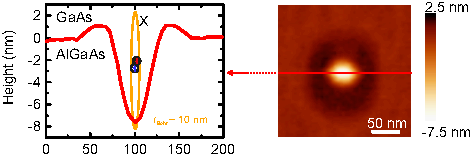
\includegraphics[width=0.9\linewidth]{figures/quantum-dot/QD_plot_AFM}
	\caption{Height profile (red) of a droplet-etched nanohole in an AlGaAs layer is shown in the left image.
	The orange line represents the wavefunction of the exciton which resembles the ground state of an hydrogen atom.
	Because of that the bohr radius $r_{\textrm{Bohr}}$ is denoted.
	The right image shows the atomic force microscopy picture of the nanohole.
	An GaAs quantum dot is obtained after filling the hole with GaAs and avergrowth with AlGaAs~\cite{reindl_highly_2019}}
	\label{fig:qdplotafm}
\end{figure}

\section{Adiabatic rapid passage}

\section{Fine structure splitting}


\section{Exciton emission spectrum}

The discussion of the emission of GaAs quantum dots in the following chapters will be limited to excitonic emission. 
This section will provide the basis for chapter~\ref{chapter:scanning-fabry-perot}.

\subsection{Zero-phonon line and phonon sideband}

\todo{\url{https://en.wikipedia.org/wiki/Zero-phonon_line_and_phonon_sideband}}

\subsection{Calculate spectral range of zero-phonon line}
A typical lifetime of a GaAs quantum dot is $\Delta t = 250~ps$.
According to the time-energy uncertainty relation
\begin{align}
\Delta E \cdot \Delta t = \frac{h}{2 \pi}\\
\Rightarrow \Delta E = \SI{2.64}{\micro \electronvolt}
\end{align}
The frequency uncertainty can be obtained through
\begin{equation}
\Delta \nu = \frac{\Delta E}{h}
\end{equation}
By developing $\lambda$into a taylor series
\begin{align}
\label{eq:planck-einstein}
\lambda &= \frac{c}{\nu}\\
\Rightarrow \lambda(\nu) &\approx \lambda(\nu_0) + \lambda'(\nu_0) \cdot (\nu - \nu_0)
\end{align}
$\Delta \lambda$ can be expressed as
\begin{align}
\Delta \lambda &= \lambda(\nu_0 - \Delta \nu) - \lambda(\nu_0)\\
 &= \lambda(\nu_0) - \lambda'(\nu_0)\cdot\Delta \nu - \lambda(\nu_0)\\
 &= - \lambda'(\nu_0)\cdot \Delta \nu.
\end{align}
With equation~\eqref{eq:planck-einstein} this gives
\begin{align}
\Rightarrow \Delta \lambda &= \frac{c}{\nu_0^2} \cdot \Delta \nu = \frac{\lambda_0^2}{c}\cdot\Delta \nu\\
\label{eq:zero-phonon-theoretical-limit}
&\approx \SI{1.0}{\pico \metre}
\end{align}

\subsection{Simulation}

\begin{table}[H]
	\caption[Paramters of GaAs quantum dots used in the laboratory of semiconductor physics department in Linz.]{Parameters of GaAs quantum dots used in the laboratory of semiconductor physics department in Linz.
	Zero-phonon line calculates from from the theoretical limit according to the life time of the excitonic state (as can be seen in equation~\eqref{eq:zero-phonon-theoretical-limit}) up to broader lines which are still valued enough to be measured.
	The phonon sideband resembles data taken from \textcite{scholl_resonance_2019}.}
	\label{tab:quantum-dot-emission}
	\begin{tabular}{@{}llll@{}}
		\toprule
		Quantum dot emission & Center wavelength $\lambda_0$           & Spectral range $\Delta \lambda$ & Waveform                  \\ \midrule
		Zero-phonon line               & \SIrange{700}{800}{\nano \metre} & \SIrange{1.0}{1.4}{\pico \metre} & Cauchy\\
		Phonon sideband       & \SI{\sim 0.25}{\nano \metre} higher than zero-phonon line  & ~\SI{500}{\pico \metre} & Gauss  \\ \bottomrule
	\end{tabular}
\end{table}

The zero-phonon line is described with a Cauchy distribution
\begin{equation}
\Phi_{dot,zero}(\lambda) = \frac{1}{\pi \cdot \Delta\lambda_{zero} \cdot 0.5 \left[1+\left(\frac{\lambda - \lambda_{0, zero}}{\Delta\lambda_{zero} \cdot 0.5}\right)^2\right]}
\end{equation}
with $\lambda_{0, zero}$ as the center wavelength and $\Delta\lambda_{zero}$ as the spectral range of the zero-phonon line.

The phonon side band is described with a Gauss distribution
\begin{equation}
\Phi_{dot,side}(\lambda) = \frac{1}{\sqrt{2\cdot\pi\cdot \Delta\lambda_{side}^2}}\cdot exp\left(-\frac{(\lambda - \lambda_{0, side})^2}{2\cdot \Delta\lambda_{side}^2}\right)
\end{equation}
with $\lambda_{0, side}$ as the center wavelength and $\Delta\lambda_{side}$ as the spectral range of the phonon side band.

\begin{figure}[H]
	\centering
	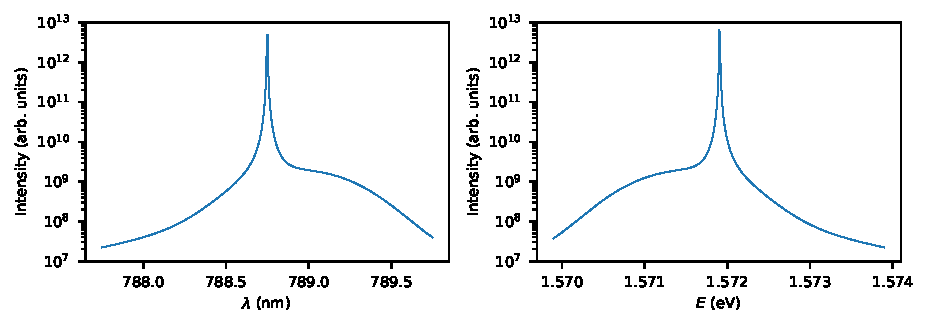
\includegraphics{figures/fabry-perot/plots/quantum_dot_emission_wavelength_energy}
	\caption[Simulated exciton emission of a GaAs quantum dot]{Simulated exciton emission of a GaAs quantum dot plotted dependant on the wavelength $\lambda$ and the Energy $E$.
		The parameters can be found in table~\ref{tab:quantum-dot-emission}.}
	\label{fig:quantumdotemissionwavelengthenergy}
\end{figure}


Dot-Spectra in far field is (TEM$_{00}$).




% !TEX root = ../masterthesis.tex
\chapter{Methods}

\todo{Einleitung}


\section{Optical setup}

The setup used for the measurements described in following chapters is sketched in figure~\ref{fig:setupflat}.

\begin{figure}[H]
	\centering
	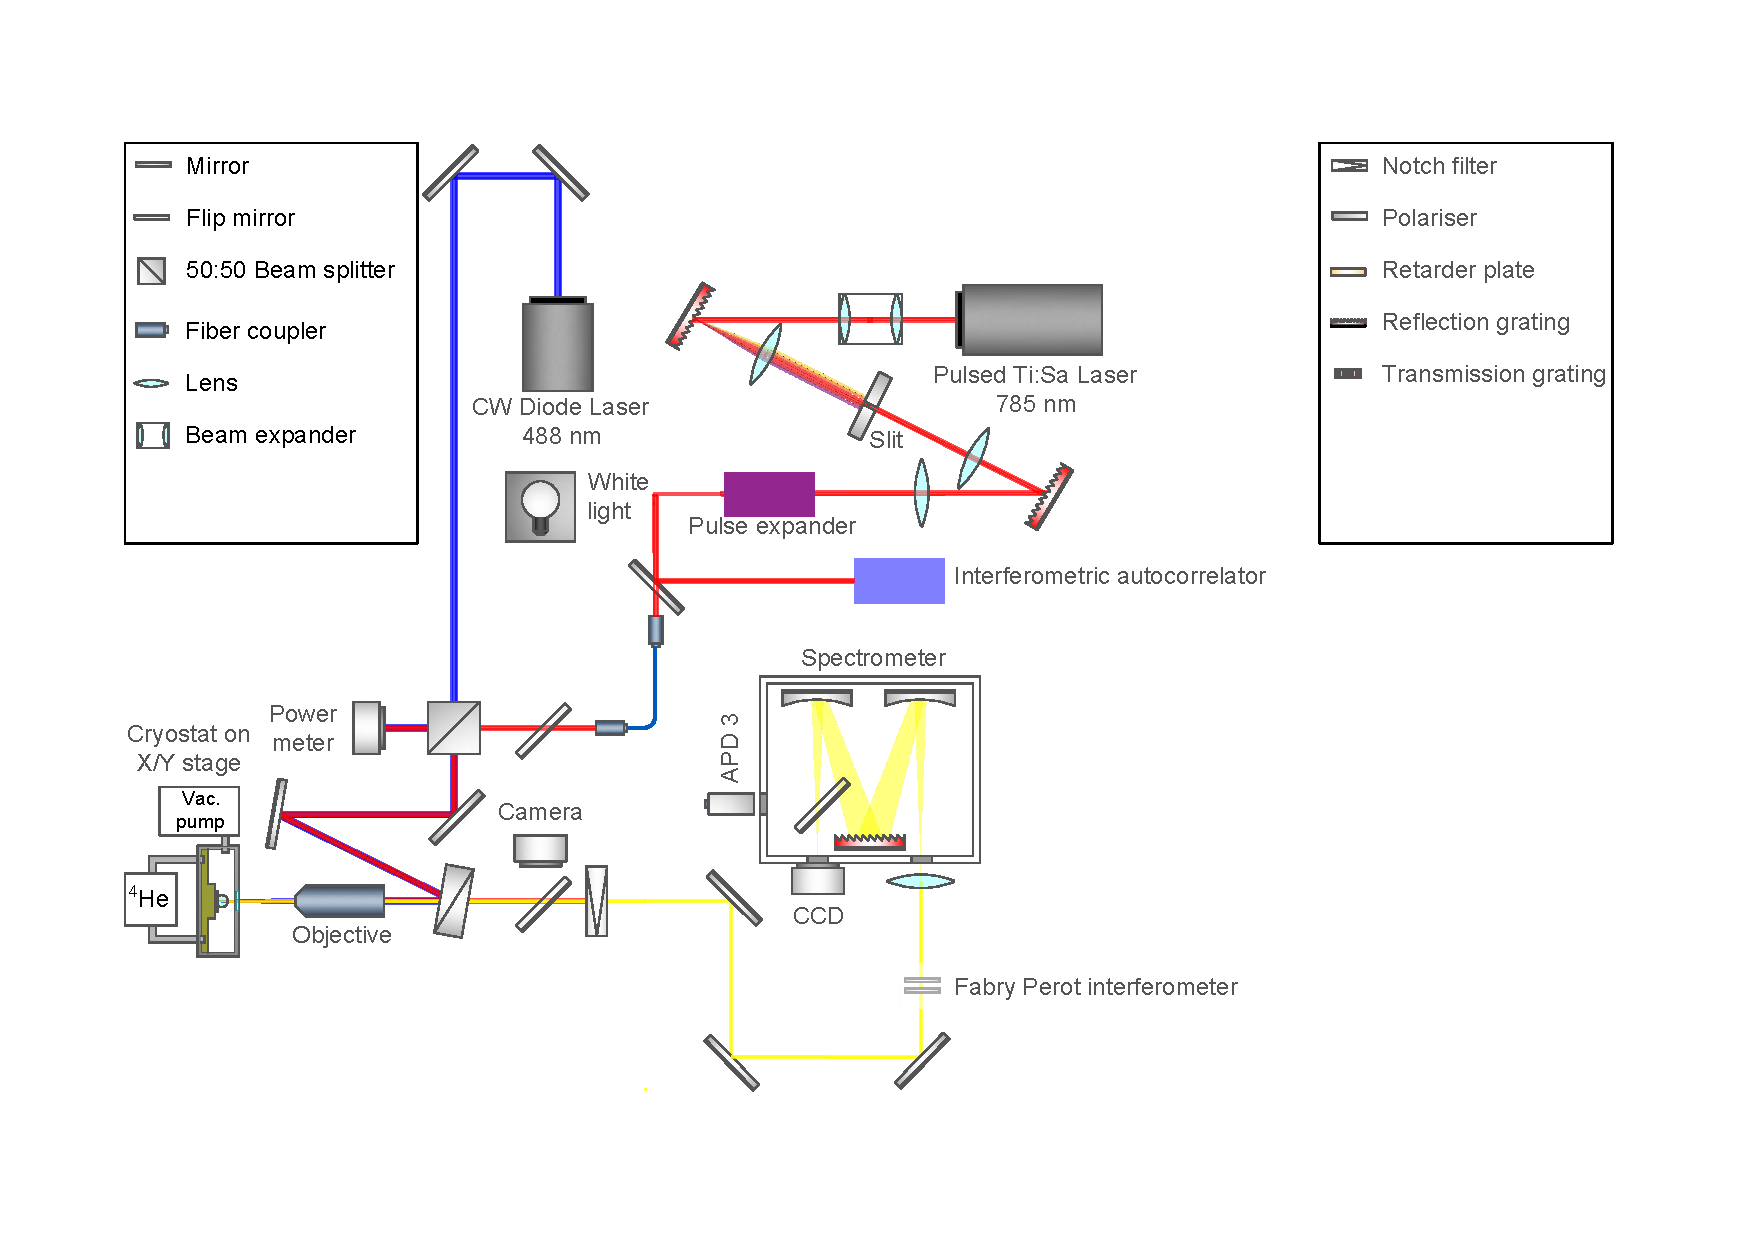
\includegraphics[width=\linewidth]{figures/setup/Setup_flat}
	\caption[Complete experimental setup]{Complete experimental setup, which was used in order to quantify the chirp of the Ti:Sa Laser and resolve spectral emission of a quantum dot~\cite{schimpf_towards_2017}.}
	\label{fig:setupflat}
\end{figure}

\todo{Pulse shaper 4F geometrie, florian sipek}

Pulse shaper~\cite{sipek_spectral_2016}.

\section{Micro photo-luminescence}
\begin{figure}[H]
	\centering
	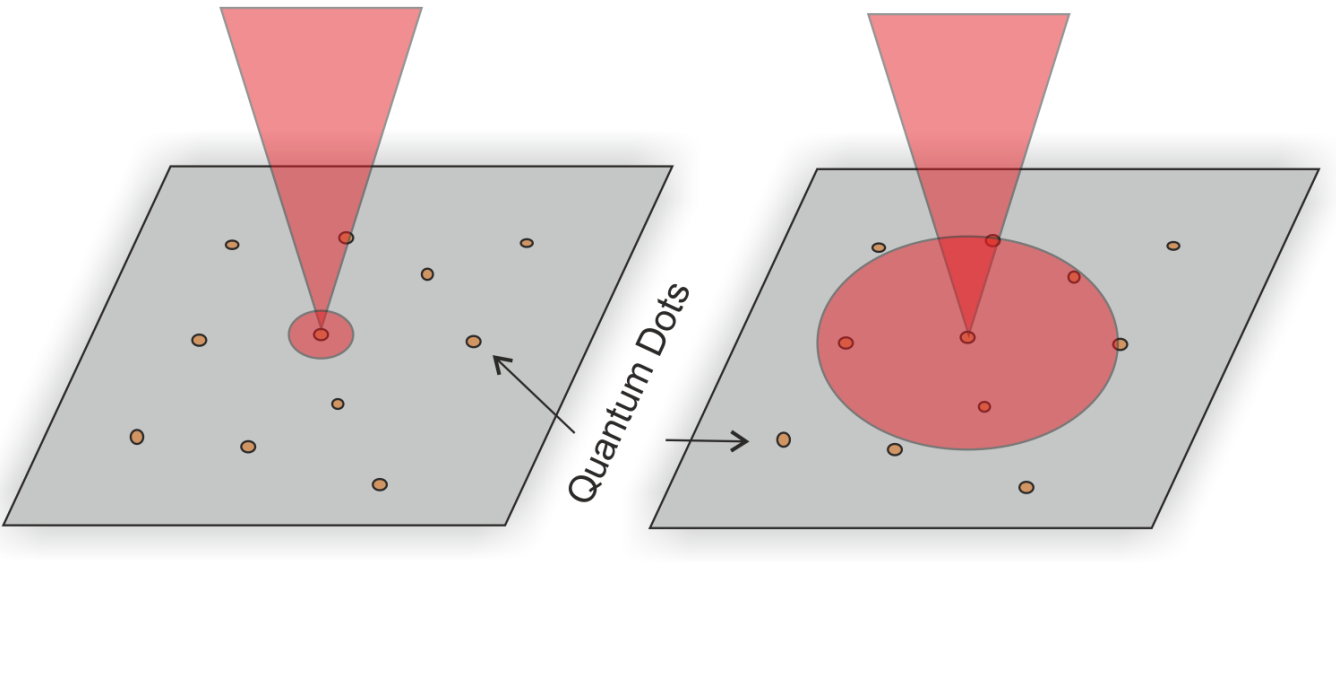
\includegraphics[width=0.7\linewidth]{figures/setup/micro-pl}
	\caption{Laser beam of different spot sizes illuminating quantum dots~\cite{reindl_characterisation_2014}.}
	\label{fig:micro-pl}
\end{figure}
The following chapters will investigate the optical properties of \ac{QD}.
In order to achieve that, it is necessary to excite and collect light of only a single one.
This is achieved by \ac{MPL}, which involves (i) reducing the diameter of the excitation laser beam and (ii) using samples with a low \ac{QD} density~\cite{reindl_characterisation_2014}.
(i) can be improved by using an objective, where its minimal achievable spot size $d$ is described by
\begin{equation}
d = \frac{\lambda}{2 \cdot NA}
\end{equation}
with $NA$ as the numerical aperture.
As the wavelength of the laser $\lambda$ is adjusted according parameter of the \ac{QD}, $NA$ is the adjustable factor.
In our laboratory, an objective of $NA=0.62$ is used, allowing laser spot sizes in the order of the excitation wavelength.
A \ac{QD} density of $\approx 1 / \lambda^2$ is therefore necessary in order to examine single \ac{QD} emission.

The sample containing the \acp{QD} is mounted inside the cryostat, which is cooled down to \SI{4}{\kelvin}.
This is necessary as the influence of dephasing processes increases with higher temperature due to carrier-phonon interaction.
The laser beam is then focused on the sample by the objective and the \ac{QD} emission is then collected by the very same objective and passed through a beam splitter.
% !TEX root = ../masterthesis.tex
\chapter{Entangled photon generation using adiabatic rapid passage with frequency-chirped pulses}
\label{cha:chirp}

\section{Introduction and motivation}

In order to efficiently use the biexciton decay cascade, the \acl{XX} state has to be prepared beforehand in a robust way.
This chapter deals with the efficient inversion of the \ac{QD} from the ground state to the biexciton level via \ac{ARP}.
\acs{ARP} uses chirped pulses, which need to be measured and deterministically adjusted in order to effectively use them.
Therefore, the majority of this chapter will focus on the chirp and how to determine and adjust it, with the help of simulations and later with measurements.


\section{Chirp}
\label{sec:chirp}
A chirped signal is a signal whose frequency changes over time.
For example, the frequency of a linearly chirped signal $f(t)$ would be described by
\begin{equation}
f(t) = ct+f_0
\end{equation}
where $f_0$ is the starting frequency at $t=0$ and $c$ is the chirpyness. A linearly chirped sinusoidal wave is depicted in figure~\ref{fig:chirped-sin}.

\begin{figure}[H]
	\centering
	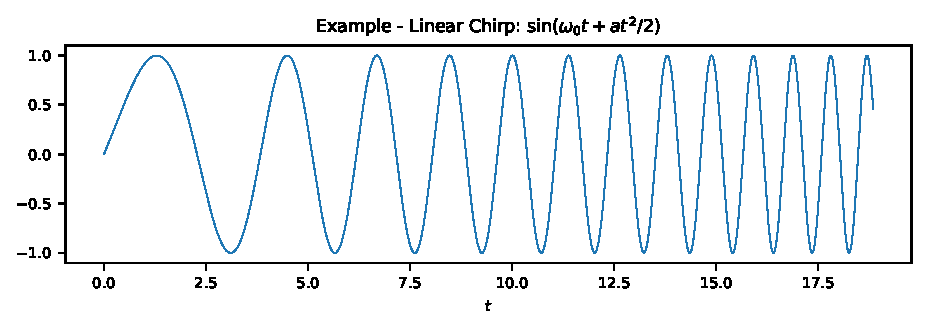
\includegraphics[width=\linewidth]{figures/chirp/plots/chirped-sin}
	\caption{A chirped sinusoidal wave which increases in frequency over time.}
	\label{fig:chirped-sin}
\end{figure}

As this chapter is concentrated on exciting \acp{QD} with frequency-chirped pulses, the mathematical description of chirped laser pulses will now be discussed. The shape of the electric field of a laser $E(t)$ can be approximated by
\begin{equation}
\label{eq:electric-field-laser}
E(t) \sim \mathrm{Re}\left(f^{1/2}(t) \cdot \exp\left(-i \omega t - i \phi(t)\right)\right)
\end{equation}
with the central frequency $\omega$ and the linear chirp $\phi(t)$.

Depending on the laser either a Gaussian or a hyperbolic secant describes the pulse shape more accurately~\cite{glassl_biexciton_2013, hirayama_real-time_2002}

\begin{itemize}
	\item Gaussian pulse:
	\begin{itemize}
		\item Pulse shape of
		\begin{equation}
		\label{eq:f_gauss}
		f_{gauss}(t) = \left(\frac{A_{gauss}}{\sqrt{2 \cdot \pi \cdot \tau_0 \cdot \tau}} \exp\left(-\frac{t^2}{2 \cdot \tau^2}\right)\right)^2
		\end{equation}
		with the normalization constant $A_{gauss}$, the pulse duration $\tau_0$, the central frequency $\omega$ and the chirp coefficient $\alpha$.
		\item Linear chirp of
		\begin{equation}
		\label{eq:phi-gauss}
		\phi_{gauss}(t) = \frac{a_{gauss} t^2}{2}
		\end{equation}
		where 
		\begin{equation}
		\tau = \sqrt{\alpha^2 / \tau_0^2 + \tau_0^2}
		\end{equation}
		characterizes the chirped pulse length and
		\begin{equation}
		\label{eq:chirp-parameter}
		a = \alpha / (\alpha ^ 2 + \tau _0 ^ 4)
		\end{equation}
		is the frequency chirp rate.
	\end{itemize}
	\newpage
	\item Secant pulse:
	\begin{itemize}
		\item Pulse shape of
		\begin{equation}
		f_{secant}(t) = A_{secant} \cdot \textrm{sech}^2\left(\frac{t}{\tau_0}\right) = A_{secant} \cdot \left(\frac{2}{\exp(\frac{t}{\tau_0}) + \exp(-\frac{t}{\tau_0})}\right)^2
		\end{equation}
		with the normalization constant $A_{secant}$, the pulse duration $\tau_0$, the central frequency $\omega$ and the chirp coefficient $\alpha$.
		\item Linear chirp of
		\begin{equation}
		\phi_{secant}(t) = \alpha_{secant}\left(\frac{t}{\tau_0}\right)^2
		\end{equation}
	\end{itemize}
\end{itemize}

The following discussion will assume a Gaussian laser shape as described by equation~\eqref{eq:f_gauss} and \eqref{eq:phi-gauss}.
A simulation for $E$ is plotted in figure~\ref{fig:chirpedlaserpulse} for different chirp parameters $\alpha$ suitable to display examples for strong and weak chirps.
As can be seen there, the chirp parameter strongly influences the shape of the electric field.
If $E$ could be measured directly, the chirp could be easily estimated.
This is not feasible in our case, as our Ti:Sa laser can produce laser pulses as short as \SI{100}{\femto \second} and response times of photodiodes and oscilloscopes are in the best case in the order of \SI{200}{\femto \second}.
This means they cannot even measure the duration of these ultrashort pulses let alone resolve the pulse shape.

\begin{figure}[H]
	\centering
	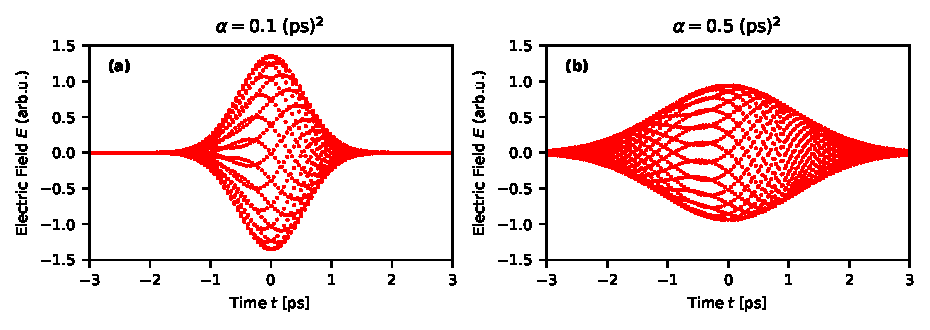
\includegraphics[width=\linewidth]{figures/chirp/plots/chirped_laser_pulse}
	\caption{Electric field $E$ of Gaussian laser pulse of pulse duration $\tau_0=\SI{0.5}{\pico \second}$ for chirp of (a) $\alpha = \SI{0.1}{\pico \second \squared}$ and (b) $\alpha = \SI{0.5}{\pico \second \squared}$}
	\label{fig:chirpedlaserpulse}
\end{figure}

\newpage

\section{Measuring the chirp with interferometric autocorrelation}
\begin{figure}[H]
	\centering
	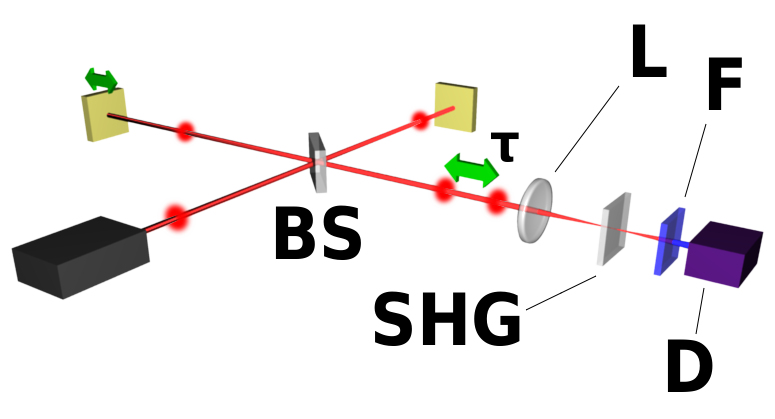
\includegraphics[width=0.6\linewidth]{figures/chirp/Optical-interferometric-autocorrelation-setup.png}
	\caption[Schematics of an interferometric autocorrelator]{Schematics of an interferometric autocorrelator, where \textbf{L} is a converging lens, \textbf{SHG} a second-harmonic generation crystal, \textbf{BS} a beam splitter, \bm{$\tau$} the interval between two pulses, \textbf{D} the detector and \textbf{F} a spectral filter to block the fundamental wavelength~\cite{noauthor_optical_nodate}.}
	\label{fig:optical-field-autocorrelation-setup}
\end{figure}
In order to estimate the pulse width $\tau_0$, \ac{IAC} is used.
Basically, a nonlinear crystal is added to a Michelson interferometer in order to generate a signal governed by
\begin{equation}
\label{eq:i-m-integral}
I_M(\tau) = \int_{-\infty}^{+\infty}\langle|(E(t)+E(t-\tau))^2|^2\rangle dt.
\end{equation}
and plotted in figure~\ref{fig:imgausschirpwithoutslitwithoutmosaic}~\cite{diels_ultrashort_2006}.
Here, $\langle \rangle$ denotes averaging over fast oscillations of the electric field.
\begin{figure}[H]
	\centering
	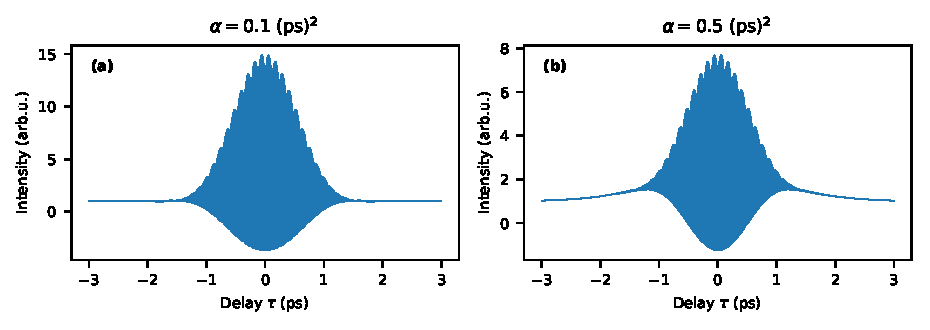
\includegraphics[width=\linewidth]{figures/chirp/plots/I_M_gauss_chirp_without_slit_without_MOSAIC}
	\caption{Intensity of IAC of a Gaussian laser pulse of pulse duration $\tau_0=\SI{0.5}{\pico \second}$ without applied MOSAIC filter for chirp of (a) $\alpha = \SI{0.1}{\pico \second \squared}$ and (b) $\alpha = \SI{0.5}{\pico \second \squared}$}
	\label{fig:imgausschirpwithoutslitwithoutmosaic}
\end{figure}
Under the use of equation~\ref{eq:electric-field-laser}, equation~\eqref{eq:i-m-integral} can be expanded to
\begin{align}
I(\tau) = 1 &+ 2 \int f(t) f(t + \tau) dt + \int f(t) f(t + \tau) \cos(2 \omega \tau + 2 \Delta \phi) dt \nonumber\\
&+ 2 \int f^{1/2}(t) f^{3/2}(t + \tau) \cos(\omega \tau + \Delta \phi) dt + 2 \int f^{3/2}(t) f^{2/2}(t + \tau) \cos(\omega \tau + \Delta \phi) dt
\end{align}
where $\Delta \phi(t, \tau) = \phi(t + \tau) - \phi(t)$ and $\int f(t) dt = 1$.

As can be seen in figure~\ref{fig:imgausschirpwithoutslitwithoutmosaic}, the chirp parameter $\alpha$ has hardly any measurable influence on the resulting signal.
However, certain modifications to the \ac{IAC} signal introduced by \textcite{hirayama_real-time_2002} make it much more sensitive to the temporal chirp.
It is called \ac{MOSAIC} and performs the following transformations on the \ac{IAC} spectrum: The $\omega$ terms are eliminated and the $2\omega$ term is doubled.
The \ac{MOSAIC} signal is then described by
\begin{equation}
\label{eq:i-m-filtered}
I_{M}(\tau) = 1 + 2 \int f(t) f(t + \tau) dt + 2 \int f(t) f(t + \tau) \cos(2\omega \tau + 2\Delta \phi) dt.
\end{equation}
When the MOSAIC filter is applied to the data in figure~\ref{fig:imgausschirpwithoutslitwithoutmosaic}, this results in a signal as shown in figure~\ref{fig:mosaicchirpedlaserpulse}.
Here the influence of the chirp is clearly visible in the lower envelope.
\begin{figure}[H]
	\centering
	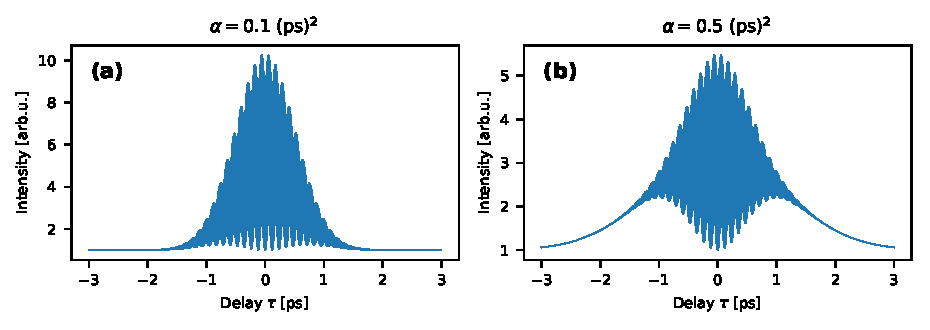
\includegraphics[width=\linewidth]{figures/chirp/plots/mosaic_chirped_laser_pulse}
	\caption{Intensity of IAC of a Gaussian laser pulse of pulse duration $\tau_0=\SI{0.5}{\pico \second}$ for chirp of (a) $\alpha = \SI{0.1}{\pico \second \squared}$ and (b) $\alpha = \SI{0.5}{\pico \second \squared}$}
	\label{fig:mosaicchirpedlaserpulse}
\end{figure}

\newpage

The points of the lower envelope can be obtained by determining the local minima of the signal as shown in figure~\ref{fig:mosaicchirpedlaserpulsefindenvelope}.

\begin{figure}[H]
	\centering
	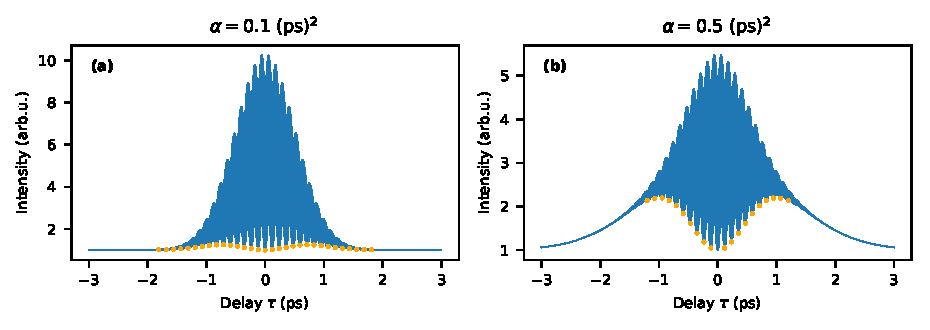
\includegraphics[width=\linewidth]{figures/chirp/plots/mosaic_chirped_laser_pulse_find_envelope}
	\caption{Intensity of IAC of a Gaussian laser pulse of pulse duration $\tau_0=\SI{0.5}{\pico \second}$ with applied MOSAIC filter for chirp of (a) $\alpha = \SI{0.1}{\pico \second \squared}$ and (b) $\alpha = \SI{0.5}{\pico \second \squared}$.
		The orange dots are results of a numerical peak finder algorithm, executed in order to find local minima.}
	\label{fig:mosaicchirpedlaserpulsefindenvelope}
\end{figure}

The lower bound (minima envelope) of the MOSAIC trace can be derived by use of a standard textbook procedure~\cite{klein_optics_1986}
\begin{equation}
S^{min}_{MOSAIC}(\tau)= 1 + 2 \cdot g(\tau) - 2 \cdot [g_s^2(\tau)+g_c^2(\tau)]^{1/2}
\end{equation}
with
\begin{align}
g(\tau)&=\int f(t)f(t+\tau)dt\\
g_s(\tau)&=\int f(t)f(t+\tau)sin(2\Delta\phi)dt\\
g_c(\tau)&=\int f(t)f(t+\tau)cos(2\Delta\phi)dt.
\end{align}
The points of the lower envelope determined before can now be fitted in order to obtain the chirp parameter $\alpha$ as shown in figure~\ref{fig:mosaicchirpedlaserpulsefitenvelope}.
It is visible that the fitted values of $\alpha$ correspond to the expected values.
\begin{figure}[H]
	\centering
	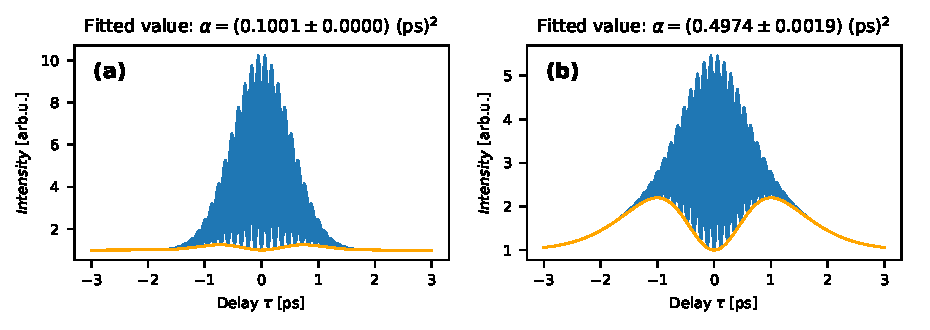
\includegraphics[width=\linewidth]{figures/chirp/plots/mosaic_chirped_laser_pulse_fit_envelope}
	\caption[Intensity of IAC of a Gaussian laser pulse of pulse duration $\tau_0=\SI{0.5}{\pico \second}$ with applied MOSAIC filter and fitted $\alpha$-values.]{Intensity of IAC of a Gaussian laser pulse of pulse duration $\tau_0=\SI{0.5}{\pico \second}$ with applied MOSAIC filter for chirp of (a) $\alpha = \SI{0.1}{\pico \second \squared}$ and (b) $\alpha = \SI{0.5}{\pico \second \squared}$.
		The orange line is a fit for the lower envelope of the MOSAIC signal in order to obtain~$\alpha$.}
	\label{fig:mosaicchirpedlaserpulsefitenvelope}
\end{figure}

\section{Deterministically adjusting the chirp with a pulse expander}
\label{sec:pulse-expander}
\begin{figure}[H]
	\centering
	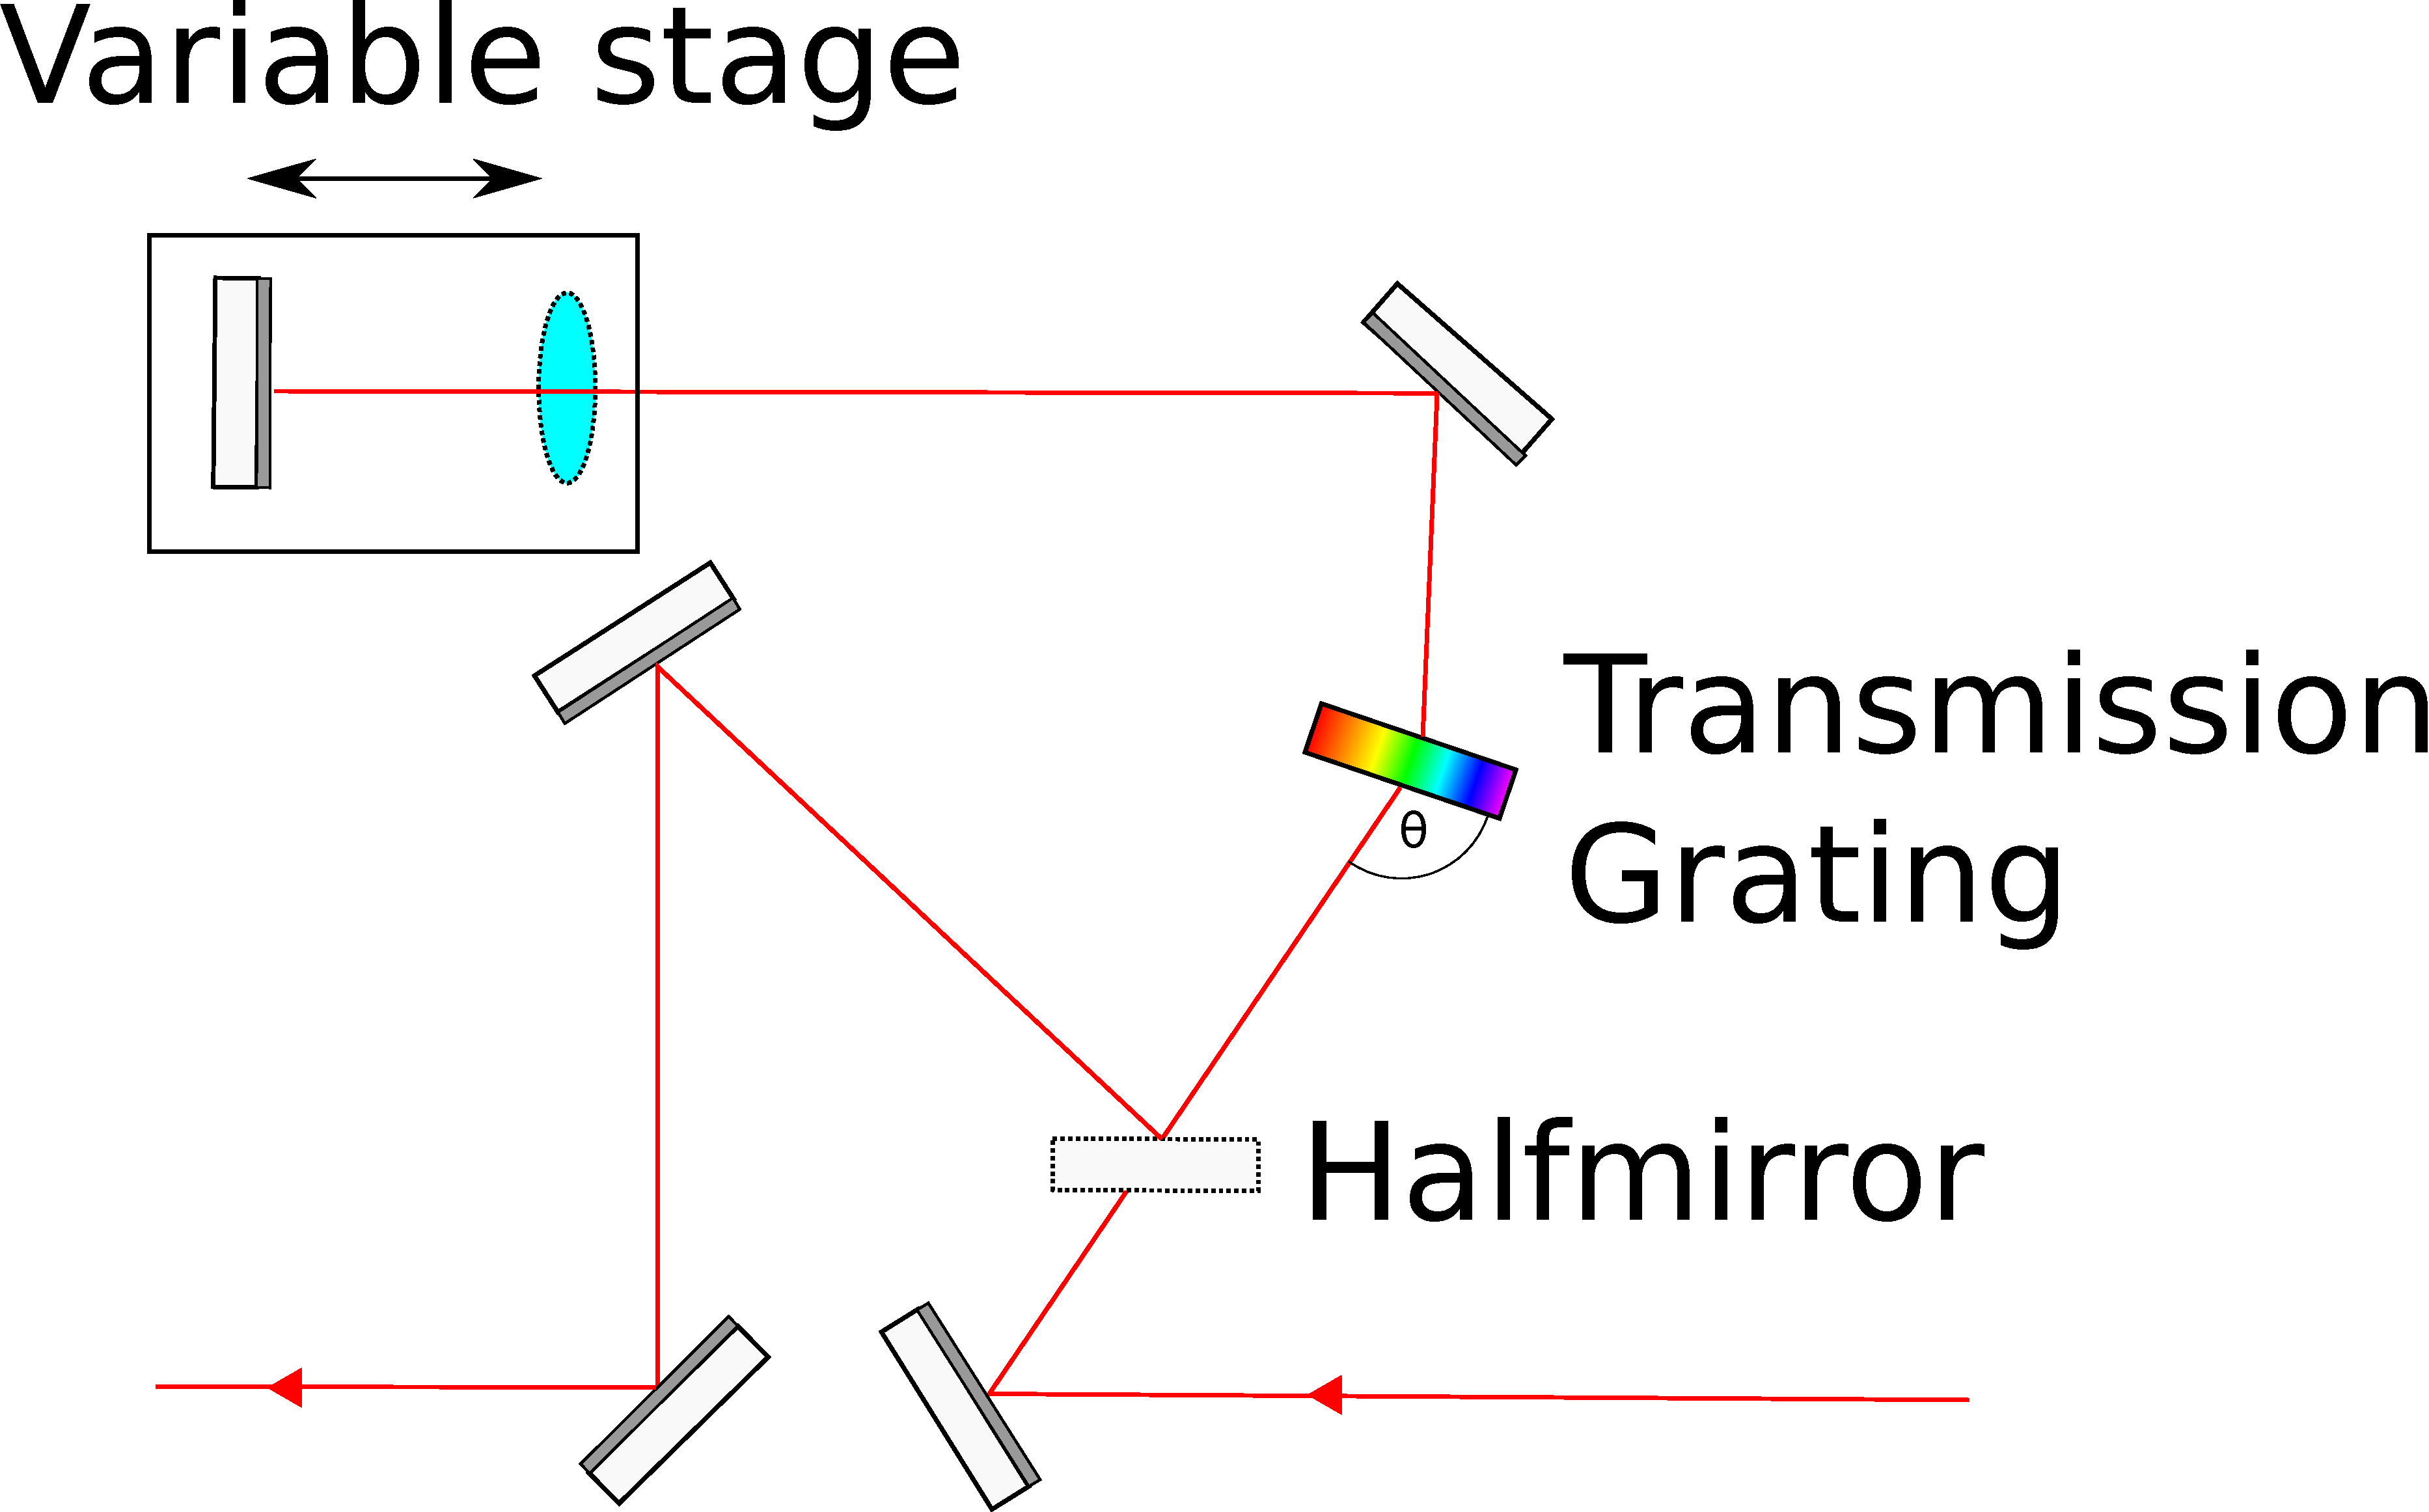
\includegraphics[width=0.7\linewidth]{figures/chirp/pulse-expander}
	\caption{Scheme of a folded pulse expander as described by \textcite{martinez_3000_1987}.
		The light enters on the right side, passes the halfmirror, and enters the system of transmission grating, lens and mirrors.
		Afterwards it hits the halfmirror and exits on the left hand.
		It induces an accumulated group velocity dispersion on the signal depending on the optical distance between the transmission grating and the lens.}
	\label{fig:pulse-expander}
\end{figure}



In the optimal case the chirp of the pulse can be deterministically adjusted in order to most efficiently excite the \ac{QD} via adiabatic rapid passage (going to be introduced in section~\ref{sec:arp}).
Grating compressors as discussed by \textcite{martinez_3000_1987} were originally used to compensate the broadening effect fibers have on pulses.
However, together with a telescope they have the inverse effect and can be used to induce a chirp.
A setup like this is sketched in figure~\ref{fig:pulse-expander} and it will in future references in this work be called \textit{pulse expander}.
Its main elements are a transmission grating and a lens.
This folded setup uses a mirror after the lens in order to need only one lens and mirror.
The accumulated group velocity dispersion $\frac{d^2 \Phi}{d \omega^2}$ can be adjusted by varying the optical distance $d$ between the focal plane of the lens and the transmission grating and is described by
\begin{equation}
\frac{d^2 \Phi}{d \omega^2} = k \beta^2 2 d
\end{equation}
where $k$ is the wavenumber and $\beta$ is given by
\begin{equation}
\beta = \frac{\lambda}{2 \pi \omega_0 \cos \theta}
\end{equation}
with $\lambda$ denoting the centre wavelength, $w_0$ the beam waist (beam size at the point of its focus) and $\theta$ the emerging angle as sketched in figure~\ref{fig:pulse-expander}.

\begin{figure}[H]
	\centering
	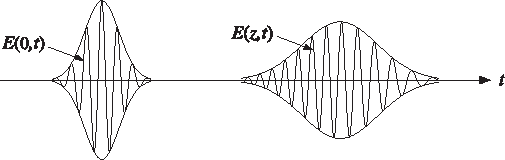
\includegraphics[width=0.7\linewidth]{figures/chirp/group-velocity-dispersion}
	\caption{Influence of group velocity dispersion for example inside a fiber on a Gaussian pulse~\cite{orfanidis_electromagnetic_2002}}
	\label{fig:group-velocity-dispersion}
\end{figure}

As can be seen in figure~\ref{fig:group-velocity-dispersion}, a group velocity dispersion has a similar effect on a Gaussian pulse as a chirp.
In fact, the frequency chirp rate $a_{gauss}$ introduced in equation~\eqref{eq:phi-gauss} can be put into relation with it by:~\cite{orfanidis_electromagnetic_2002}
\begin{equation}
a_{gauss} = \frac{\frac{d^2 \Phi}{d \omega^2}}{\tau_0^4 + \left(\frac{d^2 \Phi}{d \omega^2}\right)^2}
\end{equation}



\section{Adiabatic rapid passage}
\label{sec:arp}
One way to invert the \ac{QD} from the ground state $\ket{G}$ to the biexciton state $\ket{XX}$ is by exciting it with a narrow-band laser pulse of constant centre frequency, which equals to half of the ground state biexciton transition frequency.
As described in equation~\eqref{eq:n-xx}, if the pulse area $\theta=\pi$, a population inversion from the $\ket{G}$ state to the $\ket{XX}$ occurs.
However, the $\pi$-pulse method is not a generally robust scheme.
In order to ensure the inversion, precise control of the field intensity is required~\cite{glassl_biexciton_2013}.
Adiabatic rapid passage \acused{ARP} (\acs{ARP}) with frequency chirped pulses is a much more robust alternative to this Rabi-flopping scheme.
Here, the frequency of the laser signal is swept through resonance, starting slightly above or below the resonance frequency.
The biexciton state can be populated with nearly perfect efficiency~\cite{glassl_biexciton_2013} if the process is performed adiabatically, i.e. if~\cite{malinovsky_general_2001}
\begin{equation}
\Omega_0^2 \gg |\frac{d}{dt} \omega(t)|
\end{equation}
where $\Omega_0$ is the peak Rabi frequency and $\omega(t)$ is the center frequency of the laser pulse. 

In figure~\ref{fig:biexciton-occupation} simulations in order to determine the final biexciton occupation for different biexciton binding energies $\Delta$ by \textcite{glassl_biexciton_2013} are presented.
Here, a linearly-chirped Gaussian laser pulse as discussed in section~\ref{sec:chirp} was assumed.
\begin{figure}[H]
	\centering
	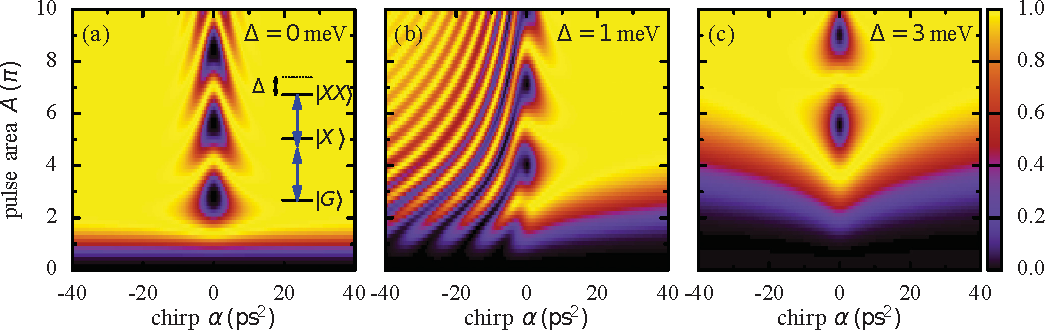
\includegraphics[width=\linewidth]{figures/chirp/biexciton-occupation}
	\caption[Final biexciton occupation after chirped Gaussian pulse of pulse duration $\tau_0 = \SI{2}{\pico \second}$]{Final biexciton occupation after chirped Gaussian pulse of pulse duration $\tau_0 = \SI{2}{\pico \second}$.
		It is plotted against the original pulse area $A$ (vertical axis) and the chirp parameter $\alpha$ for biexciton binding energies of (a) $\Delta=0$, (b) 1, and (c) \SI{3}{\milli \electronvolt}~\cite{glassl_biexciton_2013}.}
	\label{fig:biexciton-occupation}
\end{figure}
The central frequency is chosen so that for $\alpha=0$ it resonates to groundstate-to-biexction transition, which is sketched in figure~\ref{fig:biexciton-occupation}.
For $\alpha=0$ Rabi oscillations are visible and their period depends strongly on the biexciton binding energy $\Delta$.
However, for $\alpha \gg 0$ biexciton preparation becomes insensitive to small variations of the pulse area $A$ as long it exceeds a certain threshold.
This is therefore the regime which would be the most suitable to work in.
In the case of $\alpha < 0$ this insensitivity does not appear for moderate values of $\Delta$ as can be seen in figure~\ref{fig:biexciton-occupation}(b).

\newpage
\section{Measurements and discussion}
As discussed in the sections above, the final goal is to excite a \ac{QD} via \ac{ARP}.
The first step to do that is to determine the chirp of a laser pulse which only passed the pulse shaper with the \ac{IAC}.
Here a laser pulse of only $\tau_0=\SI{344}{\femto \second}$ was used as the \ac{IAC} can not resolve fine enough details for greater $\tau_0$.
Even though broader peaks will be necessary in order to excite the \ac{QD} with \ac{ARP}, this is not a problem as the equivalent chirp can be calculated for greater $\tau_0$ with equation~\eqref{eq:chirp-parameter}.

Afterwards, a signal was measured after passing a pulse expander as discussed in section~\ref{sec:pulse-expander} and sketched in figure~\ref{fig:setupflat}.
The comparison between these two is shown in figure~\ref{fig:measuredchirpedlaserpulsebeforemosaic}.
Compared to the simulations in figure~\ref{fig:imgausschirpwithoutslitwithoutmosaic} it is visible that the \ac{IAC} of the laser pulse without the pulse expander fits the expected shape well, while the one with the pulse expander does not.
Possible reasons could be that the chirp is too high for the model used in the simulation to work or that the pulse expander introduces side effects not considered in the simulation.

\begin{figure}[H]
	\centering
	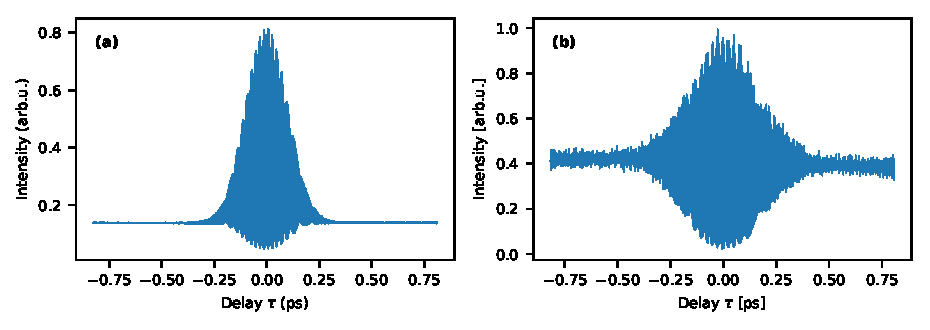
\includegraphics[width=\linewidth]{figures/chirp/plots/measured_chirped_laser_pulse_before_MOSAIC}
	\caption{Measured IAC of Ti:Sa Laser without (a) and with (b) pulse expander before the autocorrelator.}
	\label{fig:measuredchirpedlaserpulsebeforemosaic}
\end{figure}

The same signals after applying the \ac{MOSAIC} filter are shown in figure~\ref{fig:measuredchirpedlaserpulseaftermosaic}.
It is visible that the lower envelopes in figure~\ref{fig:measuredchirpedlaserpulseaftermosaic}(a) and \ref{fig:measuredchirpedlaserpulseaftermosaic}(b) do not resemble the expected ones in figure~\ref{fig:mosaicchirpedlaserpulse}.
As the laser signal without pulse expander was assumed to be relatively unchirped, it is already unexpected that the lower envelope differs that much from a constant line at zero intensity.
One explanatory approach could be that the laser was already chirped to begin with. However, this would not explain why the shape of the lower envelope differs from the characteristic one of the simulation.
The next approach was to send the laser without pulse shaper into the \ac{IAC}.
However, the envelope of the signal after applying the \ac{MOSAIC} filter showed no visible difference to signal which has not passed a pulse shaper (depicted in figure~\ref{fig:measuredchirpedlaserpulseaftermosaic}).

\begin{figure}[H]
	\centering
	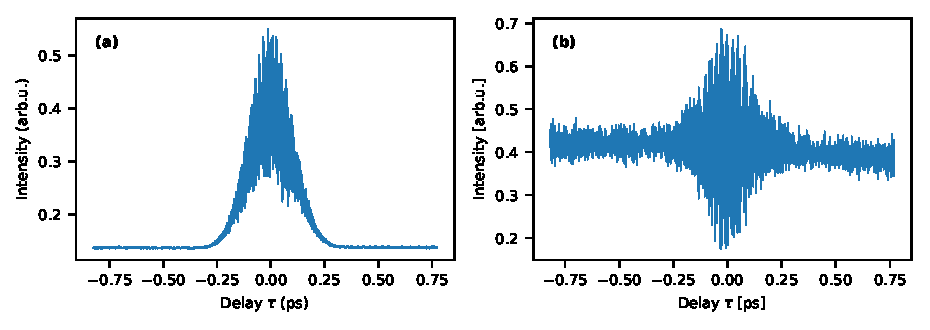
\includegraphics[width=\linewidth]{figures/chirp/plots/measured_chirped_laser_pulse_after_MOSAIC}
	\caption{Measured IAC of Ti:Sa Laser with applied MOSAIC filter without (a) and with (b) pulse expander before the autocorrelator.}
	\label{fig:measuredchirpedlaserpulseaftermosaic}
\end{figure}

The next step would have been to deterministically excite the \ac{QD} with \ac{ARP}.
However, it might be advisable to repeat the same procedure with another ultrashort pulsed laser before in order to rule out that our laser is already heavily chirped to begin with.
Alternatively, \ac{ARP} with the pulse expander can be attempted without measuring the chirp first and iteratively adjusting the lens-grating distance until the optimum is reached. 
% !TEX root = ../masterthesis.tex
\chapter{Building up a scanning Fabry-Pérot interferometer from scratch}
\label{chapter:scanning-fabry-perot}
\section{Introduction and motivation}

The \ac{FPI} is an optical resonator developed by Charles Fabry and Alfred Pérot.
An incoming light beam will only be transmitted through the resonator consisting of two semi-transparent mirrors if it fulfils the resonance condition.\cite{kaldewey_coherent_2017}.
The resonance frequencies can be changed by adjusting the mirror distance.
By measuring the intensity at the output of the \ac{FPI}, this can be used to resolve fine features of an electromagnetic spectrum, like e.g. the emitted light from the exciton-groundstate radiative decay described in section~\ref{sec:zero-phonon-side-band}.
The following chapter introduces basics of electromagnetic radiation, describes simulations performed to size the components of the \ac{FPI} and displays measurement techniques used to obtain the resolved exciton spectrum.

\section{Transverse modes of electromagnetic radiation}


\subsection{Gaussian beam}
\label{subsec:gaussian-beam}

In this chapter, light beams are described by the wave picture according to \textcite{meschede_optik_2008}.
They fulfil the Maxwell equations and therefore their electric field $\mathbf{E}(\mathbf{r},t)$  fulfils the wave equation
\begin{equation}
\label{eq:wave-equation}
\left(\nabla^2 - \frac{1}{c^2}\frac{\partial}{\partial t^2}\right)\mathbf{E}(\mathbf{r},t) = 0.
\end{equation}
Along the propagation direction $z$ a light beam behaves similarly to a plane wave with constant amplitude $A_0$ which is a known solution to the wave equation~\eqref{eq:wave-equation}
\begin{equation}
\label{eq:plain-wave}
E(z,t)=A_0e^{-i(\omega t - kz)}.
\end{equation}
However, far from its source light is expected to behave like a spherical wave
\begin{equation}
E(\mathbf{r},t)=A_0\frac{e^{-i(\omega t -\mathbf{kr})}}{|\mathbf{kr}|}.
\end{equation}
To get a better understanding of the propagation of light, only paraxial (near the z-axis) parts  of the spherical wave are considered.
Additionally, the wave is split into its longitudinal (z-axis) part and its transversal part and beams with axial symmetry are assumed, which only depend on a transversal coordinate $\rho$.
Under these circumstances $\mathbf{kr}$ can be replaced with $kr$ and because of $\rho<<r,z$ the Fresnel approximation can be applied:
\begin{equation}
\label{eq:e-field-after-fresnel-approximation}
E(\mathbf{r})=\frac{A(\mathbf{r})}{|\mathbf{kr}|}e^{i\mathbf{kr}}\simeq\frac{A(z,\rho)}{kz}\exp\left(i\frac{k\rho^2}{2z}\right)e^{ikz}
\end{equation}
with $r = \sqrt{z^2+\rho^2} \simeq z+\rho^2/2z$.

Equation~\eqref{eq:e-field-after-fresnel-approximation} resembles the plain wave in equation~\eqref{eq:plain-wave}, with the spacial phase transversal modulated by $\exp(ik\rho^2/2z)$.
Another spherical wave solution can be obtained by applying the following replacement ($z_0$ is a real number)
\begin{equation}
z \rightarrow q(z)=z-iz_0
\end{equation}
with $q(z)$ as the complex beam parameter.
Thereby, the fundamental (or TEM$_{00}$) Gaussian mode has been constructed
\begin{equation}
\label{eq:fundamental-gaussian-mode}
E(z,\rho)\simeq\frac{A_0}{kq(z)}\exp\left(i\frac{k\rho^2}{2q(z)}\right)e^{ikz}.
\end{equation}

The electric and magnetic fields of Gauss modes are transversal to its propagation direction.
These waveforms are called transversal electric and magnetic modes with indices $(m,n)$.
Its fundamental solution is the TEM$_{00}$-Mode, which is the most important one and will therefore be examined in more detail in the rest of this subsection.

By executing the replacement $q(z)\rightarrow z-iz_0$ explicitly the equation~\eqref{eq:fundamental-gaussian-mode} can be expressed as
\begin{equation}
\frac{1}{q(z)}=\frac{z+iz_0}{z^2+z_0^2}=\frac{1}{R(z)}+i\frac{2}{k\omega^2(z)},
\end{equation}
with new variables $z_0$, $R(z)$ and $\omega(z)$ being introduced.
With the decomposition of the Fresnel factors into real and imaginary part, two factors can be identified: one complex phase factor, which describes the curvature of the wavefronts and a real factor, which describes the envelope of the beam.
Therefore, the exponential in equation~\eqref{eq:fundamental-gaussian-mode} becomes
\begin{equation}
\exp\left(i\frac{k\rho^2}{2q(z)}\right) \rightarrow \exp\left(i\frac{k\rho^2}{2R(z)}\right)\exp\left(-\left(\frac{\rho}{\omega(z)}\right)^2\right)
\end{equation}
\begin{figure}[H]
	\centering
	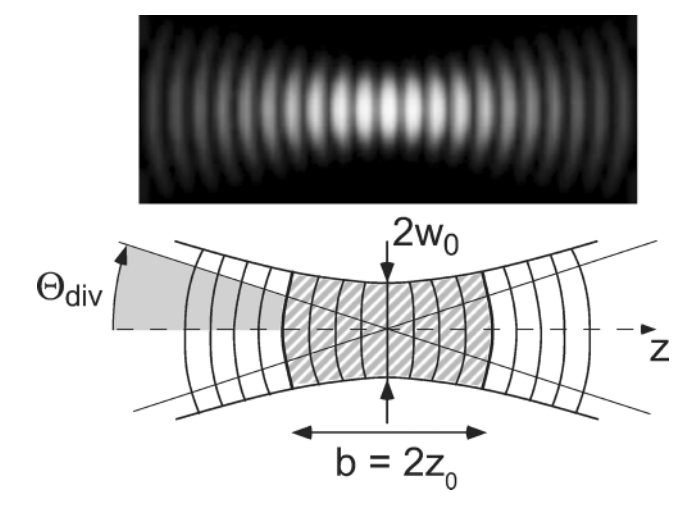
\includegraphics[width=0.8\linewidth]{figures/fabry-perot/gaussian-mode-near-beam-waist}
	\caption[A Gaussian beam near its beam waist.]
	{A Gaussian beam near its beam waist.
		Near the center they resemble plan wave fronts, while outside they converge towards spherical wave fronts.
		They Rayleighzone is shaded at the lower part of the figure.\cite{meschede_optik_2008}}
	\label{fig:gaussian-mode-near-beam-waist}
\end{figure}
For a proper description of a Gaussian beam as shown in figure~\ref{fig:gaussian-mode-near-beam-waist} the following  parameters have to be introduced
\begin{itemize}
	\item \textbf{Evolving radius of curvature} $R(z)$:
	\begin{equation}
	\label{eq:radius-wavefronts}
	R(z)=z(1+(z_0/z)^2)
	\end{equation}
	\item \textbf{Beam waist} $2\omega_0$:
	\begin{equation}
	\label{eq:beam-waist}
	\omega_0^2=\lambda z_0/\pi
	\end{equation}
\end{itemize}
The beam waist $2\omega_0$ or beam radius $\omega_0$ describes the smallest  beam cross section at $z=0$.
If the wave propagates inside a medium with the refractive index $n$, $\lambda$ has to be replaced with $\lambda/n$.
The cross section of the beam waist  is then $\omega_0^2=\lambda z_0/(\pi n)$.

A Gaussian beam can be completely characterized at every point $z$ on the beam axis either with the parameter couple $(\omega_0, z_0)$ or alternatively with the real and imaginary part of $q(z)$.
The parameters of the Gaussian beam are transformed by the ray transfer matrix
\begin{equation}
\label{eq:ABCD-rule}
q_{out}=\frac{A q_{in} + B}{C q_{in} + D}
\end{equation}
with the parameters $A, B, C, D$ determined by the optical element transforming the Gaussian beam described by $q_{in}$.

\subsection{Higher Gauss modes}
The wave equation~\eqref{eq:wave-equation} can be simplified by only allowing monochromatic waves with harmonic time dependence
\begin{equation}
\mathbf{E}(\mathbf{r},t) = \operatorname{Re}\left(\mathbf{E}(\mathbf{r})e^{-i\omega t}\right).
\end{equation}
With $\omega^2=c^2\mathbf{k}^2$, the \textit{Helmholtz equation} can be deduced, which only depends on the location \textbf{r}
\begin{equation}
\left(\nabla^2+\mathbf{k}^2\right)\mathbf{E}(\mathbf{r})=0.
\end{equation}
In favor of a formal treatment of the Gaussian modes, the Helmholtz equation is split into its transversal and longitudinal contributions,
\begin{equation}
\nabla^2+k^2=\frac{\partial^2}{\partial z^2} + \nabla_T^2+k^2
\quad\mathrm{with}\quad
\nabla_T^2=\frac{\partial}{\partial x^2}+\frac{\partial}{\partial y^2} \ .
\end{equation}
Additionally, the electric field $E$ of equation~\eqref{eq:e-field-after-fresnel-approximation} is inserted into the Helmholtz equation.
It is also assumed that the amplitude $A$ only changes slowly in the order of the wavelength,
\begin{equation}
\frac{\partial}{\partial z} A = A' \ll kA \ ,
\end{equation}
which allows the approximation
\begin{equation}
\frac{\partial^2}{\partial z^2} A e^{ik\rho^2 /(2z)} \frac{e^{ikz}}{kz} \simeq (2ikA'-k^2A)e^{ik\rho^2/(2z)}\frac{e^{ikz}}{kz} \ ,
\end{equation}
and results in the \textit{paraxial Helmholtz equation},
\begin{equation}
\left(\nabla_T^2+2ik\frac{\partial}{\partial z}\right)A(\rho, z) = 0.
\end{equation}
The fundamental solution is the TEM$_{00}$ mode in equation~\eqref{eq:fundamental-gaussian-mode}. Examples of higher modes can be found in figure~\ref{fig:gauss-modes-higher-order}.
\begin{figure}[H]
	\centering
	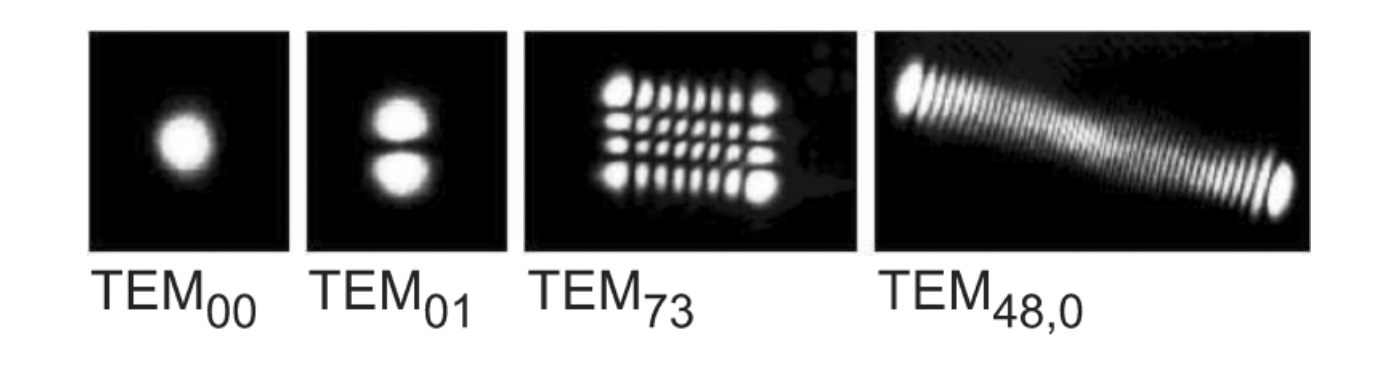
\includegraphics[width=0.9\linewidth]{figures/fabry-perot/gauss-modes-higher-order}
	\caption[Gaussian modes higher order of a simple Ti-sapphire laser]{Gaussian modes higher order of a simple Ti-sapphire laser.
		The asymmetry of the high modes are caused by technical inaccuracies of the resonator elements (mirrors, laser crystal).}
	\label{fig:gauss-modes-higher-order}
\end{figure}



\section{Fundamentals of Fabry-Pérot interferometers}


\subsection{Resonator losses}
For the following discussion of the \ac{FPI}, a two-mirror-resonator with the reflecting surfaces facing each other and air as medium in between is assumed.
The theoretical foundation is provided by the work of \textcite{ismail_fabry-perot_2016}.

The time the light needs for one roundtrip is given by
\begin{equation}
t_{RT} = \frac{2l}{c}
\end{equation}
where $l$ is the geometrical length of the resonator and $c$ is the speed of light in air.

The photon-decay time $\tau_c$ of the interferometer is then given by
\begin{equation}
\frac{1}{\tau_c} = - \frac{\ln(R_1 \cdot R_2)}{t_{RT}}
\end{equation}
where $R_1$ and $R_2$ are the corresponding intensity reflectivities of the mirrors.

The number of photons at frequency $\nu$ inside the resonator is described by the differential rate equation
\begin{equation}
\frac{d}{dt} \varphi(t) = - \frac{1}{\tau_c}\varphi(t).
\end{equation}
With a number $\varphi_s$ of photons at $t=0$ the integration gives
\begin{equation}
\label{eq:photon-decay}
\varphi(t)=\varphi_s e^{-t/\tau_c}
\end{equation}

\subsection{Resonance frequencies, free spectral range and spectral line shapes}
The round-trip phase shift at frequency $\nu$ is given by
\begin{equation}
\label{eq:round-trip-phase-shift-phi}
2 \phi(\nu) = 2 \pi \nu t_{RT} = 2 \pi \nu \frac{2l}{c}
\end{equation}
where $\phi(\nu)$ is the single-pass phase shift between the mirrors.

Resonances are visible for frequencies $\nu$ at which the light interferes constructively after one round trip.
Two adjacent resonance frequencies differ in their round trip phase shift by $2 \pi$.
Hence, the free spectral range $\Delta \nu_{FSR}$, the frequency difference between two adjacent resonance frequencies, can be calculated from equation~\eqref{eq:round-trip-phase-shift-phi}
\begin{align}
2\Delta\phi_{FSR} = 2\pi \\
\Rightarrow 2\pi\Delta\nu_{FSR}\frac{2l}{c} = 2\pi\\
\label{eq:free-spectral-range}
\Rightarrow \Delta\nu_{FSR} = \frac{c}{2l}
\end{align}

According to equation~\eqref{eq:photon-decay} the number of photons decays with the photon-decay time $\tau_c$.
With $E_{q,s}$ representing the initial amplitude, the electric field at $\nu_q$ is given by
\begin{equation}
E_q(t) =
\begin{cases}
E_{q,s} \cdot e^{i2\pi\nu_qt} \cdot e^{-t/(2\tau_c)} &  t \geq 0 \\
0 &  t < 0
\end{cases}
.
\end{equation}
The Fourier transformation of the electric field can be expressed as
\begin{equation}
\tilde{E}_q(\nu) = \int_{-\infty}^\infty E_q(t)e^{-i2\pi\nu t}dt = E_q(t) \int_{0}^\infty e^{.[1/(2\tau_c)+i2\pi(\nu-\nu_q)]t}dt = E_{q,s} \frac{1}{(2\tau_c)^{-1}+i2\pi(\nu-\nu_q)}.
\end{equation}
The normalized spectral line shape per unit frequency is then given by
\begin{align}
\label{eq:round-trip-phase-shift}
\tilde{\gamma_q}(\nu)&=\frac{1}{\tau_c}\left|\frac{\tilde{E}_q(\nu)}{E_{q,s}}\right|^2=\frac{1}{\tau_c}\left|\frac{1}{(2\tau_c)^{-1}+i2\pi(\nu-\nu_q)}\right|^2 = \frac{1}{\tau_c}\frac{1}{(2\tau_c)^{-2}+4\pi^2(\nu-\nu_q)^2} \\
&=\frac{1}{\pi}\frac{1/(4\pi\tau_c)}{1/(4\pi\tau_c)^2+(\nu-\nu_q)^2}
\end{align}
with $\int \tilde{\gamma_q}(\nu)d\nu=1$.

By defining the full-width-at-half-maximum linewidth (FWHM) $\Delta\nu_c$, $\tilde{\gamma_q}(\nu)$ can be obtained
\begin{equation}
\Delta \nu_c = \frac{1}{2\pi\tau_c} \Rightarrow \tilde{\gamma_q}(\nu) = \frac{1}{\pi}\frac{\Delta \nu_c/2}{\left(\Delta\nu_c/2\right)^2+\left(\nu-\nu_q\right)^2}.
\end{equation}
Afterwards the Cauchy lines are normalized so that the peak is at unity
\begin{equation}
\label{eq:cauchy}
\gamma_{q,L}(\nu)=\frac{\pi}{2}\Delta\nu_c\tilde{\gamma_q}(\nu)=\frac{(\Delta\nu_c)^2}{\left(\Delta \nu_c\right)^2+4\left(\nu-\nu_q\right)^2}
\end{equation}
with $\gamma_{q,L}(\nu_q)=1$.
\subsection{Airy distribution of Fabry-Pérot interferometers}

\begin{figure}[h]
	\centering
	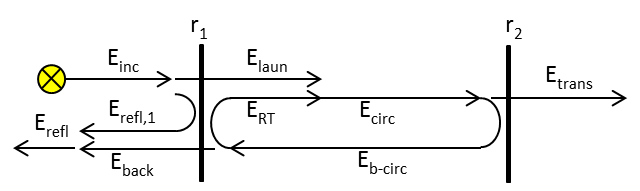
\includegraphics[width=0.7\linewidth]{figures/fabry-perot/Schematic_of_the_Fabry-Perot_interferometer}
	\caption[Fabry Pérot interferometer with electric field mirror reflectivities $r_1$ and $r_2$]{\ac{FPI} with electric field mirror reflectivities $r_1$ and $r_2$.
		Indicated in this figure are the electric fields resulting from an incoming $E_{inc}$, the reflected field $E_{refl,1}$ and transmitted field $E_{laun}$.
		$E_{circ}$ and $E_{circ,b}$ circulate inside the resonator, resulting in $E_{RT}$ after one round-trip. $E_{back}$ is the backwards transmitted field.\cite{noauthor_fabryperot_nodate}}
	\label{fig:schematicofthefabry-perotinterferometer}
\end{figure}
The response of the \ac{FPI} is calculated with the circulating-field approach~\cite{ismail_fabry-perot_2016}, where a steady-state is assumed.
$E_{circ}$ is the result of $E_{laun}$ interfering with $E_{RT}$.
$E_{laun}$ is the transmission of the incoming light $E_{inc}$ and $E_{RT}$ is $E_{circ}$ after one round-trip in the resonator, i.e., after the outcoupling losses of mirror 1 and 2.
Therefore, the field $E_{circ}$ can be calculated from $E_{launch}$ by
\begin{equation}
E_{circ} = E_{laun} + E_{RT} = E_{laun} + r_1 r_2 e^{-i 2 \phi} E_{circ} \Rightarrow \frac{E_{circ}}{E_{laun}} = \frac{1}{1 - r_1 r_2 e^{-i 2 \phi}}
\end{equation}
where $r_1$ and $r_2$ are the electric-field reflectivities of mirror 1 and 2.

The generic Cauchy distribution only considers light inside the mirrors and is defined as
\begin{equation}
A_{circ} = \frac{I_{circ}}{I_{laun}} = \frac{|E_{circ}|^2}{|E_{laun}|^2} = \frac{1}{\left|1 - r_1 r_2 e^{-i2\phi}\right|^2} = \frac{1}{\left(1-\sqrt{R_1 R_2}\right)^2 + 4\sqrt{R_1 R_2} \sin^2(\phi)}
\end{equation}
by using
\begin{align*}
\left|1-r_1 r_2 e^{-i2\phi}\right|^2 &= \left|1- r_1 r_2 \cos(2\phi) + i r_1 r_2 \sin(2\phi)\right|^2 = \left[1-r_1 r_2 \cos(2\phi)\right]^2 + r_1^2 r_2^2 \sin^2(2\phi) \\
 &=1+R_1 R_2 - 2\sqrt{R_1 R_2} \cos(2\phi) = \left(1-\sqrt{R_1 R_2}\right)^2 + 4 \sqrt{R_1 R_2} \sin^2(\phi)
\end{align*}
and additionally $R_i = r_i^2$ and $\cos(2\phi) = 1 -2\sin^2(\phi)$.

Commonly, light is sent through the \ac{FPI}. Therefore the following sections will use the Airy distribution $A'_{trans}$ described by
\begin{equation}
\label{eq:A-trans}
A'_{trans} = \frac{I_{trans}}{I_{inc}} = \frac{I_{circ} \cdot (1 - R_2)}{I_{laun} / (1 - R_1)} = (1-R_1)(1-R_2)A_{circ} = \frac{(1-R_1)(1-R_2)}{\left(1-\sqrt{R_1R_2}\right)^2+4\sqrt{R_1R_2}\sin^2(\phi)}
\end{equation}
with $\phi=\frac{\pi\nu}{\Delta \nu_{FSR}}$.

$A'_{trans}$ is displayed in figure~\ref{fig:airydistributionofafabry-perotinterferometer} for $R_1=R_2$. The peak value at one of its resonance frequencies calculates as follows
\begin{equation}
\max(A'_{trans}) = \frac{(1-R_1)(1-R_2)}{\left(1-\sqrt{R_1R_2}\right)^2} \stackrel{R_1=R_2}{=} 1.
\end{equation}

\begin{figure}[h]
	\centering
	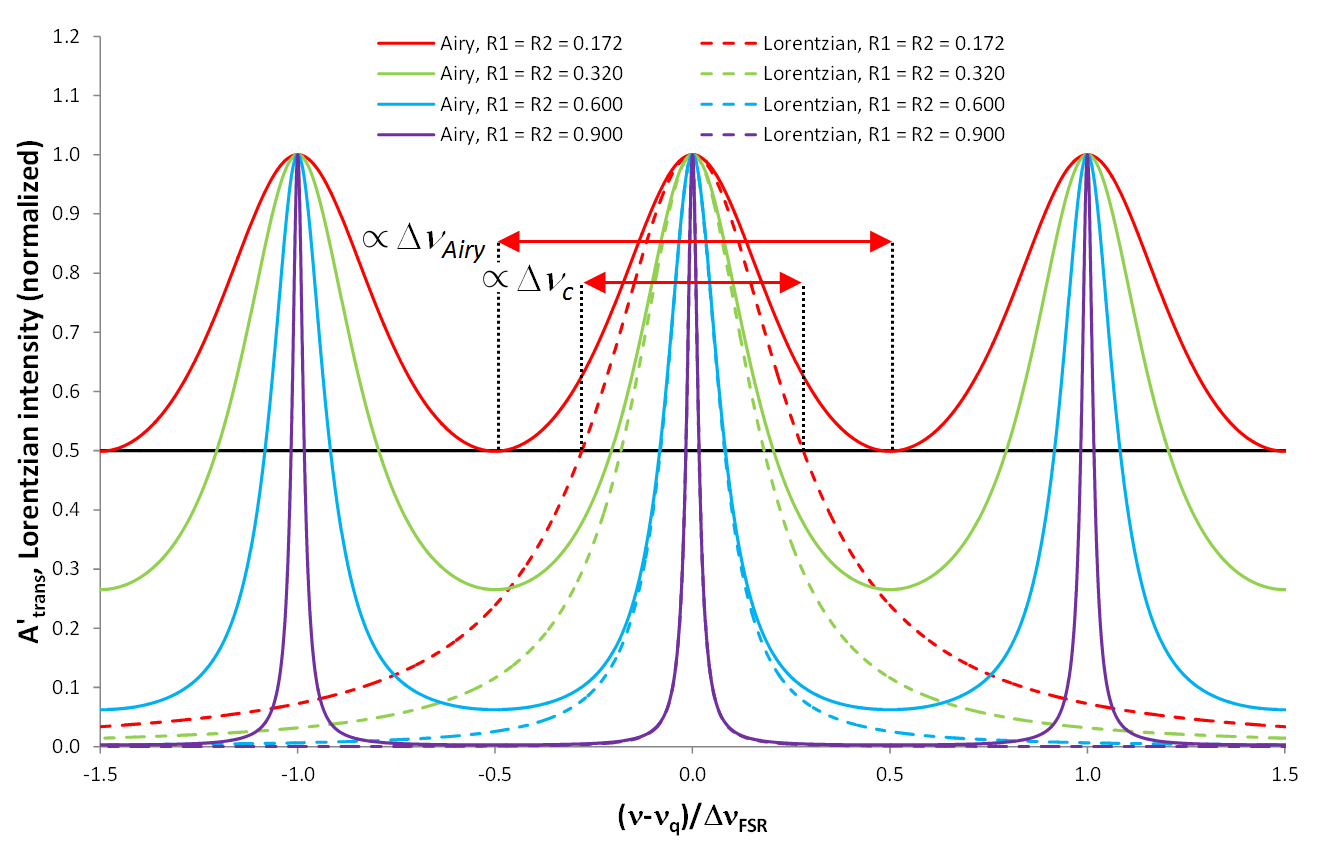
\includegraphics[width=0.8\linewidth]{figures/fabry-perot/Airy_distribution_of_a_Fabry-Perot_interferometer}
	\caption[Airy distribution $A'_{trans}$]{Airy distribution $A'_{trans}$ as described in equation~\eqref{eq:A-trans} compared to the Cauchy lines  $\gamma_{q,L}$ as described in equation~\eqref{eq:cauchy}~\cite{noauthor_fabryperot_nodate}.}
	\label{fig:airydistributionofafabry-perotinterferometer}
\end{figure}


\subsection{Airy linewidth and finesse}
The airy linewidth is defined as the \ac{FWHM} of $A'_{trans}$. It can be set in relation with the free spectral range $\Delta \nu_{FSR}$ and the mirror reflectivities as follows.

$A'_{trans}$ decreases to half of its peak value at $A'_{trans}(v_q) / 2$ when the phase shift $\phi$ changes by the amount $\Delta\phi$ so that the denominator of $A'_{trans}$ in equation~\eqref{eq:A-trans}  is twice as big
\begin{align}
\left(1-\sqrt{R_1R_2}\right)^2=4\sqrt{R_1R_2}\sin^2(\Delta\phi) \\
\label{eq:phase-shift-R}
\Rightarrow \Delta\phi=\arcsin\left(\frac{1-\sqrt{R_1R_2}}{2\sqrt[4]{R_1R_2}}\right)
\end{align}
With equation~\eqref{eq:round-trip-phase-shift-phi} and \eqref{eq:free-spectral-range}, the phase shift can be expressed as
\begin{align}
\phi &= \frac{\pi \nu}{\Delta \nu_{FSR}} \\
\label{eq:phase-shift-nu}
\Rightarrow \Delta \phi &= \frac{\pi (\Delta \nu_{Airy}/2)}{\Delta \nu_{FSR}}.
\end{align}
Therefore, with equation~\eqref{eq:phase-shift-R} and \eqref{eq:phase-shift-nu} the \ac{FWHM} linewidth is given by
\begin{equation}
\Delta \nu_{Airy} = \Delta \nu_{FSR}\frac{2}{\pi}\arcsin\left(\frac{1-\sqrt{R_1R_2}}{2\sqrt[4]{R_1R_2}}\right).
\end{equation}

The finesse of the Airy distribution of a \ac{FPI} is defined as
\begin{equation}
\label{eq:f-airy}
F_{Airy} := \frac{\Delta \nu_{FSR}}{\Delta \nu_{Airy}} = \frac{\pi}{2}\left[\arcsin\left(\frac{1-\sqrt{R_1R_2}}{2\sqrt[4]{R_1R_2}}\right)\right]^{-1}
\end{equation}
and is therefore only dependent on the mirror reflectivities $R_1$ and $R_2$.

\begin{figure}[H]
	\centering
	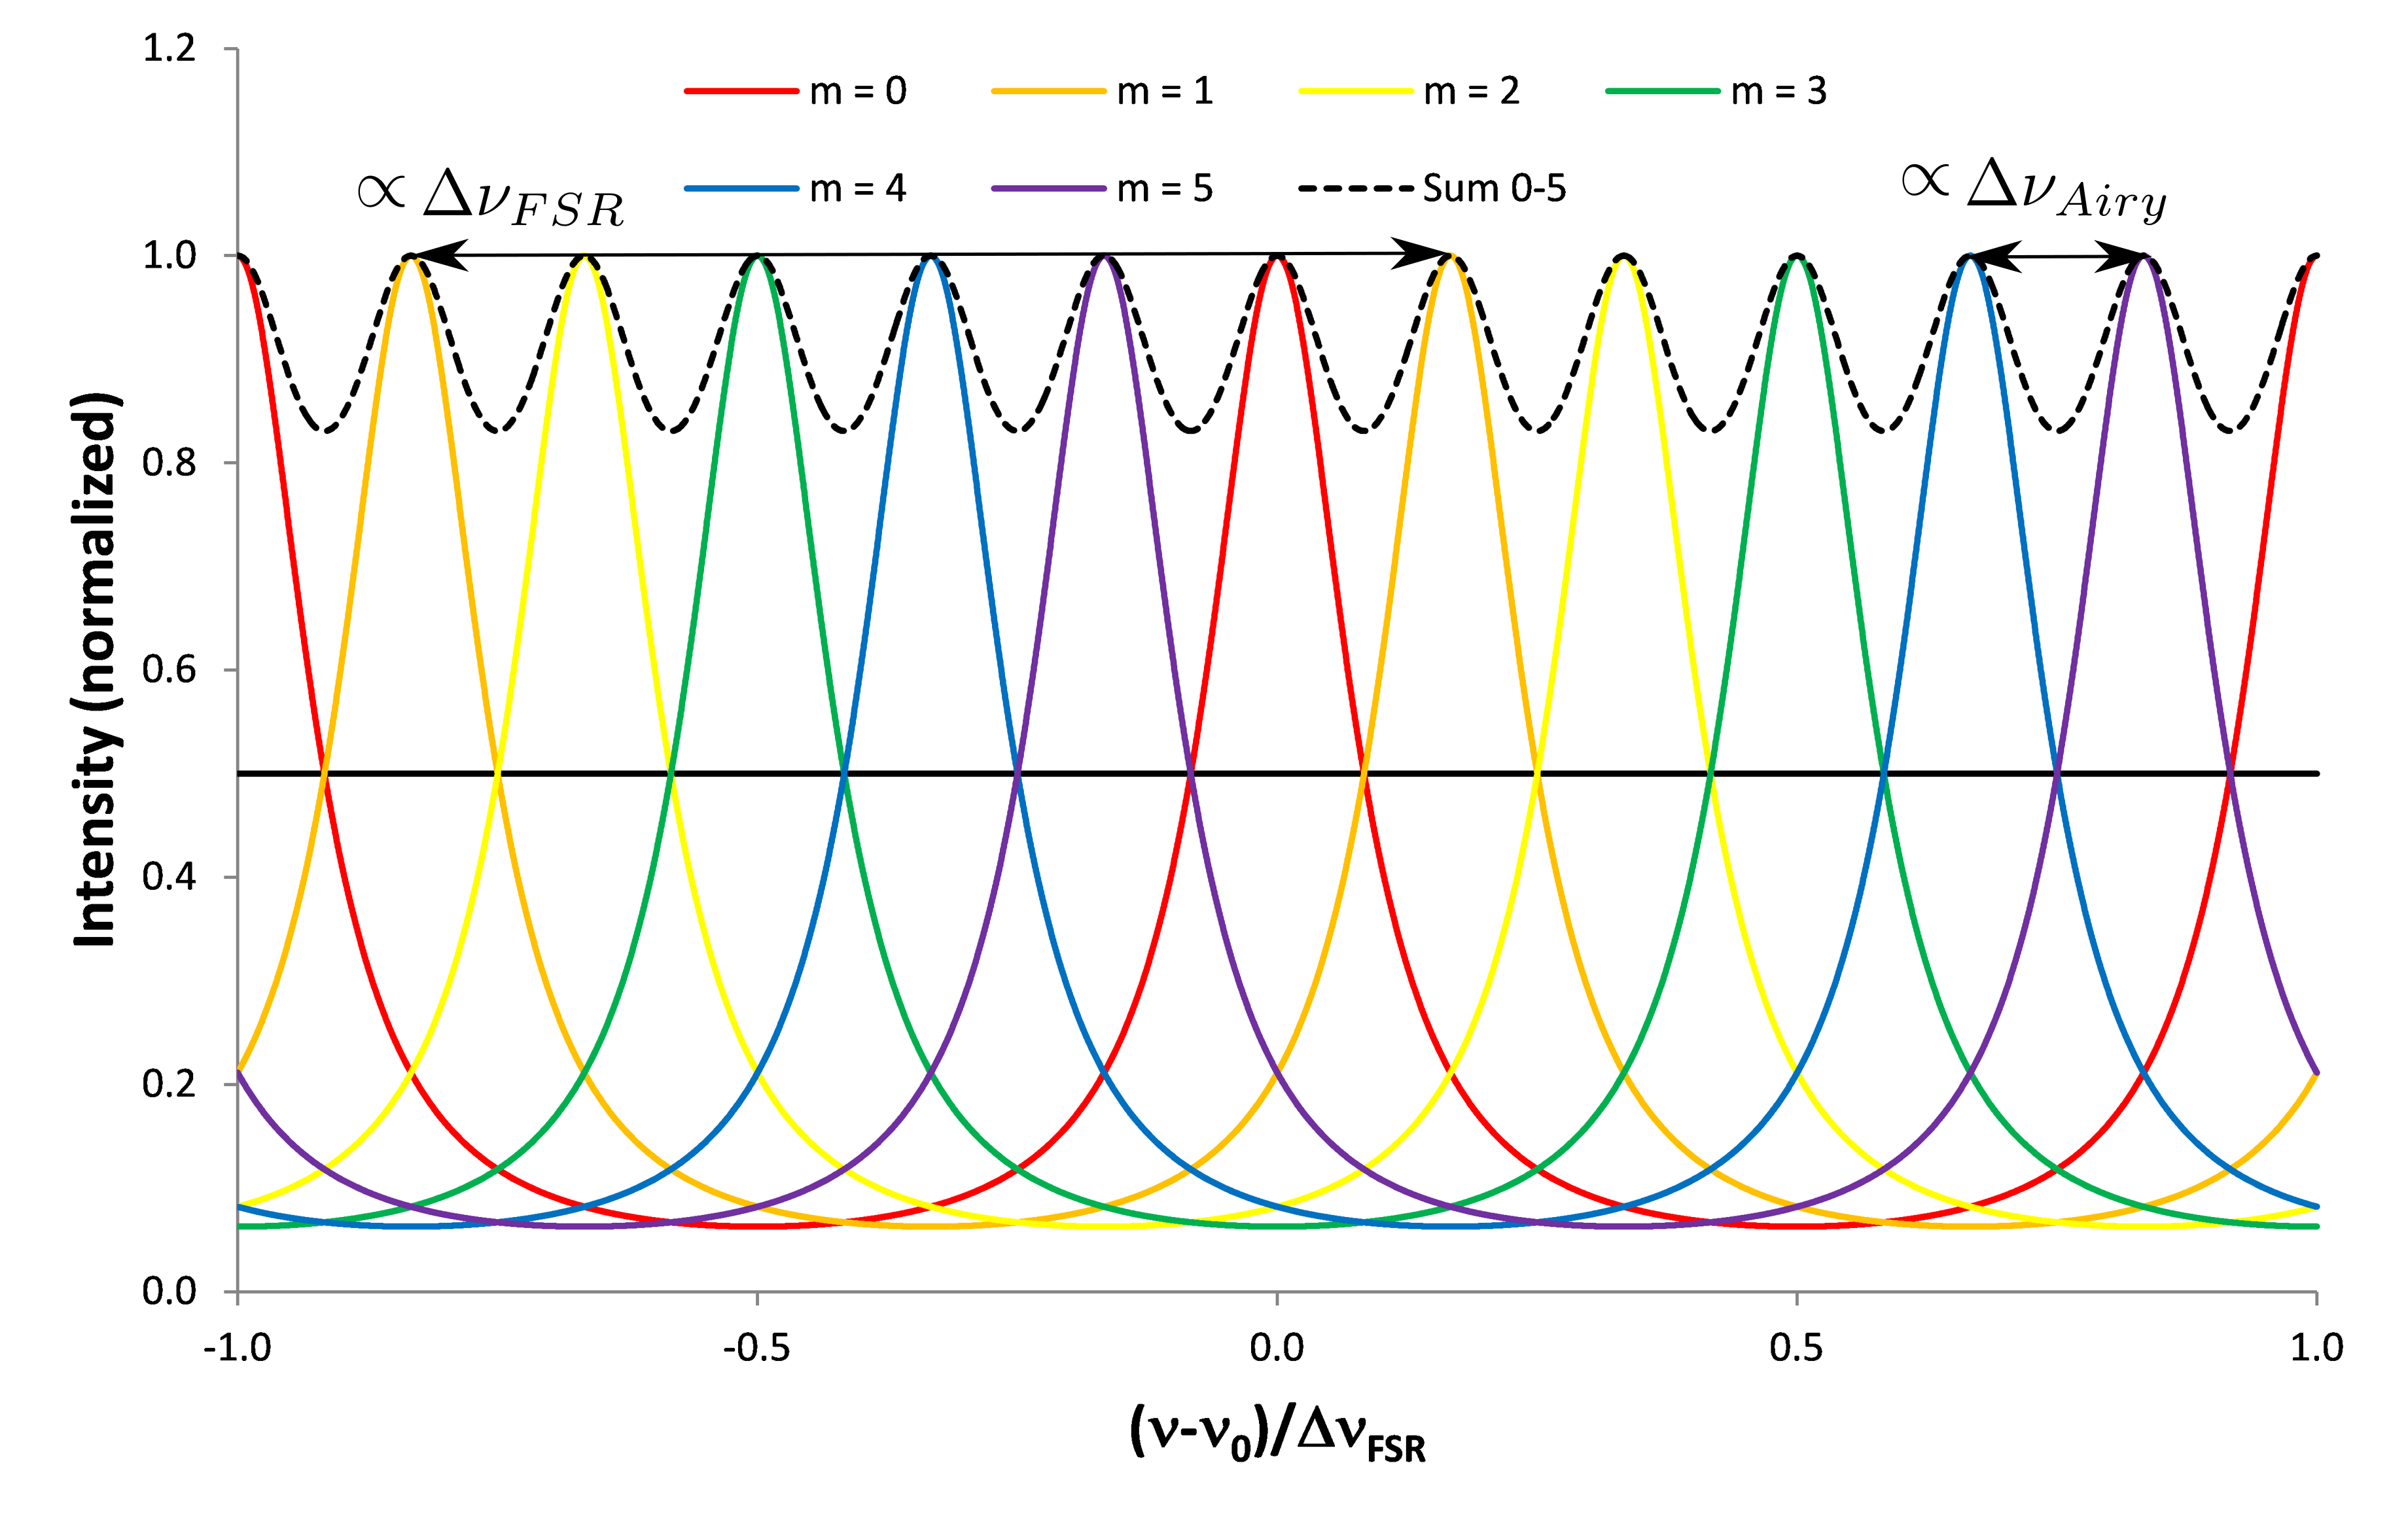
\includegraphics[width=0.8\linewidth]{figures/fabry-perot/Airy_finesse_of_a_Fabry-Perot_interferometer}
	\caption[Demonstration of the physical meaning of the Airy finesse $F_{Airy}$]{Demonstration of the physical meaning of the Airy finesse $F_{Airy}$.
		The coloured lines are Airy distributions created by light at distinct frequencies $\nu_m$, while scanning the resonator length. When the light occurs at frequencies $\nu_m = \nu_q+m\Delta \nu_{Airy}$, the adjacent Airy distributions are separated from each other by $\nu_{Airy}$, therefore fulfilling the Taylor criterion.
		Since in this example $F_{airy}=6$  exactly six peaks fit inside the free spectral range.
		As can be seen in the figure the Airy finesse $F_{Airy}$ quantifies the maximum number of peaks that can be resolved ~\cite{noauthor_fabryperot_nodate}.}
	\label{fig:airyfinesseofafabry-perotinterferometer}
\end{figure}


The Airy finesse is the determining property when it comes to the spectral resolution of the \ac{FPI}. This can be made visible by comparing its message with the Taylor criterion for the resolution of two adjacent peaks.
The Taylor criterion proposes that two spectral lines are resolvable when the separation of the maxima is greater than the \ac{FWHM}.
As displayed in figure~\ref{fig:airyfinesseofafabry-perotinterferometer}, the Airy finesse is equal to the number of Airy distributions originating from light at certain frequencies $\nu_m$ which do not overlap at a point higher than half of their maxima.
Hence, the Airy finesse describes the spectral resolution in a way that is consistent with the Taylor criterion.



\subsection{Mode matching and spatial filtering}
\label{subsec:mode-matching-spatial-filtering}
One fundamental challenge of Fabry Pérot interferometry is how to efficiently couple an incident beam of light into a given mode of the resonator.
The following discussion is based on the work of \textcite{yariv_photonics:_2007} and \textcite{meschede_optik_2008}.
\begin{figure}[H]
	\centering
	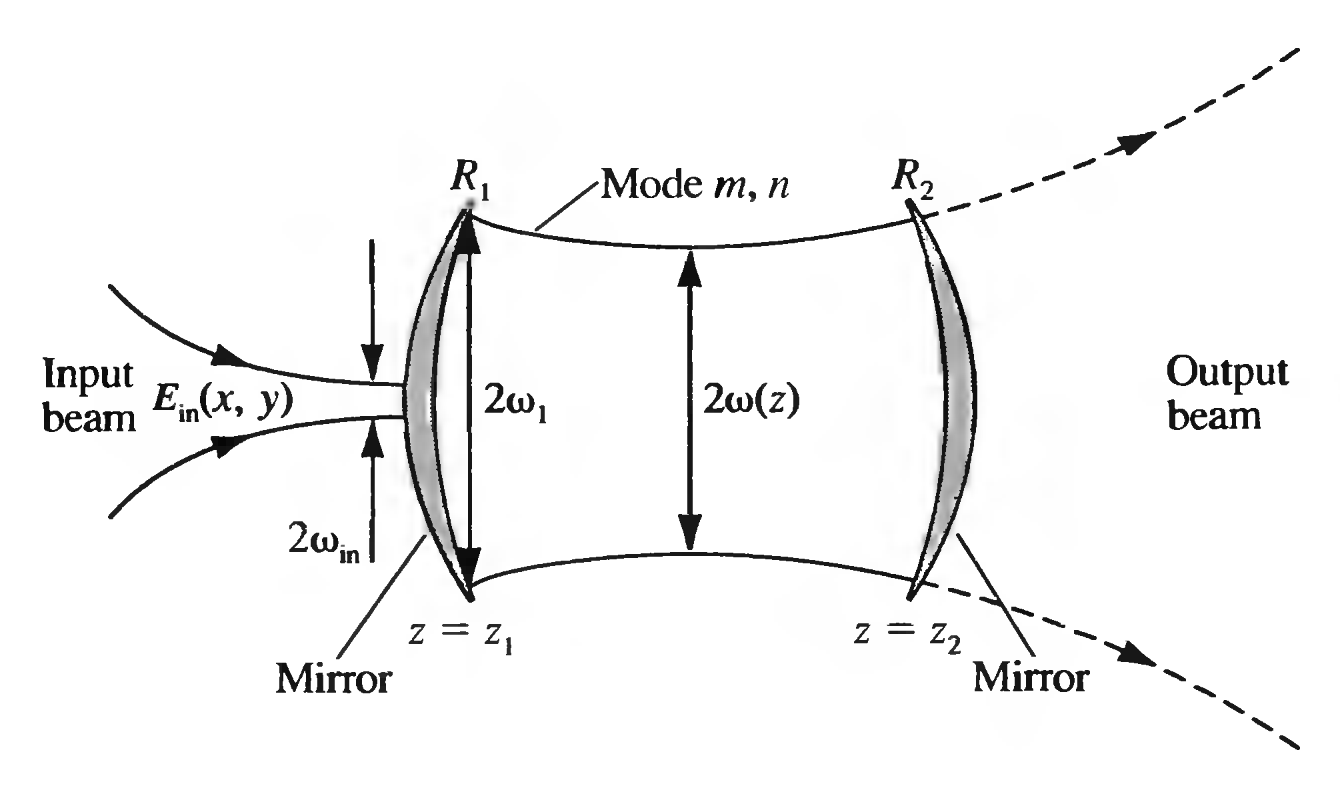
\includegraphics[width=0.7\linewidth]{figures/fabry-perot/excitation-of-transverse-mode}
	\caption{Incident monochromatic beam of light exciting transverse mode $m$, $n$ of a resonator~\cite{yariv_photonics:_2007}}
	\label{fig:excitation-of-transverse-mode}
\end{figure}

In sketched with figure~\ref{fig:excitation-of-transverse-mode}, an input beam $E_{in}$ propagates into the resonator and potentially excite its modes $E_{mn}(x,y)$, where $m$, $n$ are the transverse mode integers of the Gaussian beam of the optical resonator.
Since $E_{mn}(x,y)$ describes a complete orthogonal set of wavefunctions they satisfy
\begin{equation}
\label{eq:complete-set-mn-modes}
\iint E_{mn}(x,y) E^*_{m'n'}(x,y) dx dy = 0 \quad \mathrm{unless} \ m=m' \ \mathrm{and} \ n=n'.
\end{equation}
and
\begin{equation}
\label{eq:superposition-mn-modes}
E_{in}(x,y) = \sum_{mn}a_{mn}E_{mn}(x,y)
\end{equation}
where $a_{mn}$ are constants.
By multiplying both sides of equation~\eqref{eq:superposition-mn-modes} with $E_{mn}^*$, integrating over the whole $x$-$y$-plane and using equation~\eqref{eq:complete-set-mn-modes}, the following expression can be obtained
\begin{equation}
\label{eq:a-mn}
a_{mn}=\frac{\iint E_{in}(x,y)E^*_{mn}(x,y) dx dy}{\iint E_{mn}(x,y)E^*_{mn}(x,y) dx dy}
\end{equation}
The efficiency of coupling an incident field into a spatial mode $E_{mn}$ is defined as
\begin{equation}
\label{eq:coupling-efficiency-first}
\eta_{mn}=\frac{\textrm{Power coupled into mode } mn}{\textrm{Total incident power}}=
\frac{\iint \left|a_{mn} E_{mn}(x,y)\right|^2 dx dy}{\iint \left|E_{in}(x,y)\right|^2 dx dy}.
\end{equation}
By inserting equation~\eqref{eq:a-mn} into equation~\eqref{eq:coupling-efficiency-first} the following expression can be obtained
\begin{equation}
\label{eq:coupling-efficiency-second}
\eta_{mn}= \frac{\left|\iint E_{in}(x,y)E^*_{mn}(x,y) dx dy\right|^2}{\iint \left|E_{in}(x,y)\right|^2 dx dy \cdot \iint \left|E_{mn}(x,y)\right|^2 dx dy}.
\end{equation}
From equation~\eqref{eq:coupling-efficiency-second} can be deduced that for an input beam with the \textit{same} spatial dependency as the mode to be excited
\begin{equation}
E_{in}(x,y) \sim E_{mn}(x,y)
\end{equation}
all of the incident power goes into $E_{mn}$, i.e. $\eta_{mn}=1$ and all other $\eta_{m'n'}$ are zero.
Usually, the fundamental TEM$_{00}$ mode is desired and equation~\eqref{eq:coupling-efficiency-second} implies that a pure Gaussian beam excites only the fundamental mode and the interferometer will then irradiate a pure Gaussian beam as well.
In practise, additional measures are necessary such as matching the radius of curvature by Gaussian beam focusing.

\begin{figure}[h]
	\centering
	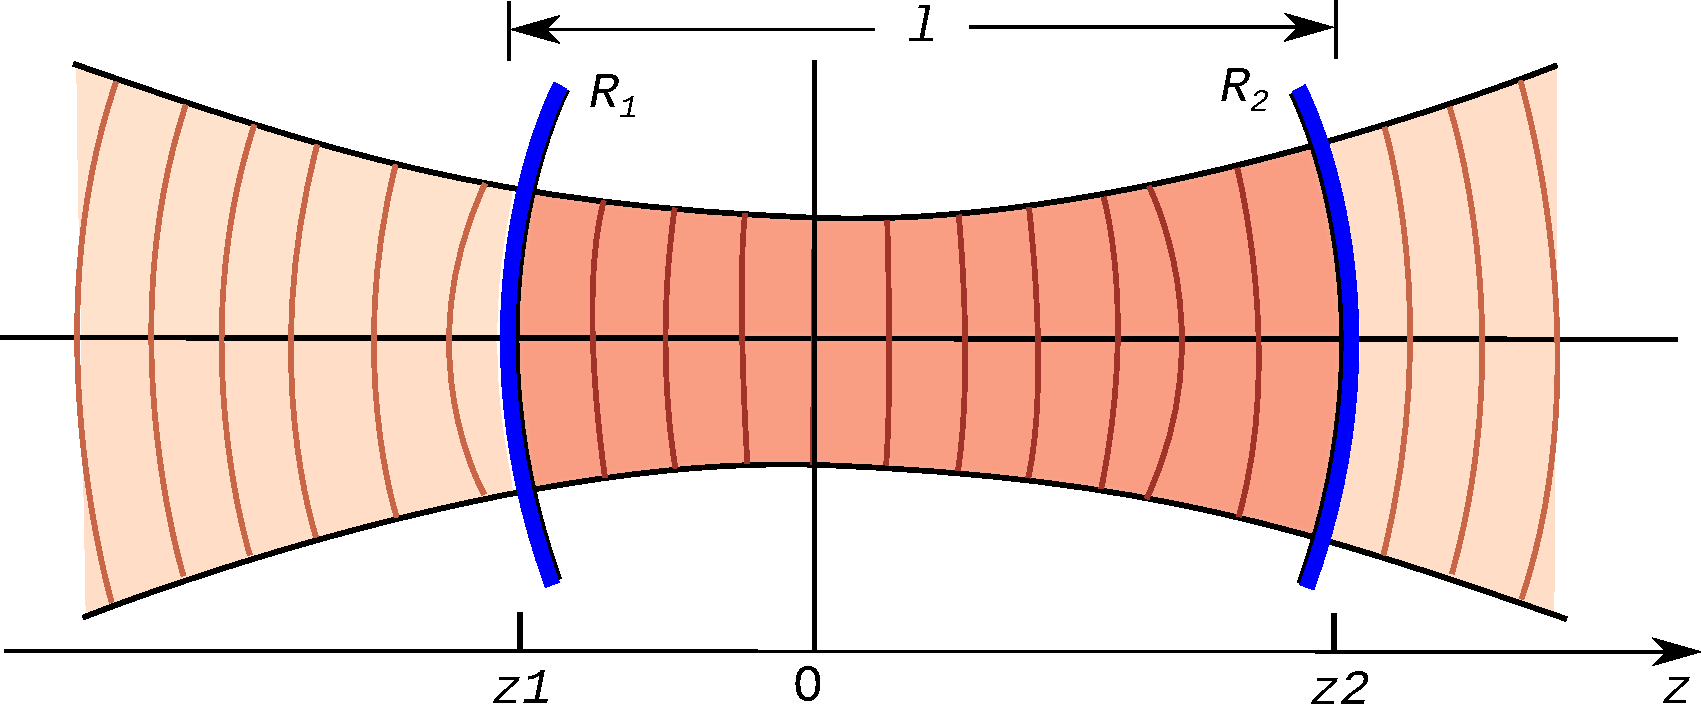
\includegraphics[width=0.8\linewidth]{figures/fabry-perot/gaussian-beam-focusing}
	\caption[Mode matching of an Gaussian beam into a Fabry Pérot interferometer.]
	{Mode matching of an Gaussian beam into a Fabry Pérot interferometer.
		Incoming Gaussian beam described by $q_{in}$ transformed by a lens into a Gaussian beam described by $q_{out}$.
		The parameters $b_1$ and $b_2$ describe the radii of the two mirrors.}
	\label{fig:gaussian-beam-focusing}
\end{figure}

In order to match the radius of curvature of the incoming Gaussian beam with the radius of curvature of the resonator a lens is inserted as depicted in figure~\ref{fig:gaussian-beam-focusing}. Light with a beam waist of $\omega_{01}$ gets focused into the resonator. Transformations by thin lenses can be described with the ray transfer matrix introduced in subsection~\ref{subsec:gaussian-beam}:
\begin{equation}
\begin{pmatrix}
A & B \\
C & D
\end{pmatrix}
=
\begin{pmatrix}
1 & 0 \\
\frac{-1}{f} & 1
\end{pmatrix}
\end{equation}
with $f$ as the wavelength of the lens.
The incoming beam described by $q_{in}$ is transformed by the lens into a beam described by $q_{out}$ according to equation~\eqref{eq:beam-waist} and \eqref{eq:ABCD-rule}
\begin{equation}
q_{in} = z + i \frac{\pi n \omega_{0,in}^2}{\lambda} \qquad \mathrm{and} \qquad
q_{out} = \frac{q_{in}}{q_{in} \cdot \frac{-1}{f} + 1} =  z + i \frac{\pi n \omega_{0,out}^2}{\lambda}
\end{equation}
with $n\approx 1$ for air. Together with equation~\eqref{eq:beam-waist} to following relation can be deduced
\begin{equation}
\label{eq:w-o-out}
\omega_{0,out}^2 = \frac{\omega_{0,in}^2}{\left(1-\frac{z}{f}\right)^2+\left(\frac{\pi \omega_{0,in}}{\lambda f}\right)^2}.
\end{equation}
The radii of curvature have to match.
For given mirrors (described by $R_{mirror}$) and lens (described by $f$) the input beam waist has to be adjusted according to equation~\eqref{eq:radius-wavefronts} and \eqref{eq:beam-waist}
\begin{align}
R_{mirror} \stackrel{!}{=} R_{gauss}(z= l/2)\\
R_{mirror} \stackrel{!}{=} \frac{l}{2} \left(1+\left(\frac{2z_{0,out}}{l}\right)^2\right) \\
\label{eq:R-mirror-1}
R_{mirror} \stackrel{!}{=} \frac{l}{2} \left(1+\left(\frac{2\omega_{0,out}^2 \pi}{l \lambda}\right)^2\right).
\end{align}
Inserting equation~\eqref{eq:R-mirror-1} into equation~\eqref{eq:w-o-out} results in the condition for mode matching
\begin{equation}
\label{eq:R-mirror-2}
R_{mirror} = \frac{l}{2} \left(1+\left(\frac{2 \omega_{0,in}^2 \pi}{\left(\left(1-\frac{z}{f}\right)^2+\left(\frac{\pi \omega_{0,in}}{\lambda f}\right)^2\right)l \lambda}\right)^2\right).
\end{equation}

One way to further suppress higher modes is \textit{spatial filtering}. It can be seen in figure~\ref{fig:gauss-modes-higher-order} that the effective area of a mode increases with its order $(m, n)$. Figure~\ref{fig:spatial-filtering-of-gauss-modes} shows one way to suppress higher modes consisting of a focusing lens and a pin hole which diameter matches the one of the TEM$_{00}$ mode.

\begin{figure}[H]
	\centering
	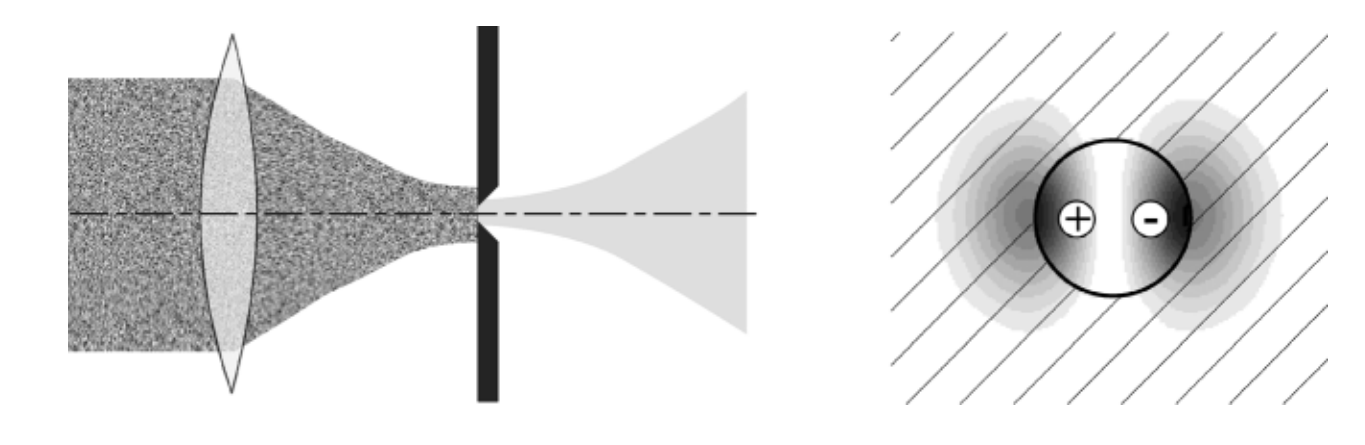
\includegraphics[width=0.8\linewidth]{figures/fabry-perot/spatial-filtering-of-gauss-modes}
	\caption[Spatial filtering of Gauss modes.]{Spatial filtering of Gauss modes.
		In front of the aperture, the beam consists of a superposition of multiple Gauss modes.
		In the example of TEM$_{01}$ is displayed how higher modes are suppressed by the aperture.~\cite{meschede_optik_2008}}
		\label{fig:spatial-filtering-of-gauss-modes}
	\end{figure}



\subsection{Confocal setup}
\label{subsec:confocal-setup}

If the incoming beam would represent a perfect TEM$_{00}$ mode, spatial filtering would not be necessary and mode matching would not have to be done as precise.
Unfortunately, this can not always be guaranteed and counteractions like mode matching and spatial filtering discussed in subsection~\ref{subsec:mode-matching-spatial-filtering} are tedious and error prone.
Arranging the mirrors of an \ac{FPI} into a confocal arrangement reduces the need for these measures.
By giving up the ability to choose different free spectral ranges with a given pair of mirrors, the confocal setup liberates from mode matching considerations as the cavity is mode degenerated, i.e. the frequency of certain axial and transverse cavity modes are the same.
The following discussion is based on the work of \textcite{hercher_spherical_1968}.

A quasi-monochromatic beam of wavelength $\lambda_0$ is composed of transverse modes TEM$_{\textrm{mnq}}$, where the subscripts $m$ and $n$ denote the amplitude distribution of the normal mode on a surface of constant phase and $q$ the number of axial modes inside the resonator.
Each of these modes resonates for mirror separations satisfying
\begin{equation}
l = \frac{\lambda_0}{2}\{q + \left(1 + m + n\right) \cos^{-1}\left[(1-l/b_1)(1-l/b_2)\right]^{1/2}\}
\end{equation}
where the parameters $b_1$ and $b_2$ describe the radii of the two mirrors as can be seen in figure~\ref{fig:gaussian-beam-focusing}.

For the confocal setup $l=b_1=b_2$ justifies the approximation
\begin{equation}
l \approx \frac{\lambda_0}{2} \left[q + \left(1+m+n\right)\right].
\end{equation}
The modes resonate at mirror separations of either
\begin{align}
l = \frac{\lambda_0}{2}(p+1) \qquad p&\in\mathbb{N} \textrm{ and } (m+n) \textrm{ even,} \\
l = \frac{\lambda_0}{2}(p) \qquad p&\in\mathbb{N} \textrm{ and } (m+n) \textrm{ odd.}
\end{align}
If mode matching is not executed, it can be assumed that the incoming beam consists of an approximately equal number of even and odd transverse modes.
The resonance cavity length $l$ does not depend on $n$,$m$ and $q$ anymore but only on one integer $p$. The transversal modes are degenerate and fulfil
\begin{equation}
\label{eq:confocal-degenerate}
l = \frac{\lambda_0 p}{2}.
\end{equation}
It can be additionally concluded from equation~\eqref{eq:confocal-degenerate} that a change of $\lambda_0/2$ in the mirror separation scans through one free spectral range.
\section{Simulation}

The goal in building up a scanning \ac{FPI} is to resolve features of the emission spectra of GaAs \aclp{QD} described in chapter~\ref{chapter:quantum-dot}.
More precisely, it is intended to resolve the shape of the \ac{ZPL} and the \ac{PSB}.
Equation~\ref{eq:f-airy} shows that the finesse is constant for a given pair of mirrors.
If the spectrum to be resolved is broad, a higher free spectral range $\Delta \nu_{FSR}$ has to be chosen, under the loss of resolution.
If the spectrum contains fine details which need to be resolved, a lower $\nu_{Airy}$ has to be chosen, which results in a lower free spectral range $\Delta \nu_{FSR}$.
Hence, the thin \ac{ZPL} and the broad \ac{PSB} can not be resolved with the same setup.
Instead, the mirror distances have to be adjusted and in the confocal setup discussed in subsection~\ref{subsec:confocal-setup} the mirrors have to be changed as well.

The zero-phonon line is described with a Cauchy distribution
\begin{equation}
\Phi_{ZPL}(\lambda) = \frac{1}{\pi \cdot \Delta\lambda_{ZPL} \cdot 0.5 \left[1+\left(\frac{\lambda - \lambda_{0, ZPL}}{\Delta\lambda_{ZPL} \cdot 0.5}\right)^2\right]}
\end{equation}
with $\lambda_{0, zero}$ as the center wavelength and $\Delta\lambda_{ZPL}$ as the spectral range of the zero-phonon line which can be found in table~\ref{tab:quantum-dot-emission}.

The phonon side band is described with a Gauss distribution
\begin{equation}
\Phi_{PSB}(\lambda) = \frac{1}{\sqrt{2\cdot\pi\cdot \Delta\lambda_{PSB}^2}}\cdot exp\left(-\frac{(\lambda - \lambda_{0, PSB})^2}{2\cdot \Delta\lambda_{PSB}^2}\right)
\end{equation}
with $\lambda_{0, PSB}$ as the center wavelength and $\Delta\lambda_{PSB}$ as the spectral range of the phonon side band which can be found in table~\ref{tab:quantum-dot-emission} as well.

Together they describe the excitonic emission of the \ac{QD}
\begin{equation}
\Phi_{dot}(\lambda) = \Phi_{ZPL}(\lambda) + \Phi_{PSB}(\lambda)
\end{equation}
depicted in figure~\ref{fig:quantumdotemissionwavelengthenergy}.

\begin{figure}[H]
	\centering
	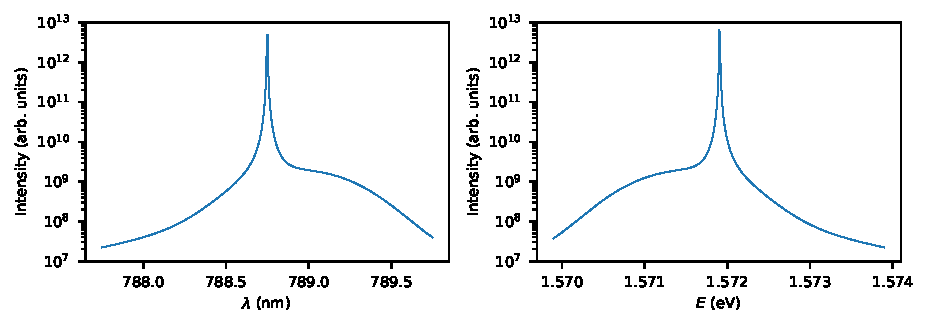
\includegraphics{figures/fabry-perot/plots/quantum_dot_emission_wavelength_energy}
	\caption[Simulated exciton emission of a GaAs quantum dot]{Simulated exciton emission of a GaAs quantum dot plotted dependant on (a) the wavelength $\lambda$ or (b) the energy $E$.
		The parameters can be found in table~\ref{tab:quantum-dot-emission}.}
	\label{fig:quantumdotemissionwavelengthenergy}
\end{figure}

$\Phi_{dot}(E)$ is transmitted through the \ac{FPI}.
As discussed the mirror distance $l$ is adjusted to a value which depends if a resolved \ac{ZPL} or a resolved \ac{PSB} is desired.
A comparison of the \ac{FPI} transmission $A'_{trans}(E)$ described in equation~\ref{eq:A-trans} with $R_1=R_2=\SI{98}{\percent}$ and $\Phi_{dot}(E)$ is shown in figure~\ref{fig:simulation-comparison-dot-fabry-perot-modes}.
\begin{figure}[H]
	\centering
	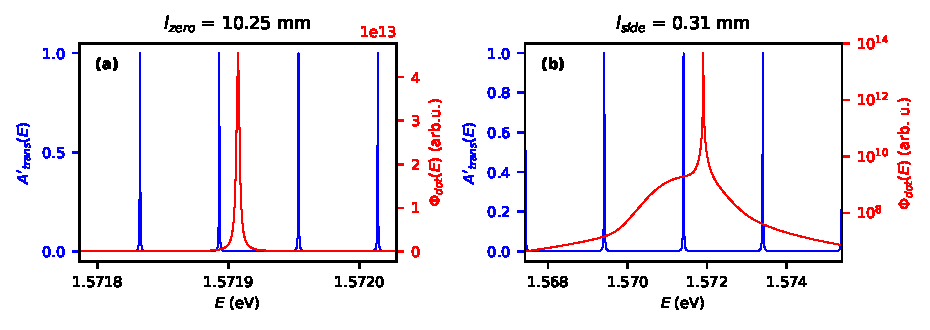
\includegraphics[width=\linewidth]{figures/fabry-perot/plots/simulation-comparison-dot-fabry-perot-modes}
	\caption{Transmission of the FPI modes $A'_{trans}$ compared to the exciton emission $\Phi_{dot}(E)$ for (a) ZPL and (b) PSB.}
	\label{fig:simulation-comparison-dot-fabry-perot-modes}
\end{figure}

The \ac{FPI} scans by continuously varying the mirror distance $l$ with a certain stepsize $\Delta l$ and measuring the output-photon-flux every time.
This process is sketched in figure~\ref{fig:simulation-comparison-dot-fabry-perot-sweep}.

\begin{figure}[H]
	\centering
	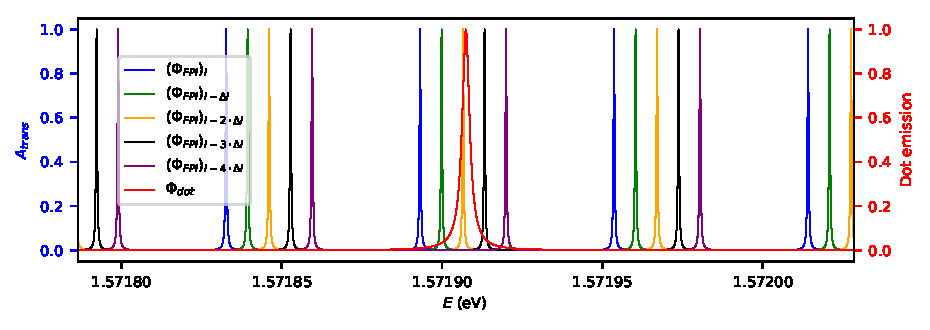
\includegraphics[width=\linewidth]{figures/fabry-perot/plots/simulation-comparison-dot-fabry-perot-sweep}
	\caption{Transmissions of the FPI modes $A'_{trans}$ (blue) for different mirror distances $l - m \cdot \Delta l$ with $m \in \mathbb{N}$ compared to the exciton emission $\Phi_{dot}(E)$ (red).}
	\label{fig:simulation-comparison-dot-fabry-perot-sweep}
\end{figure}


The unnormalized output-photon-flux of the scanning \ac{FPI} is then described with the convolution of $\Phi_{dot}(E)$ and $A'_{trans}(E)$
\begin{equation}
\tilde{\Phi}_{FPI}(E) = \int^{E_0 + n \cdot \Delta}_{E_0 - n  \cdot \Delta}  \Phi_{dot}(E')A'_{trans}(E - E') dE'
\end{equation}
with $E_0$ as the central energy of the exciton emission line, $\Delta$ as the free spectral range and $2n=4$ as the number of airy peaks considered for the numerical convolution.

\begin{figure}[H]
	\centering
	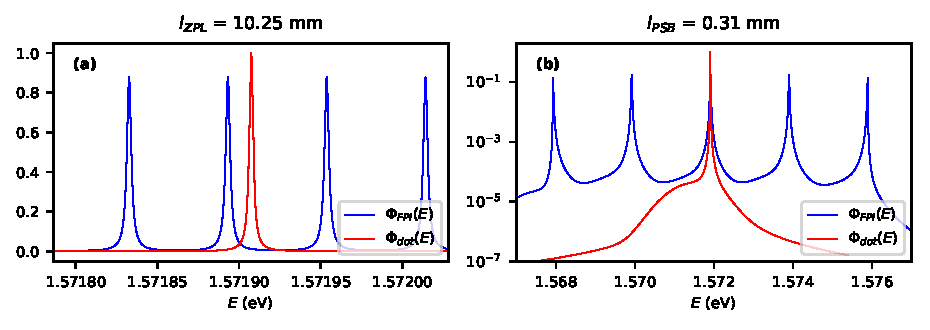
\includegraphics[width=\linewidth]{figures/fabry-perot/plots/simulation-comparison-dot-fabry-perot-output}
	\caption{Output-photon-flux of the scanning FPI $\Phi_{FPI}(E)$ (blue) compared to the exciton emission $\Phi_{dot}(E)$ (red) for (a) ZPl and (b) PSB.}
	\label{fig:simulation-comparison-dot-fabry-perot-output}
\end{figure}

$\tilde{\Phi}_{FPI}(E)$ can then be normalized with the integral of $A'_{trans}(E)$ over the same range
\begin{equation}
\Phi_{FPI}(E) =\frac{\tilde{\Phi}_{FPI}(E)}{\int^{E_0 + n \cdot \Delta}_{E_0 - n \cdot \Delta} A'_{trans}(E) dE}
\end{equation}
A comparison of $\Phi_{FPI}(E)$ and $\Phi_{dot}(E)$ is shown in figure~\ref{fig:simulation-comparison-dot-fabry-perot-output}.


From now on, only the \ac{ZPL}-path is shown as no new information is gained by examining both.
In order to estimate the accuracy of the scanning \ac{FPI}, the \ac{FPI} modes are shifted by $\Delta E$ in order to overlap with $\Phi_{dot}(E)$ as depicted in figure~\ref{fig:simulation-comparison-dot-fabry-perot-output-error}(a)
\begin{equation}
\overline{\Phi}_{FPI}(E) = \Phi_{FPI}(E - \Delta E).
\end{equation}
Afterwards, the absolute difference between those two $|\Phi_{dot}(E) - \Phi_{FPI}(E-\Delta E)|$ is calculated as shown in figure~\ref{fig:simulation-comparison-dot-fabry-perot-output-error}(b).
Now the relative error of  $\Phi_{fabry,perot}(E)$  for the given parameters and compared to the actual excitonic \ac{QD} emission  can be calculated
\begin{equation}
\epsilon = \frac{\int^{E_0 + \Delta / 2}_{E_0 - \Delta / 2} \left|\overline{\Phi}_{\text{FPI}}(E) - \Phi_{\text{dot}}(E)\right| dE }{\int^{E_0 + \Delta / 2}_{E_0 - \Delta / 2} \Phi_{\text{dot}}(E) dE}
\end{equation}
For the parameters in the \ac{ZPL} path this gives $\epsilon_{ZPL}=\SI{10.57}{\percent}$.


\begin{figure}[H]
	\centering
	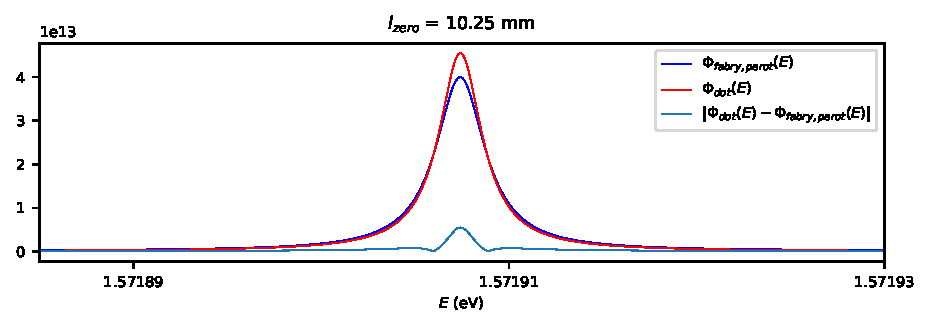
\includegraphics[width=\linewidth]{figures/fabry-perot/plots/simulation-comparison-dot-fabry-perot-output-error}
	\caption{In (a) the shifted output-photon-flux of the scanning FPI $\overline{\Phi}_{FPI}(E)$ (blue) compared to the exciton emission $\Phi_{dot}(E)$ (red) is displayed.
	In (b) the absolute difference between those two $ \left|\overline{\Phi}_{\text{FPI}}(E) - \Phi_{\text{dot}}(E)\right|$ (light blue) is additionally shown.}
	\label{fig:simulation-comparison-dot-fabry-perot-output-error}
\end{figure}


\newpage


\section{Setup and measurement}

Multiple \ac{FPI} setups were built up in order to test their suitability to resolve \ac{QD} emission.
The first version featured planar mirrors, while their distance was coarsely tunable with an adjustable platform and finely tunable with a piezoelectrical actuator.
However this setup with planar mirrors proved to be highly unstable and was therefore discarded.
The second version used smaller, planar-convex mirrors and a ground plate made of molybdenum.
This resulted in a stable \ac{FPI} which was also adjustable for various free-spectral ranges.
The measurements discussed in section~\ref{sec:fabry-measurements} are obtained with this setup.
However, the effort needed to mode-match for every measurement is too large to actually use it in further experiments.
That is why the confocal setup will be used in the future, even though the freedom to adjust the free-spectral range is lost.

\begin{figure}[H]
	\centering
	\begin{subfigure}[b]{0.48\textwidth}
		\centering
		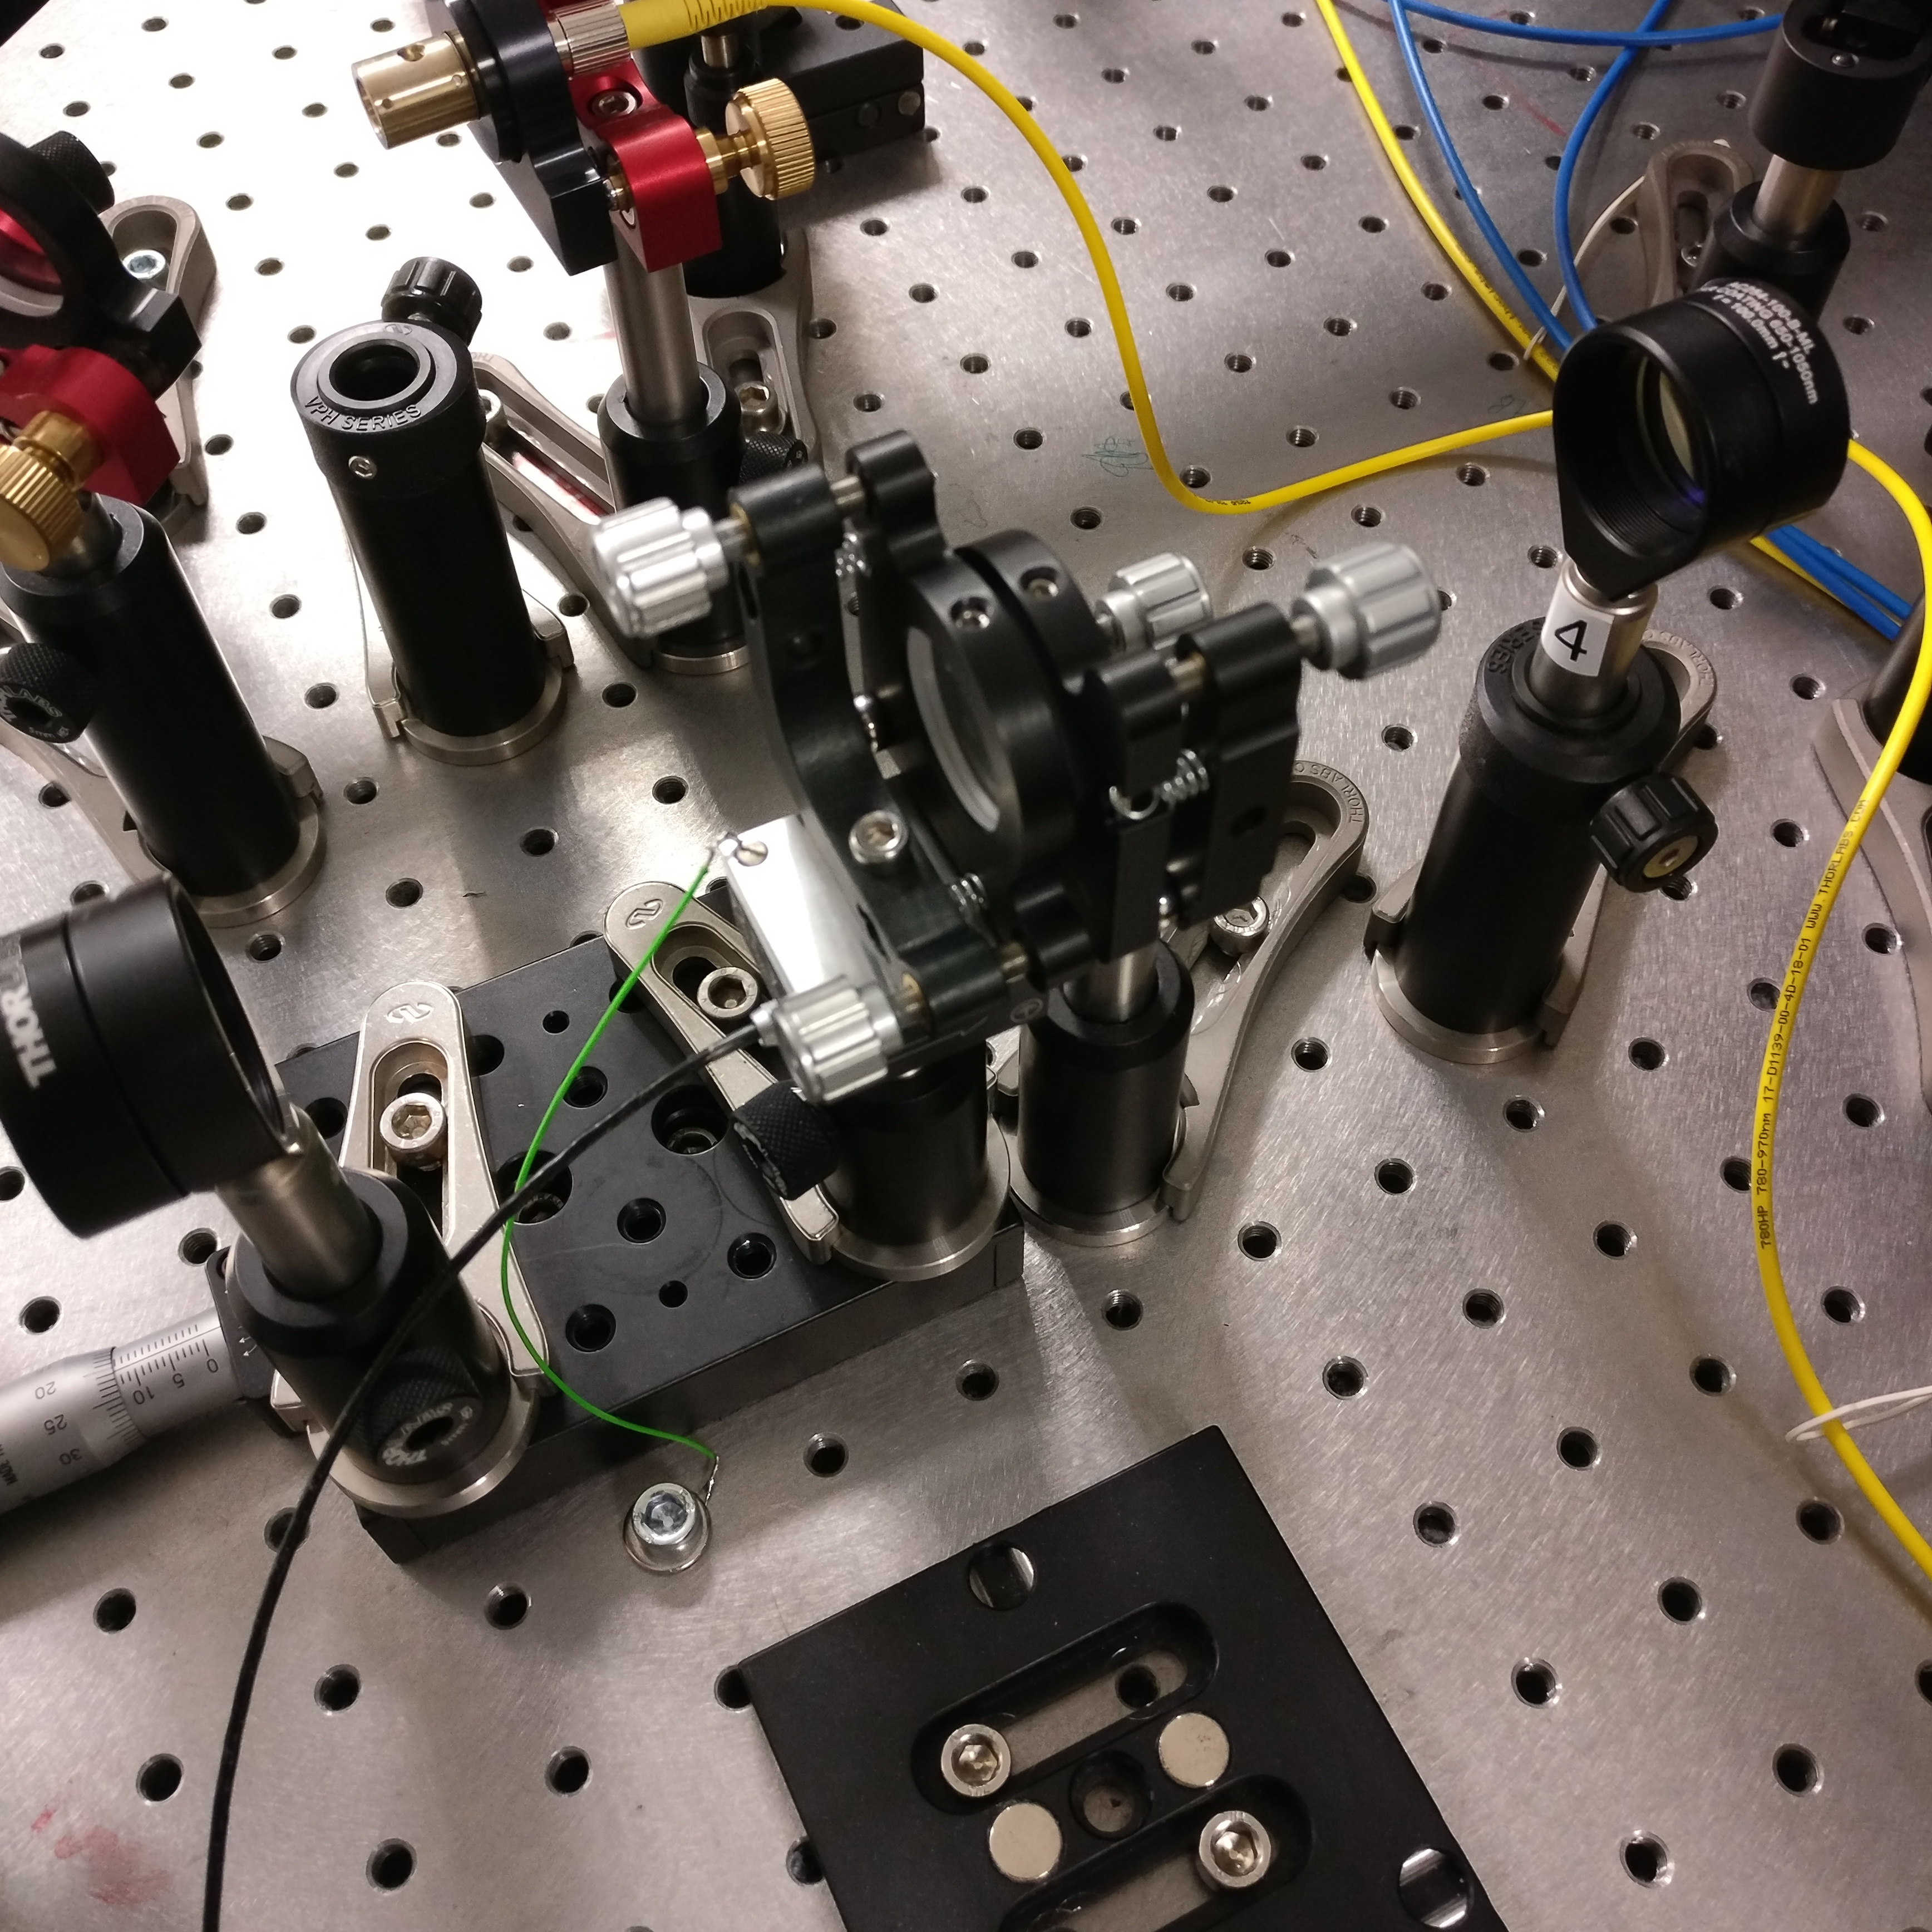
\includegraphics[width=0.95\textwidth]{figures/fabry-perot/setup/old}
		\caption{}
		\label{fig:old}
	\end{subfigure}%
	~ % An dieser Stelle kann ein zusätzlicher Zwischenraum eingebunden werden: ~, \quad, \qquad, \hfill usw.
	% Eine leere Zeile erzwingt, dass die zweite Grafik darunter erscheint.
	\begin{subfigure}[b]{0.48\textwidth}
		\centering
		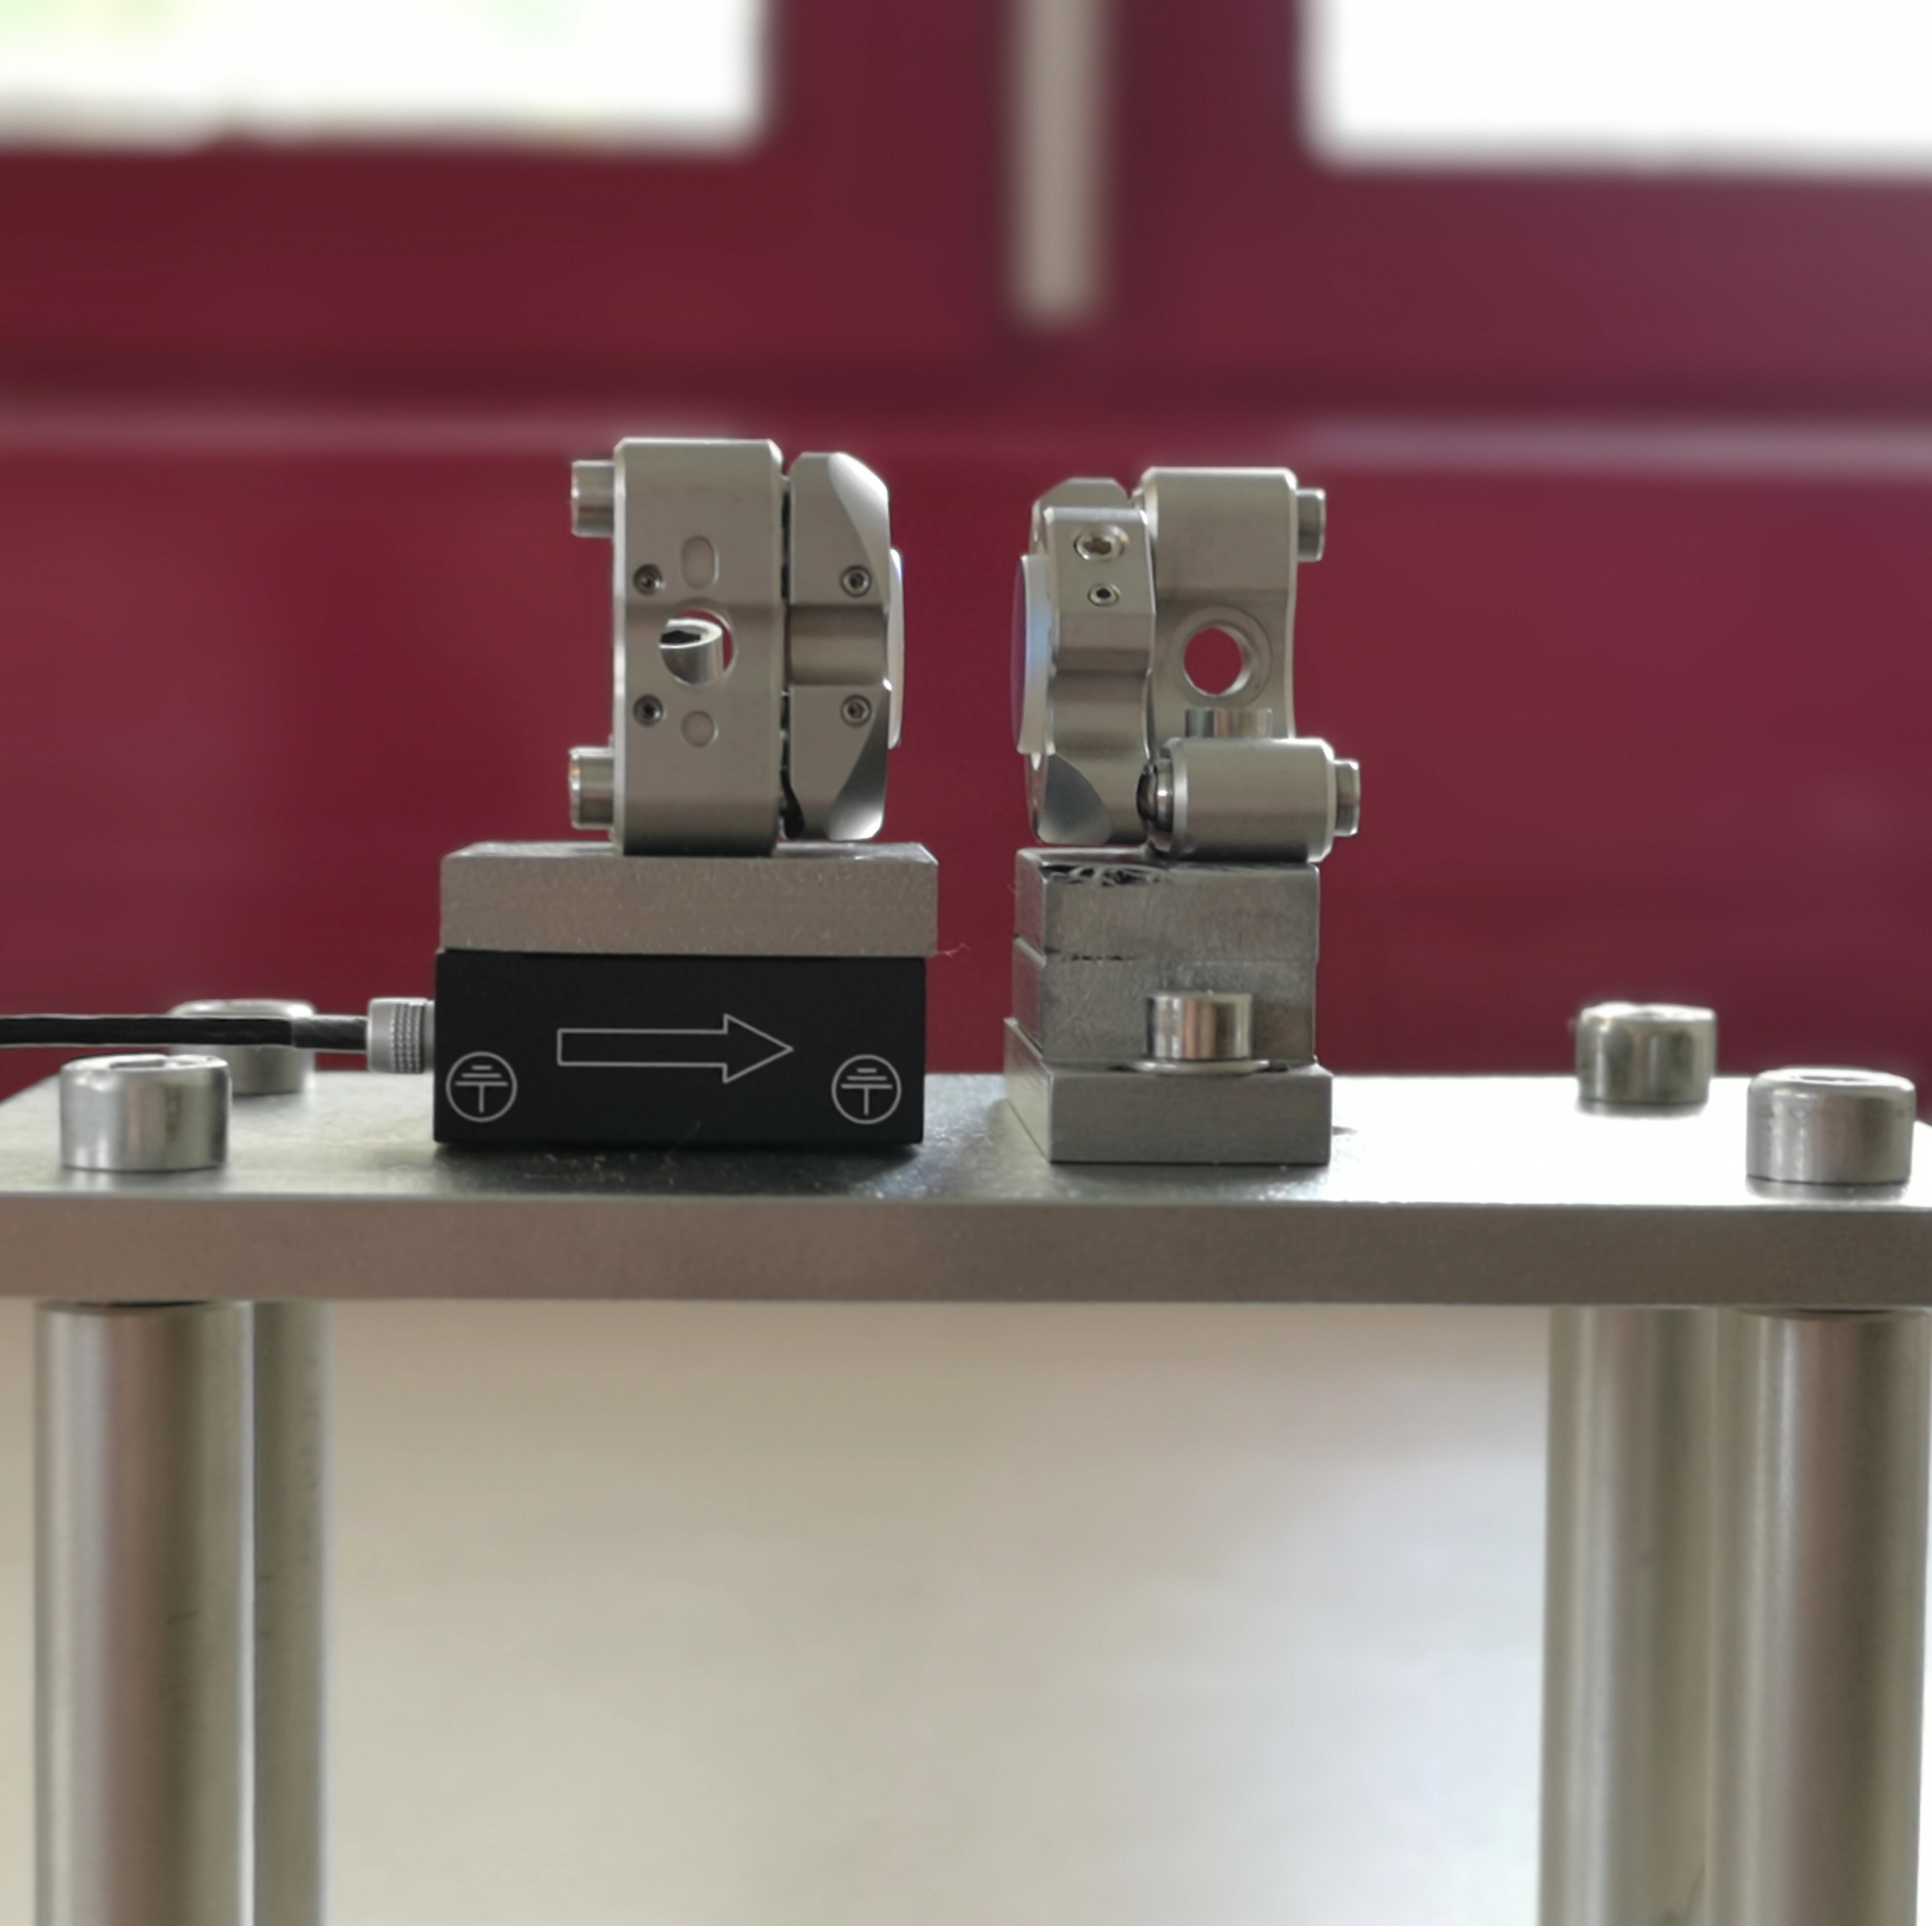
\includegraphics[width=0.95\textwidth]{figures/fabry-perot/setup/new}
		\caption{}
		\label{fig:new}
	\end{subfigure}
	\caption{}
	\label{fig:old-new-fpi}
\end{figure}

\begin{figure}[H]
	\centering
	\begin{subfigure}[b]{0.48\textwidth}
		\centering
		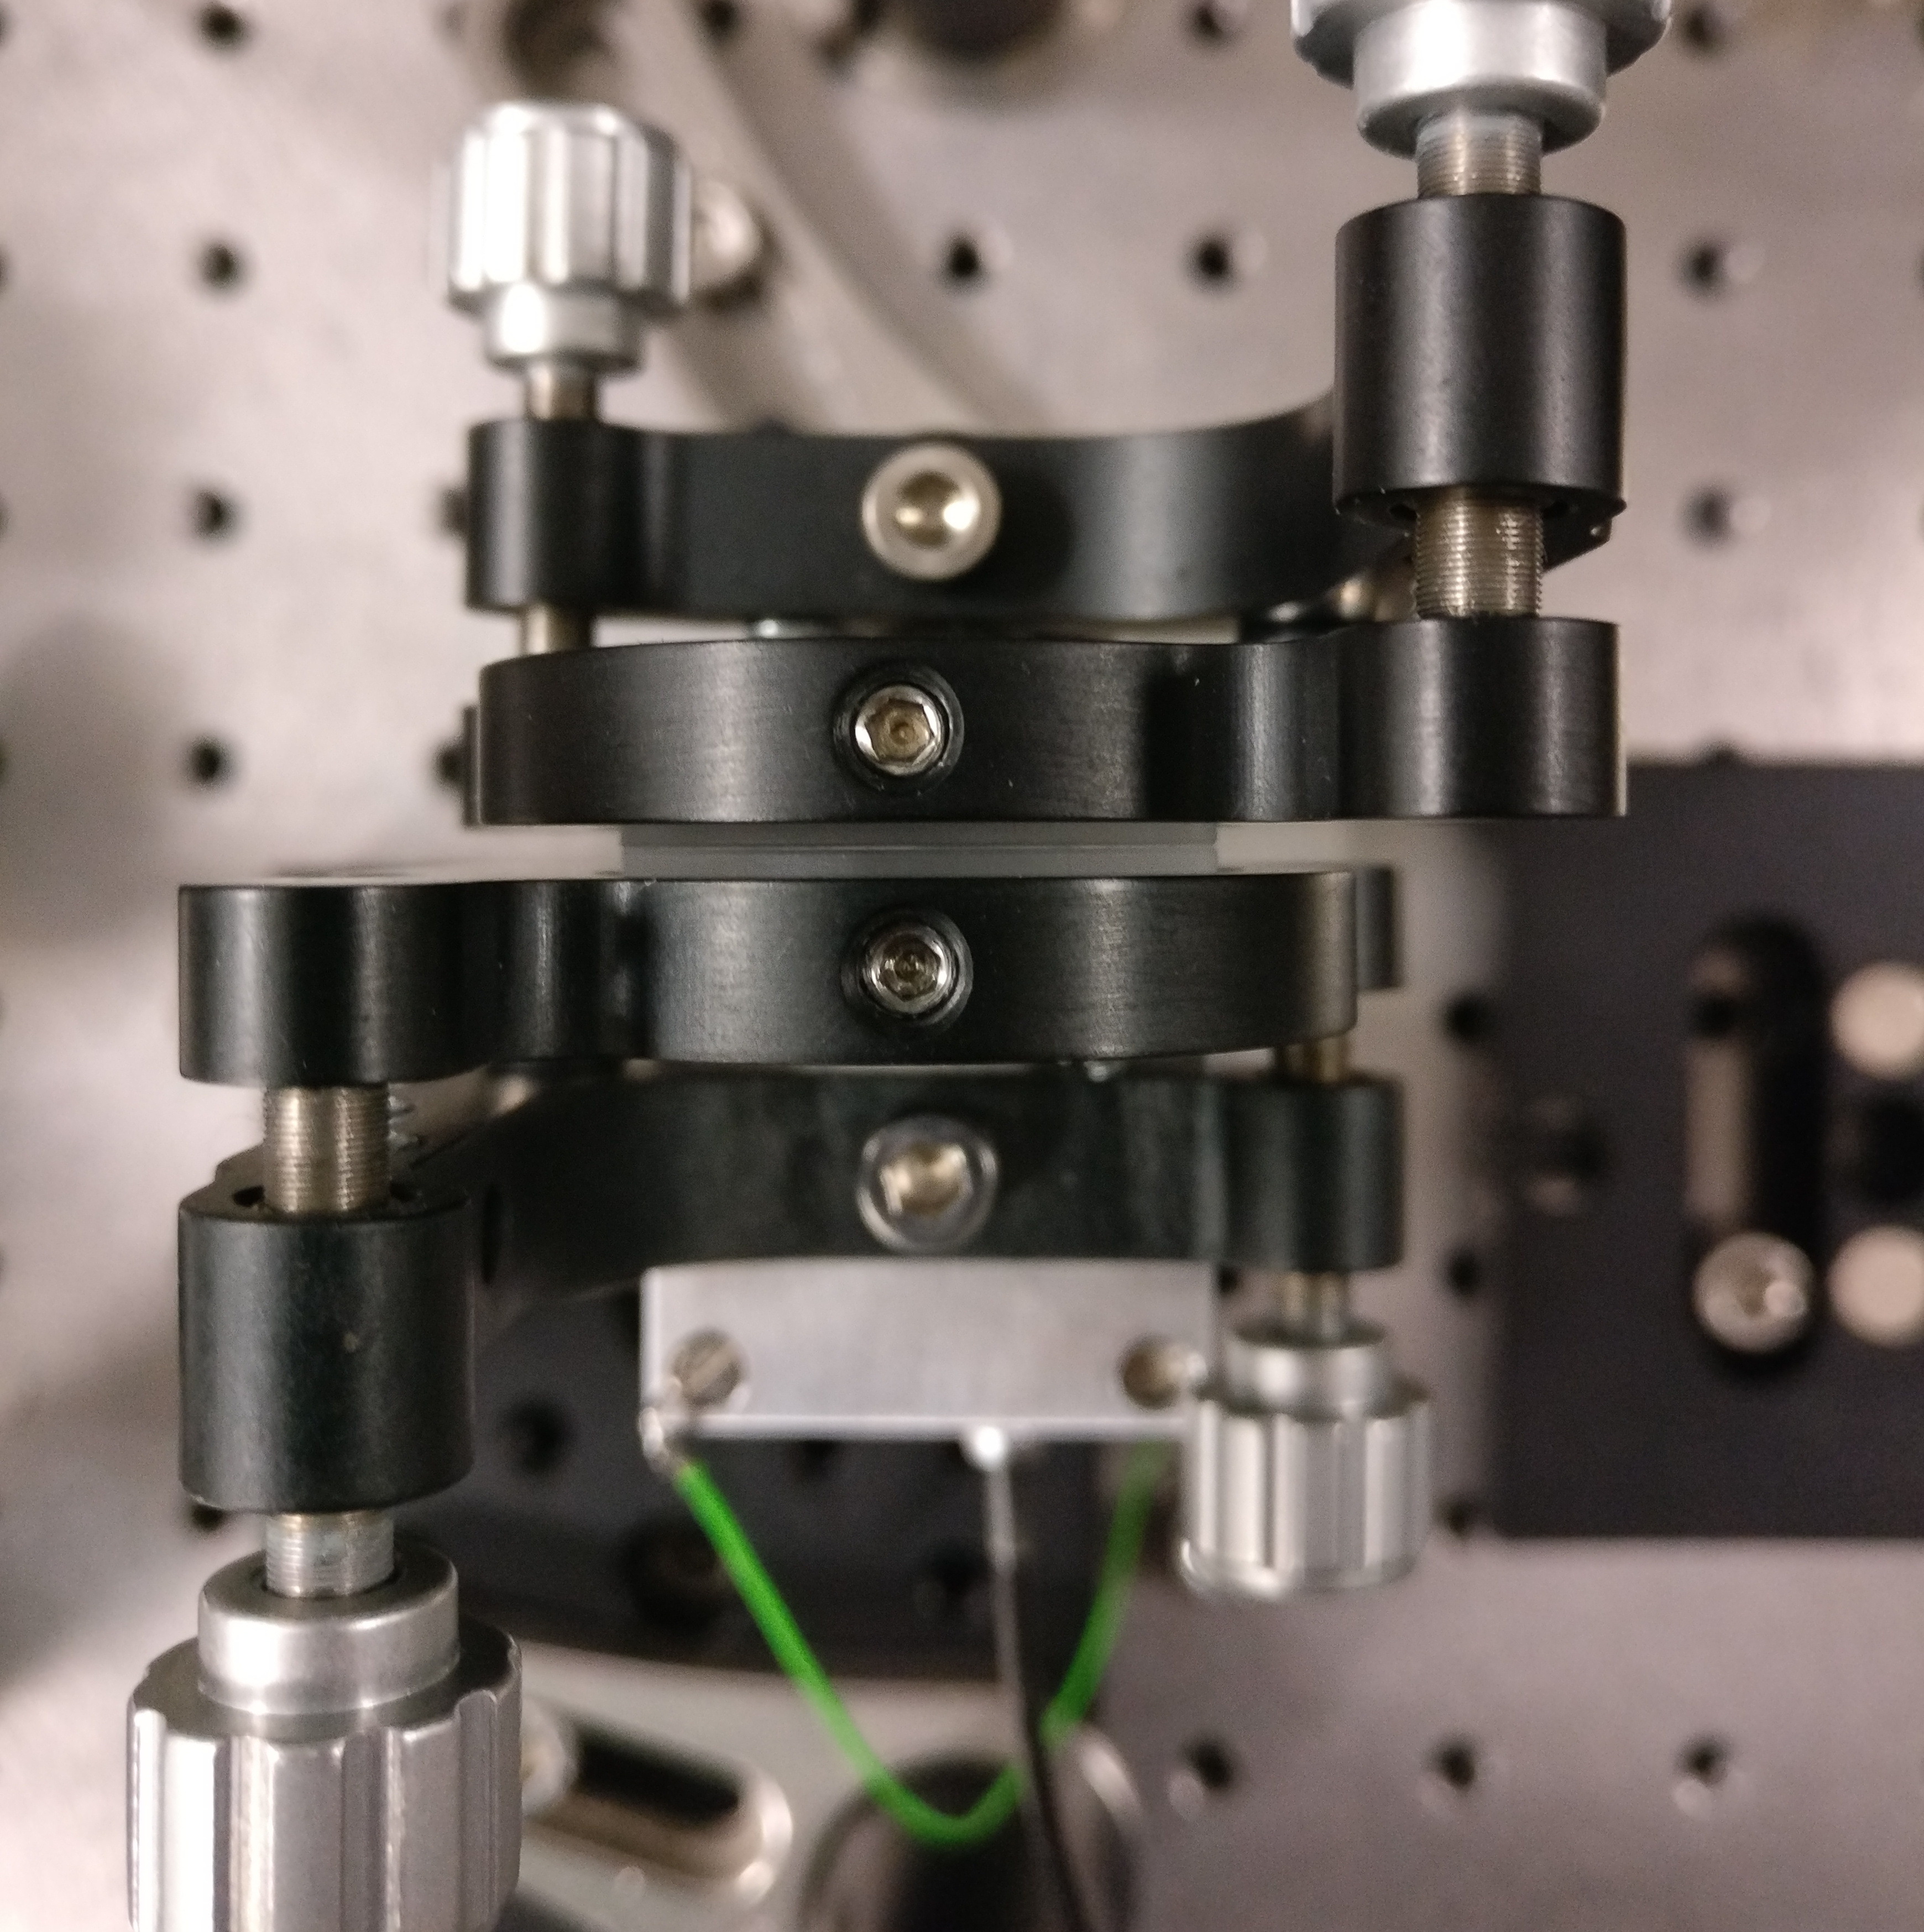
\includegraphics[width=0.95\textwidth]{figures/fabry-perot/setup/topview}
		\caption{}
		\label{fig:topview}
	\end{subfigure}%
	~ % An dieser Stelle kann ein zusätzlicher Zwischenraum eingebunden werden: ~, \quad, \qquad, \hfill usw.
	% Eine leere Zeile erzwingt, dass die zweite Grafik darunter erscheint.
	\begin{subfigure}[b]{0.48\textwidth}
		\centering
		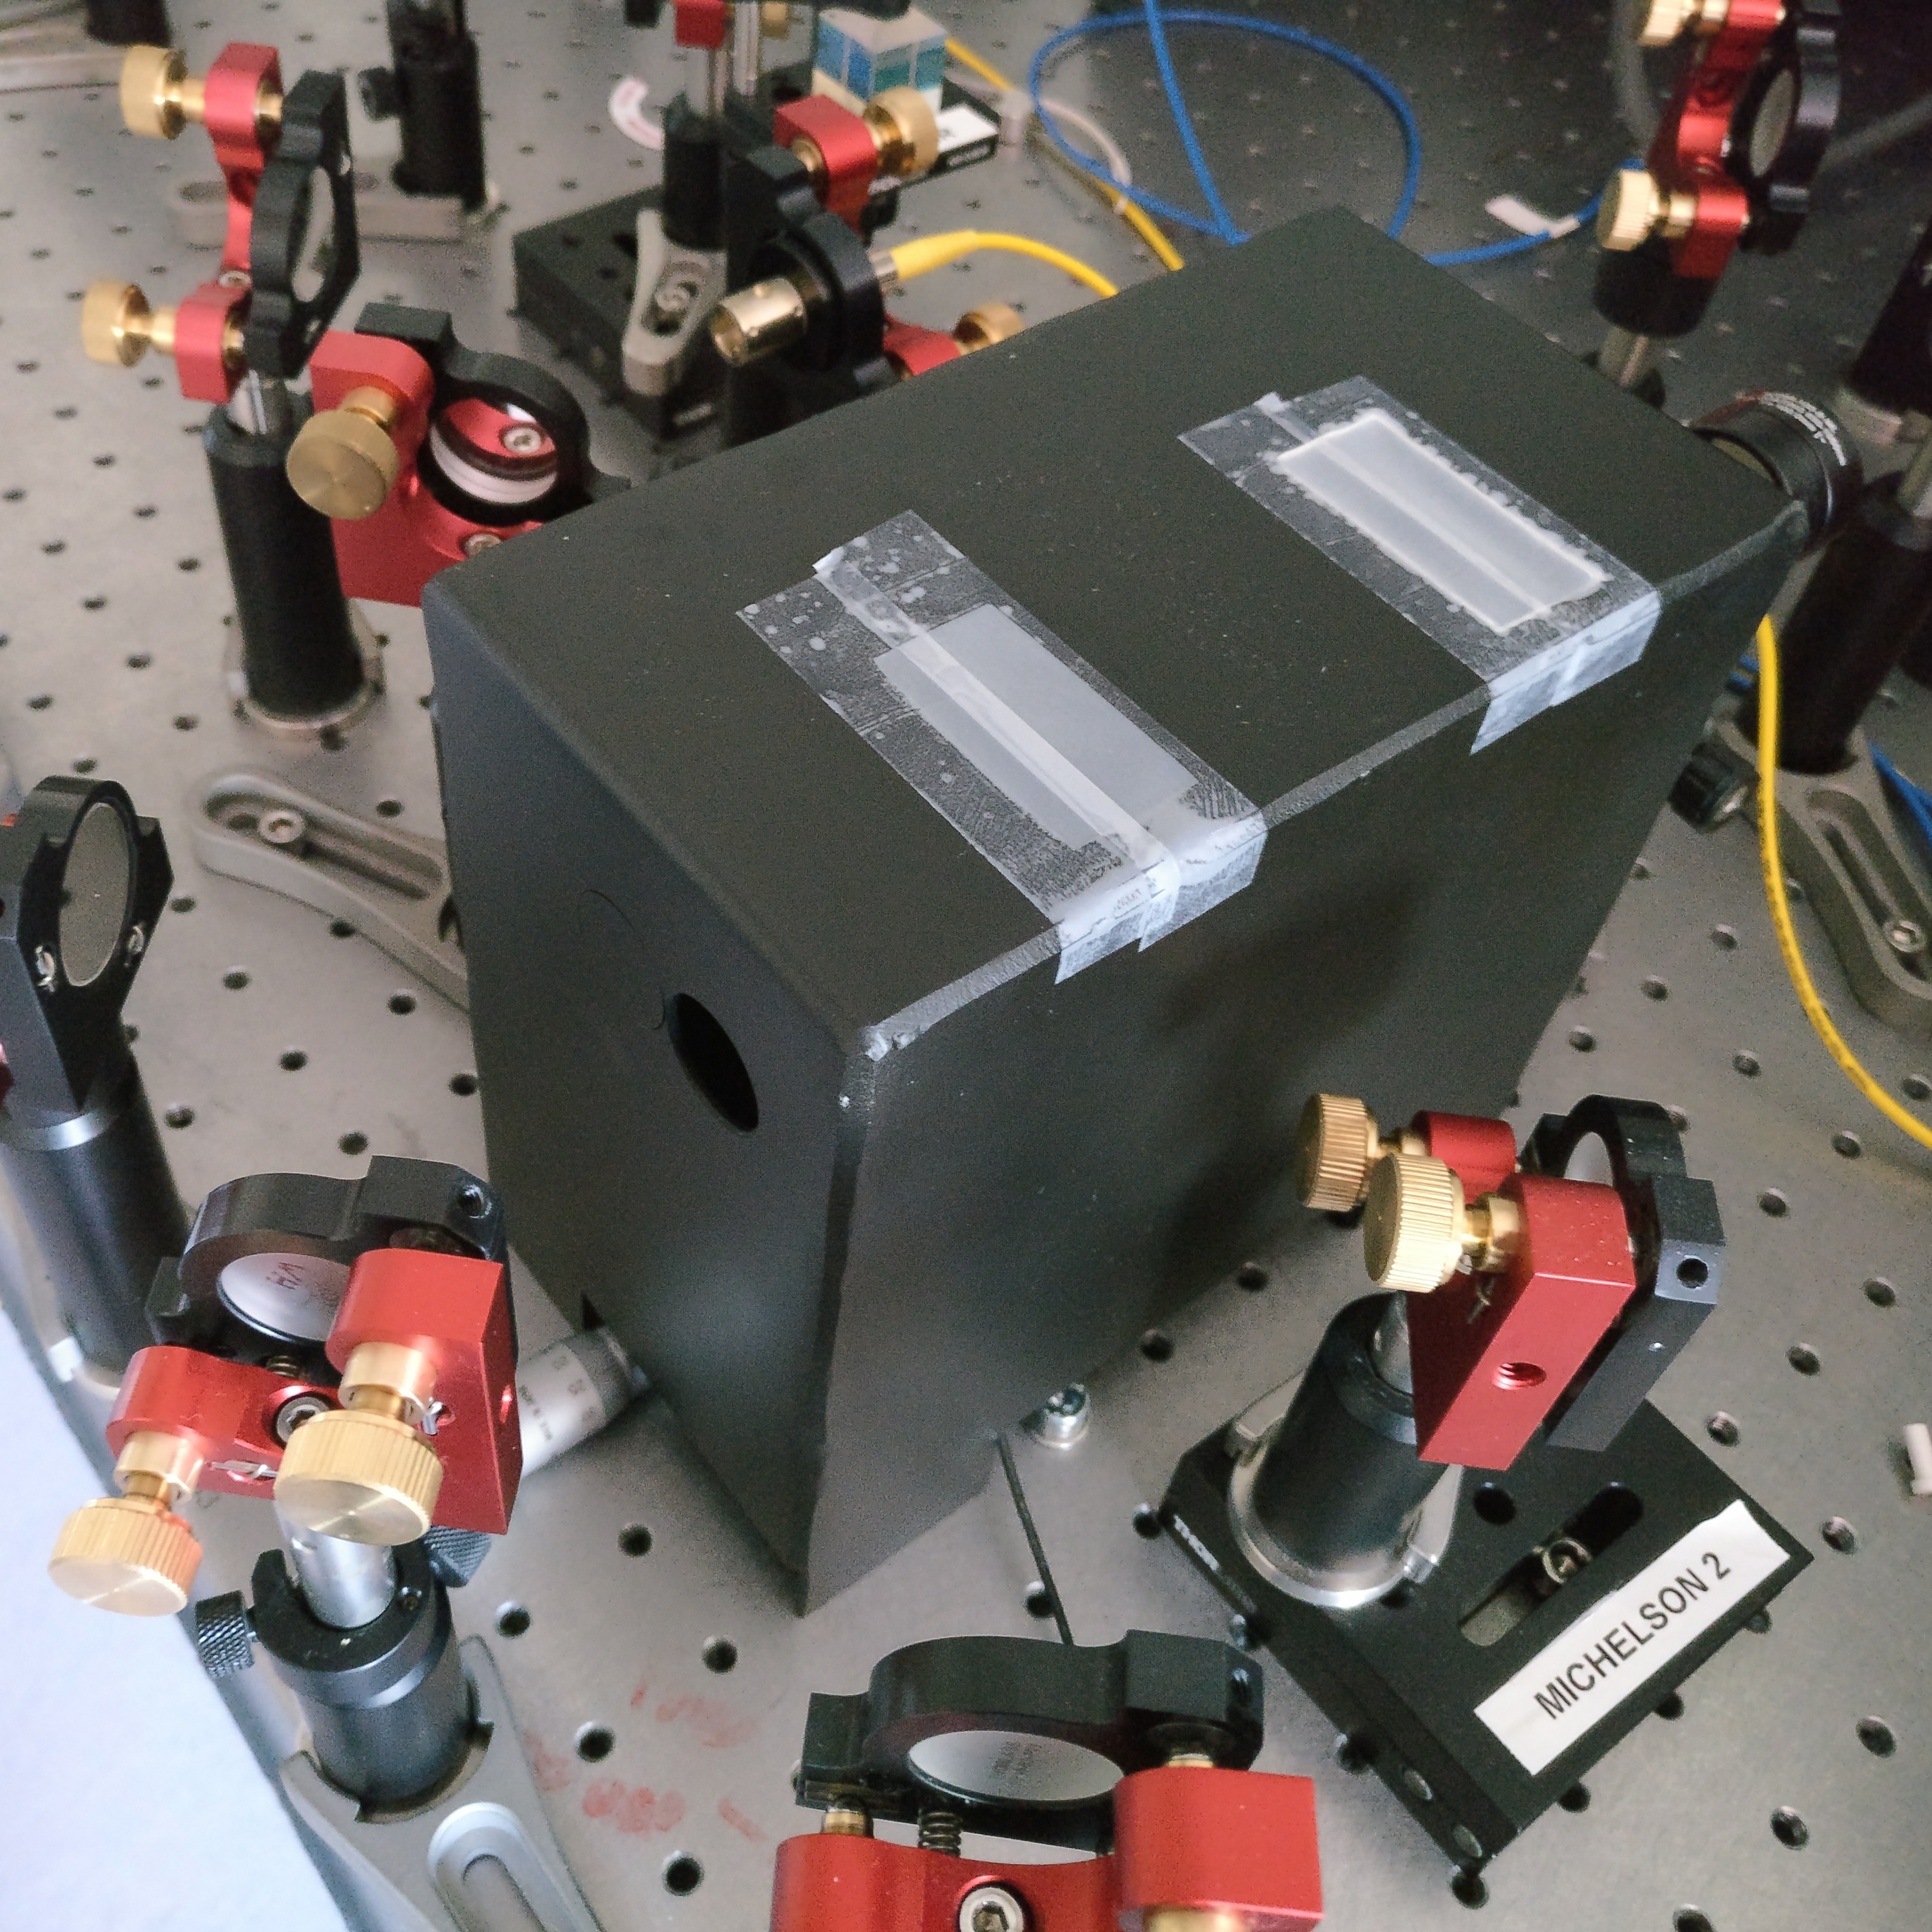
\includegraphics[width=0.95\textwidth]{figures/fabry-perot/setup/casing}
		\caption{}
		\label{fig:casing}
	\end{subfigure}
	\caption{}
	\label{fig:topview-casing}
\end{figure}


\subsection{Scanning mode with fast photodiodes}

\begin{figure}[H]
	\centering
	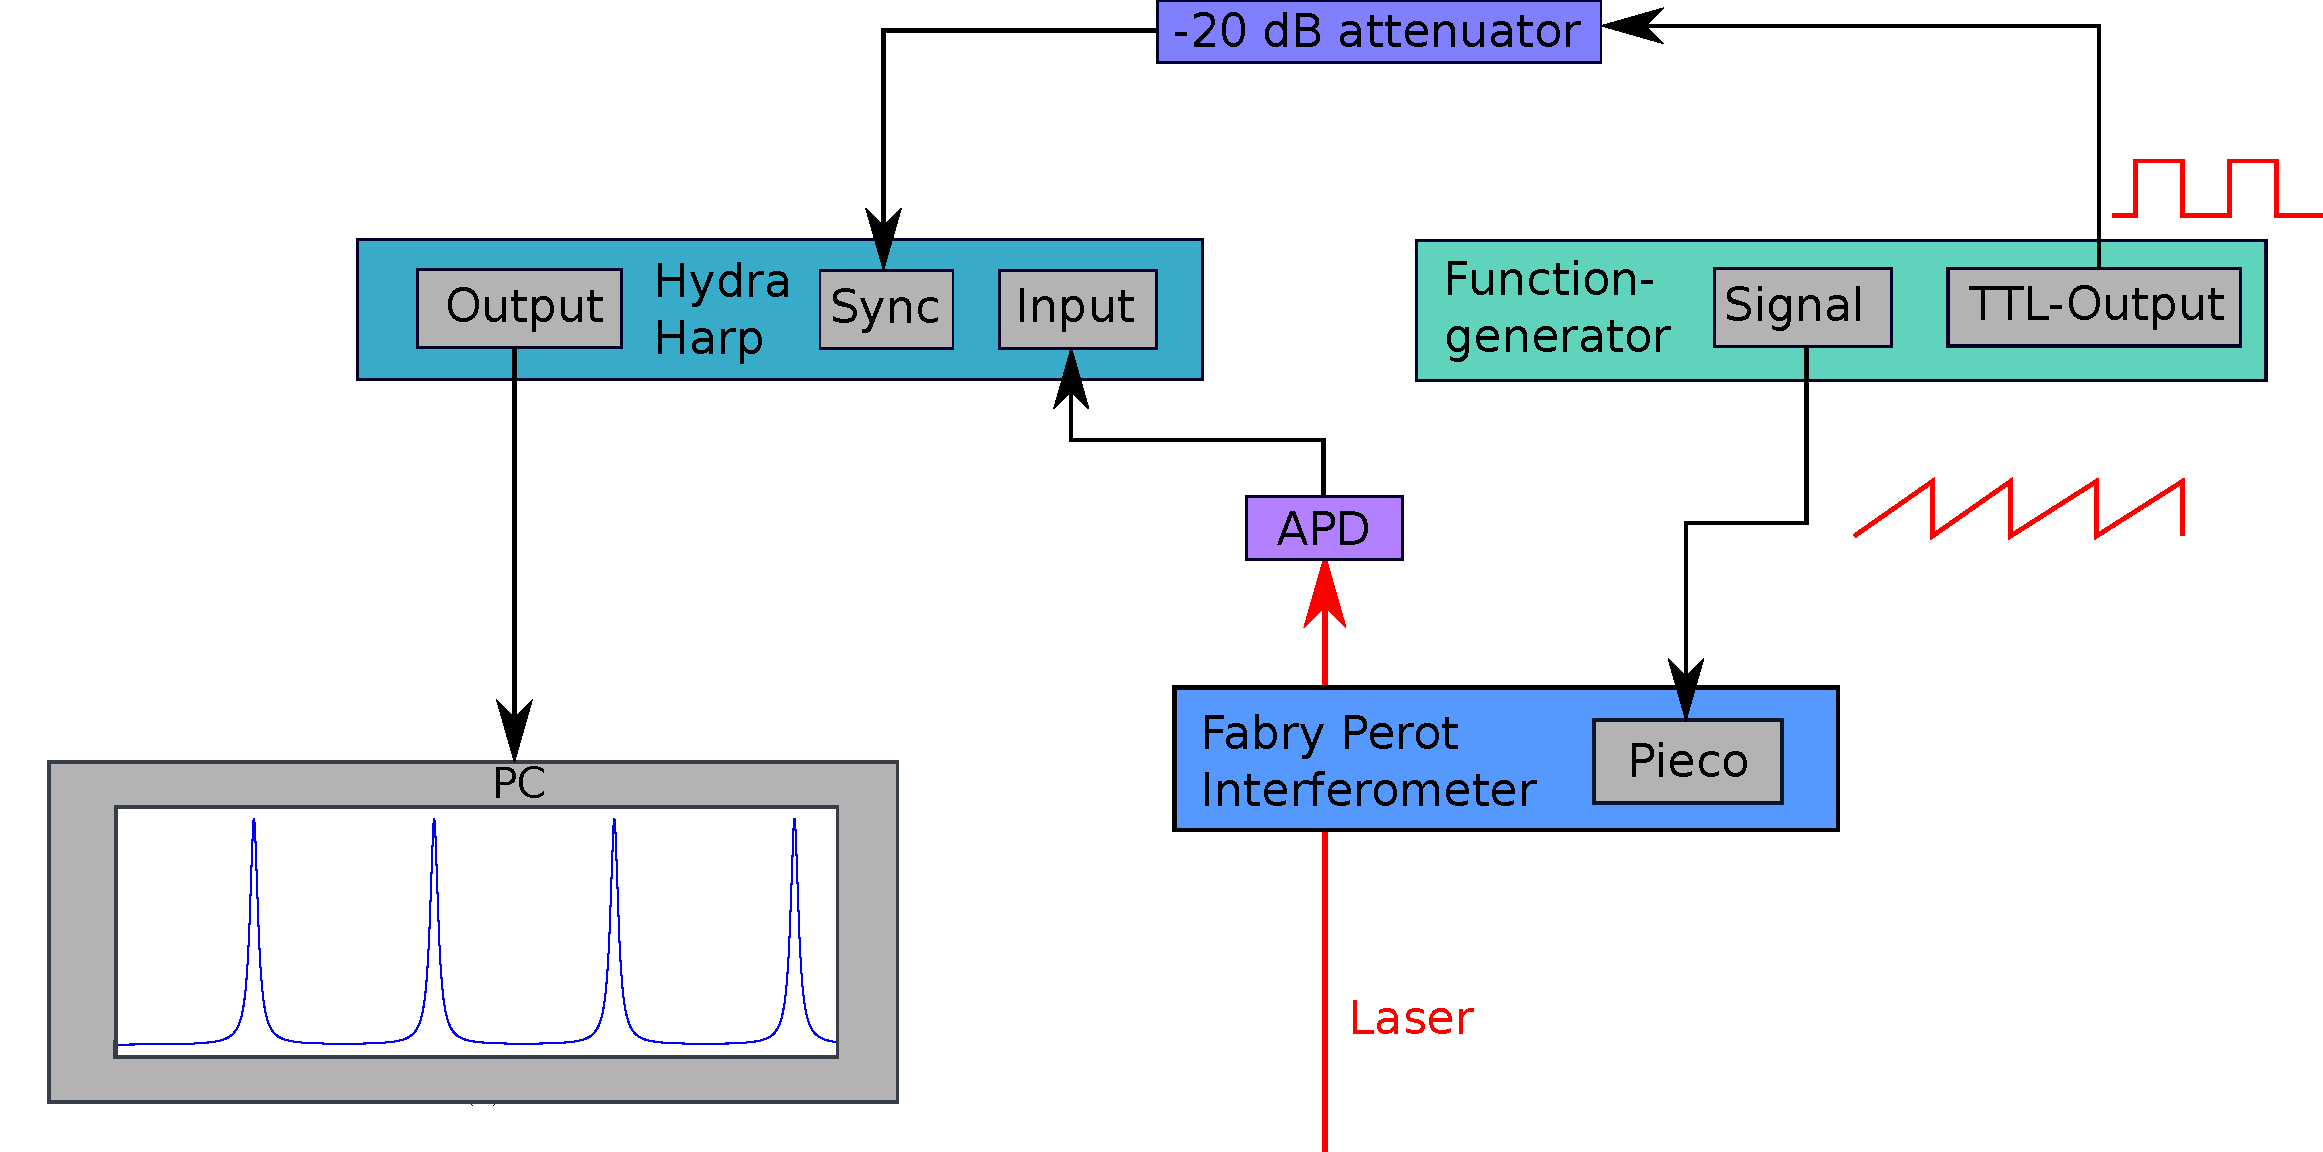
\includegraphics[width=\linewidth]{figures/fabry-perot/live-apd-setup}
	\caption{Live avalanche photodiode setup with using a function generator driving the piezo actuator of the FPI and the sync input of the correlation hardware.
	APDs are used because of their speed, allowing to live-adjusting the FPI-parameters.}
	\label{fig:live-apd-setup}
\end{figure}

Before the scanning \ac{FPI} can be used to measure \ac{QD} emission, it has to be aligned first.
\acp{APD} are used for aligning the \ac{FPI} as they are fast enough to measure the multiple free spectral ranges with a scanning frequency in the order of \si{\hertz}.
A function generator is used to drive the piezoelectrical actuator and the correlation hardware (here: Picoquant Hydraharp 400) correlates the measurements of the \ac{APD} with the TTL-output of the function generator.
The correlation hardware uses \ac{NIM} as input, while the TTL-output uses \ac{BNC}.
Because of that a \ac{NIM}-\ac{BNC} converter had to be used in between.
The complete setup is sketched in figure~\ref{fig:live-apd-setup}.

Figure~\ref{fig:2019-03-1914-10fabry-perot-live-apdrealigned} shows the measurement of the scanning \ac{FPI} with the \acp{APD}.
The scanning frequency is \SI{5}{\hertz} and the range is \SI{1}{\micro \meter}.
The measured finesse is $\approx 5$ and the free spectral range corresponds to \SI{280}{\nano \meter}.
The stability for one snapshot as visible here appears good, however the modes shift visibly over a longer period of time.


\begin{figure}[H]
	\centering
	\includegraphics[width=\linewidth]{figures/fabry-perot/plots/2019-03-19_14-10_Fabry-Perot-Live-APD_realigned}
	\caption{Measurement of scanning FPI with APDs.
	         The scanning frequency is \SI{5}{\hertz} and the range is \SI{1}{\micro \meter}.
             The measured finesse is $\approx 5$ and the free spectral range corresponds to \SI{280}{\nano \meter}.}
	\label{fig:2019-03-1914-10fabry-perot-live-apdrealigned}
\end{figure}
  
\subsection{Scanning mode with CCD}

\begin{figure}[H]
	\centering
	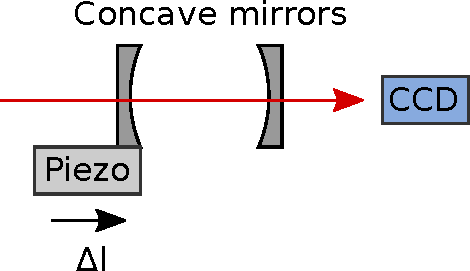
\includegraphics[width=0.5\linewidth]{figures/fabry-perot/setup/setup}
	\caption{Scanning Fabry Pérot interferometer with CCD}
	\label{fig:setup}
\end{figure}

In order to obtain the spectral emission of the input signal, the \ac{FPI} is used in the scanning mode.
Here one of the mirrors is attached to a piezoelectric actuator which moves the mirror stepwise after every measurement as shown in figure~\ref{fig:setup}. A minimal sketch of the setup is visible in figure~\ref{fig:setupflat}.





\section{Measurements and discussion}
\label{sec:fabry-measurements}

In the following measurements the \ac{FPI} was set up in the non-confocal mode and HeNe laser signals were used in order to align it.
This involves for one setting the mirrors coming before the \ac{FPI} so that the laser beam goes straight and centred through the \ac{FPI} mirrors and then setting the \ac{FPI} mirrors so that they are parallel and a single laser beam emerges as is shown in figure~\ref{fig:align-fpi}.


\begin{figure}[H]
	\centering
	\begin{subfigure}[b]{0.48\textwidth}
		\centering
		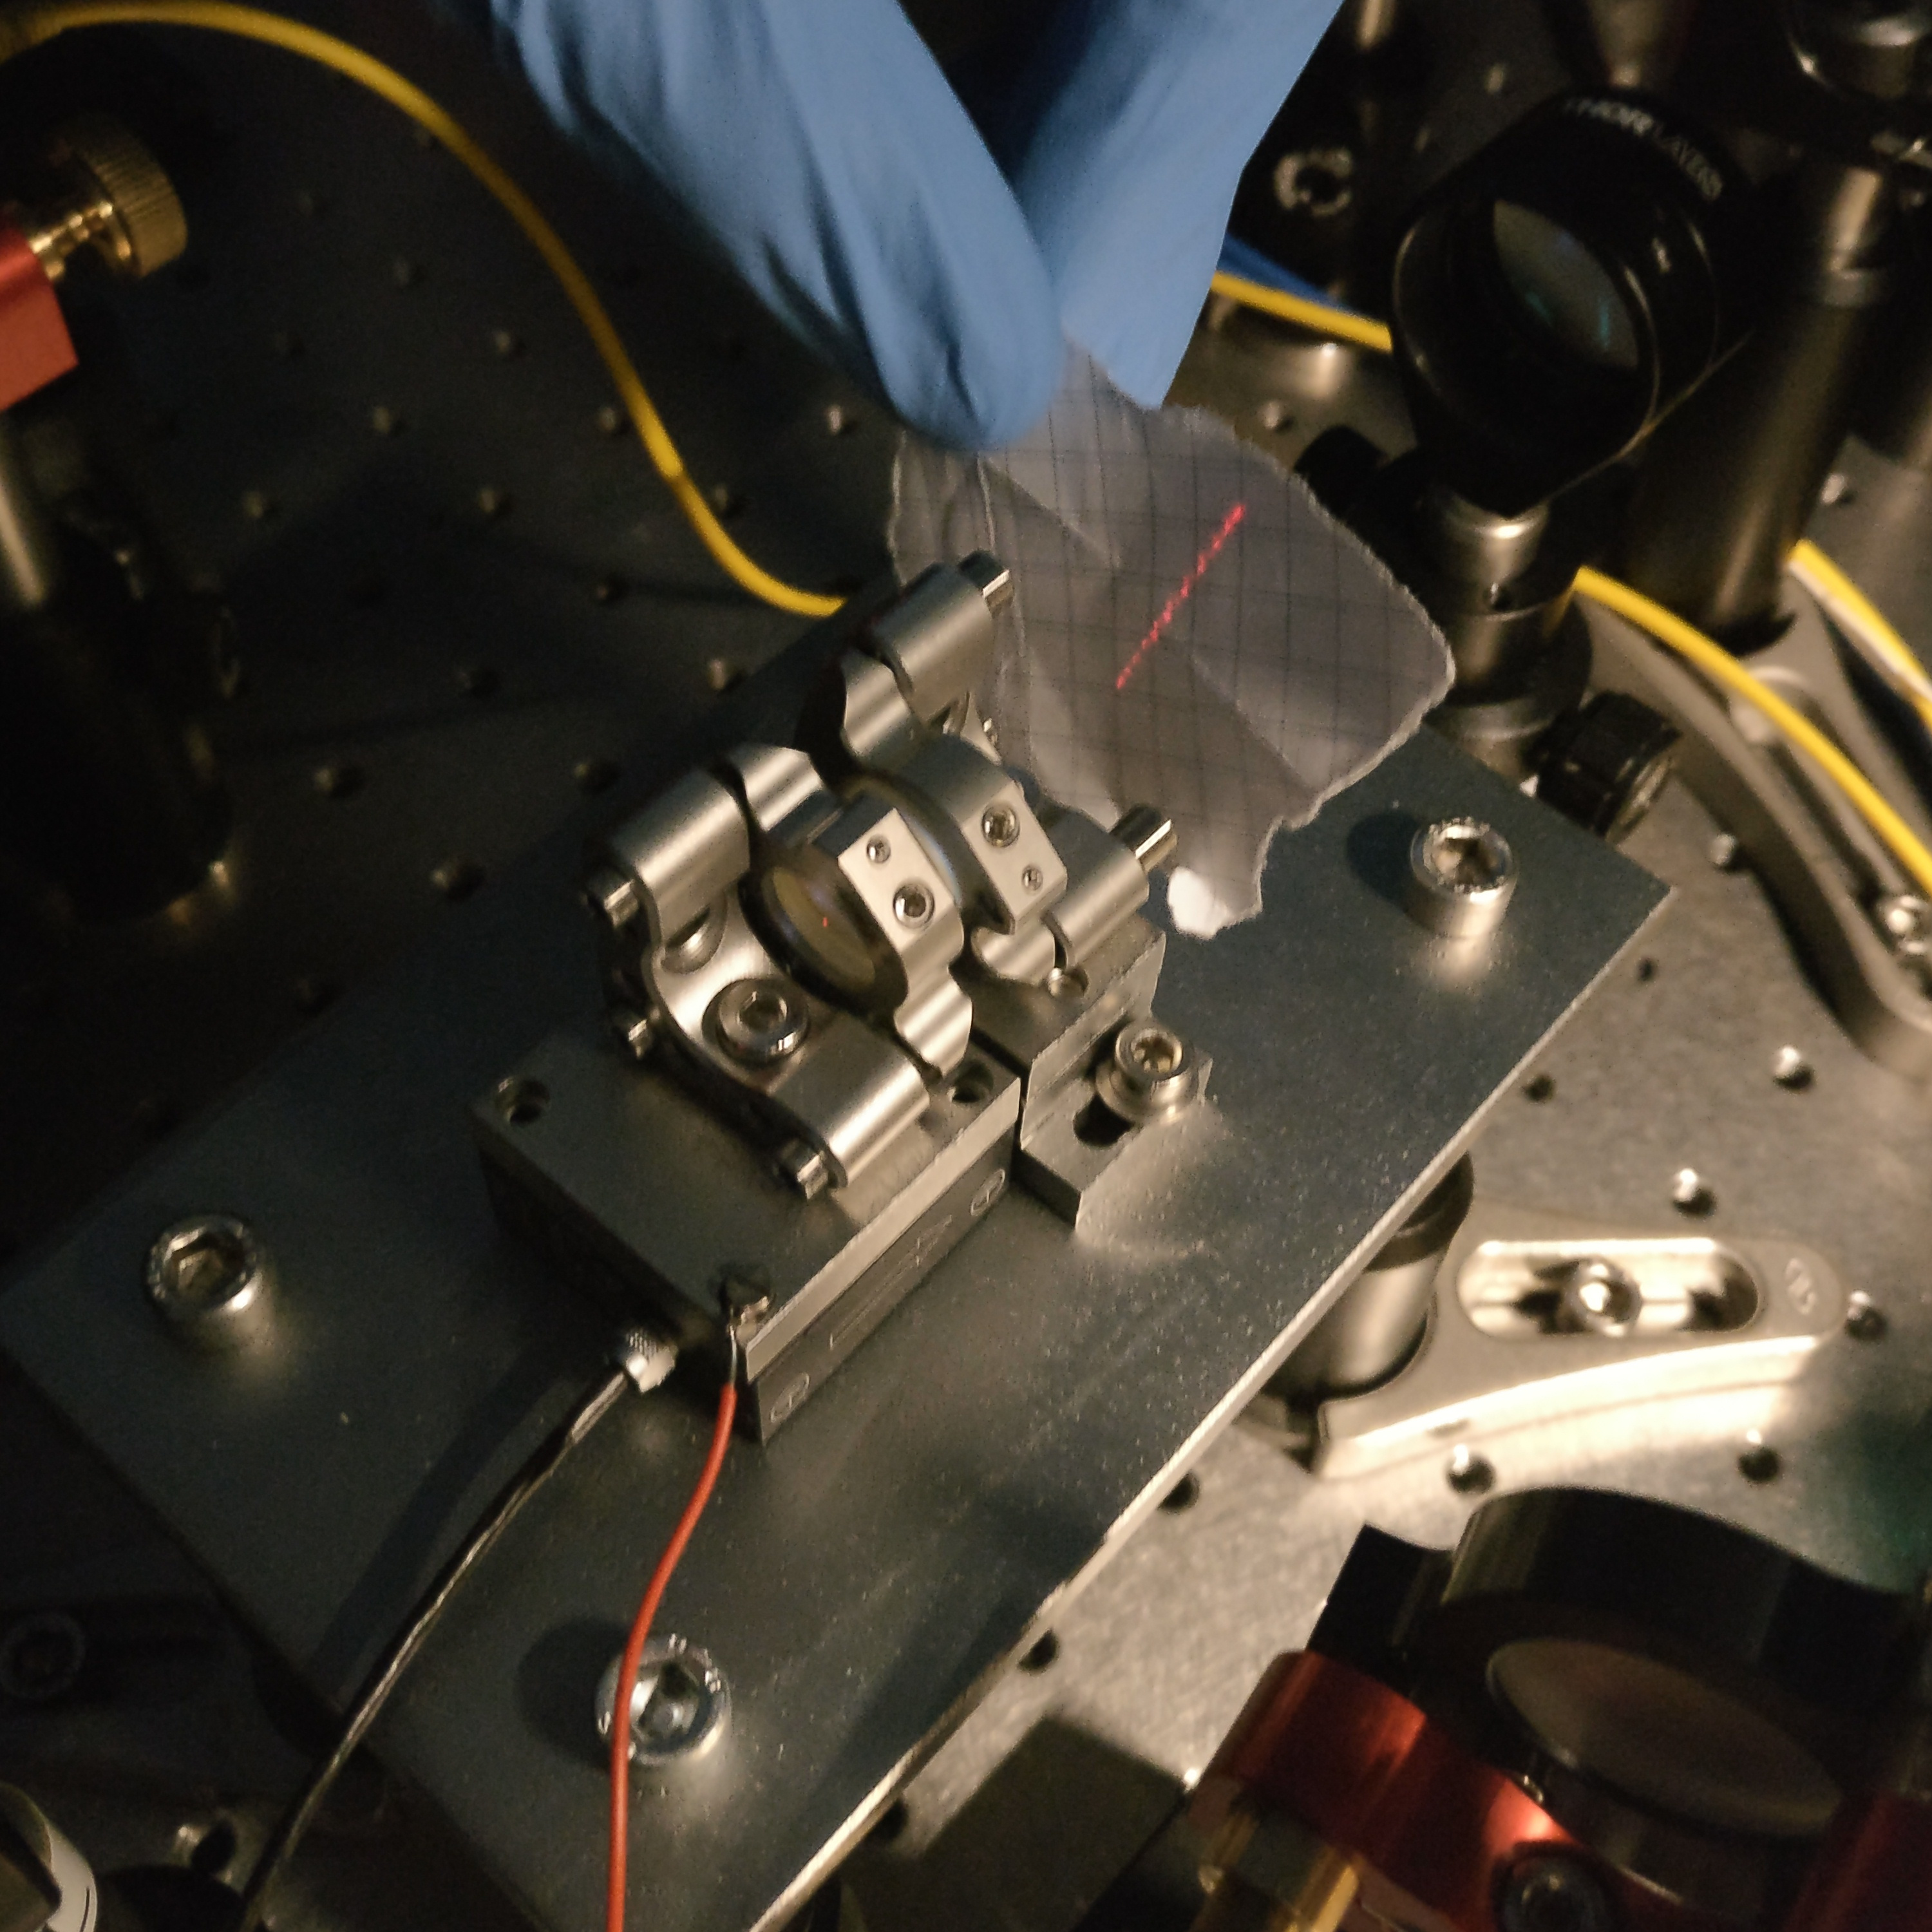
\includegraphics[width=0.95\textwidth]{figures/fabry-perot/setup/confocal-setup-higher-modes-1}
		\caption{}
		\label{fig:confocal-setup-higher-modes-1}
	\end{subfigure}%
	~ % An dieser Stelle kann ein zusätzlicher Zwischenraum eingebunden werden: ~, \quad, \qquad, \hfill usw.
	% Eine leere Zeile erzwingt, dass die zweite Grafik darunter erscheint.
	\begin{subfigure}[b]{0.48\textwidth}
		\centering
		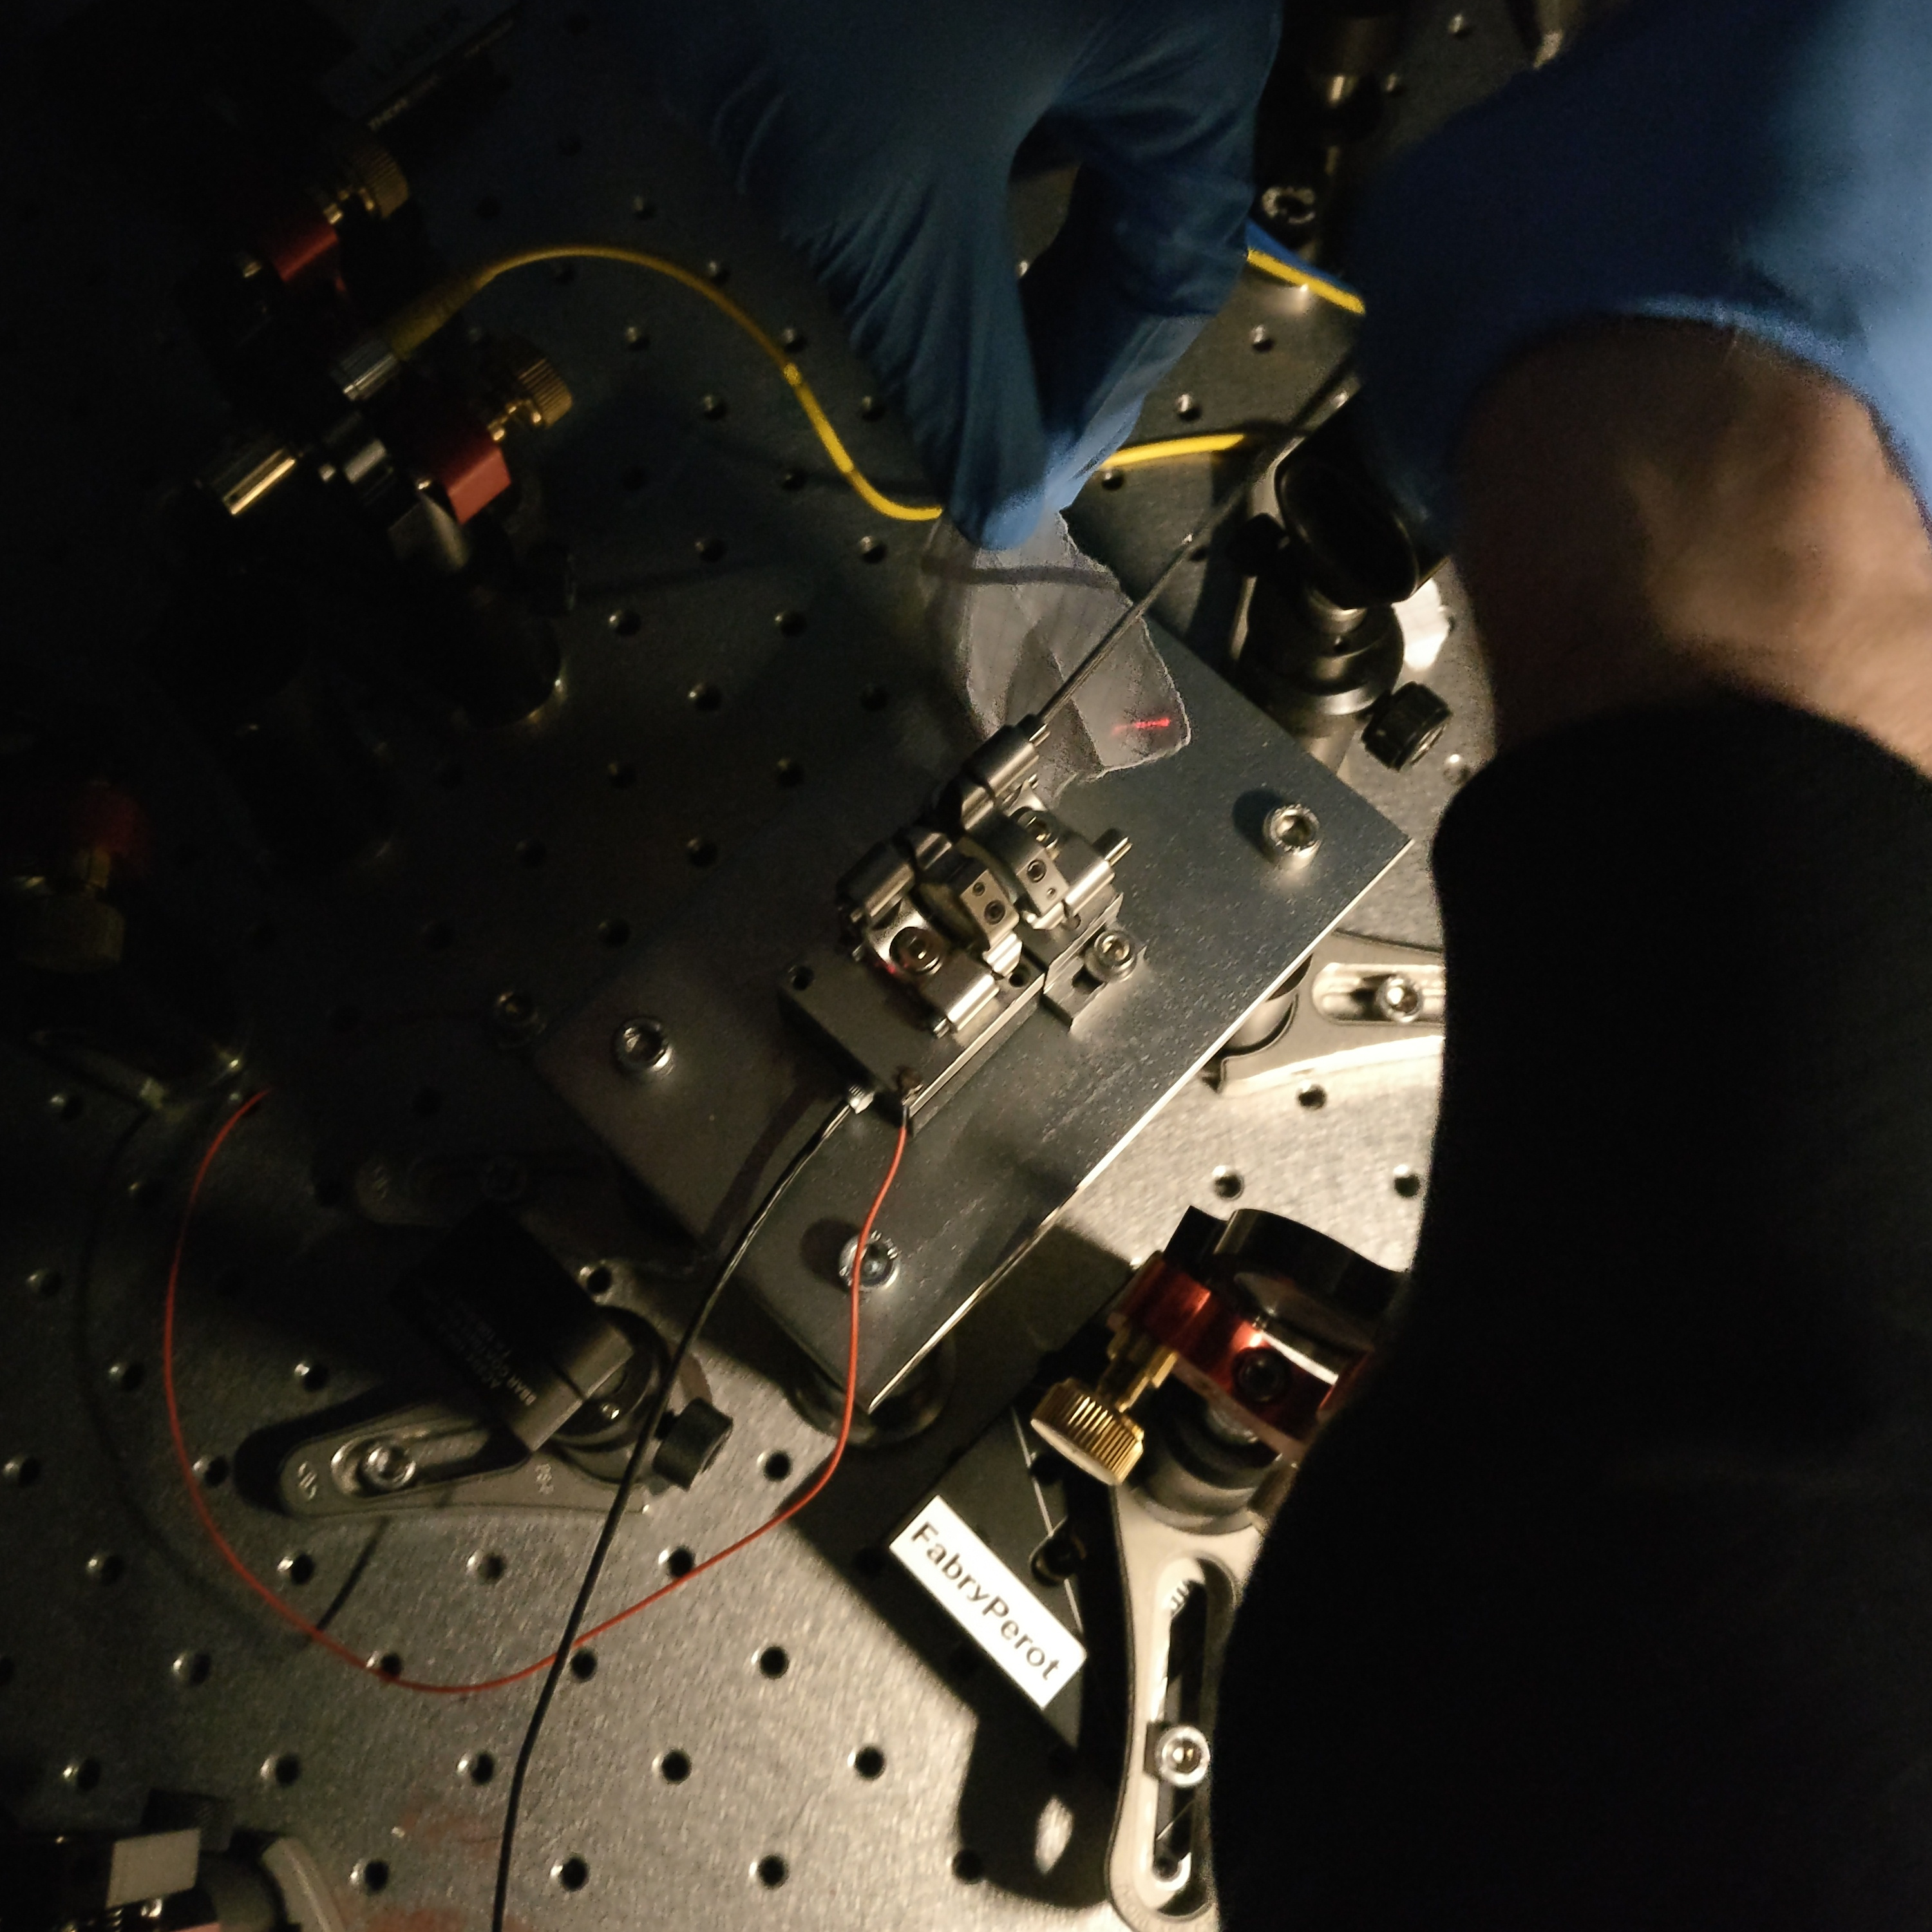
\includegraphics[width=0.95\textwidth]{figures/fabry-perot/setup/confocal-setup-higher-modes-2}
		\caption{}
		\label{fig:confocal-setup-higher-modes-2}
	\end{subfigure}
	\caption{Aligning the Fabry Pérot interferometer}
	\label{fig:align-fpi}
\end{figure}

Without spatial restriction strong TEM-modes of higher order are visible in figure~\ref{fig:measurement-fabry-perot-hene}(a).
To counteract, a pinhole is inserted and adjusted which results in the measurement visible in figure~\ref{fig:measurement-fabry-perot-hene}(b).

\begin{figure}[H]
	\centering
	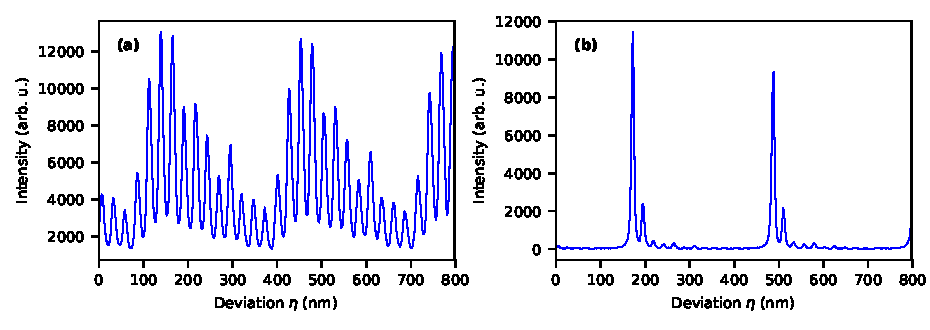
\includegraphics[width=\linewidth]{figures/fabry-perot/plots/measurement-fabry-perot-HeNe}
	\caption{Transmission measurement of FPI with ground mirror distance $l \approx \SI{2}{\milli \meter}$ and HeNe laser. (a) was aligned without spatial filtering with a pinhole and (b) involved a pinhole.}
	\label{fig:measurement-fabry-perot-hene}
\end{figure}

Set up like this, the GaAs \ac{QD} sample AS208 was measured.
First a polarization map of the exciton was recorded in order to determine the \ac{FSS} $E_{FSS}=\SI{24.42 (39)}{\micro \electronvolt}$ with the data shown in figure~\ref{fig:measurement-fabry-perot-dot-exciton-pol-map}.
\todo{how does this work. Explain more details, this is not trivial}

\begin{figure}[H]
	\centering
	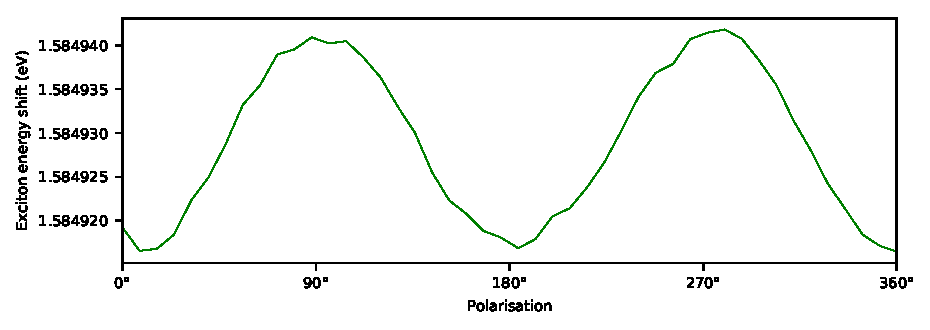
\includegraphics[width=\linewidth]{figures/fabry-perot/plots/measurement-fabry-perot-dot-exciton-pol-map}
	\caption{Polarization map of exciton of QD in sample AS208.}
	\label{fig:measurement-fabry-perot-dot-exciton-pol-map}
\end{figure}

Afterwards the output of the \ac{QD} through the \ac{FPI} was measured while the mirror distance was stepwisely changed which is shown in figure~\ref{fig:measurement-fabry-perot-dot-biexciton-fss}.
The x-scale on the top of figure~\ref{fig:measurement-fabry-perot-dot-biexciton-fss} was calculated by correlating the distance between the two adjacent peaks with the \ac{FSS} determined with the data of figure~\ref{fig:measurement-fabry-perot-dot-exciton-pol-map}.
For this \ac{QD} results in a conversion between the deviations $\eta=\SI{1}{\nano \meter} \equalhat \zeta = \SI{1.19 (2)}{\micro \electronvolt}$.
\todo{What does this comparison tell us? Did it fit the calculation? Where are the side peaks we saw in the HeNe measurement? What a about the stability? Are there calculations, expected temperature drifts, etc. Are there differences between the expected Finesse and the measured one, and why? Is this expected?}


\begin{figure}[H]
	\centering
	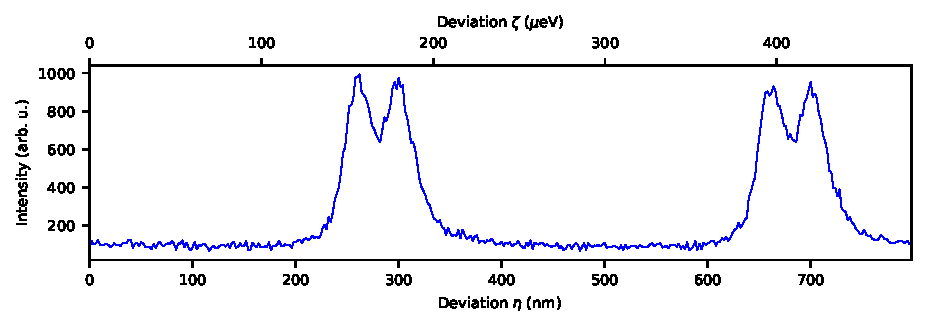
\includegraphics[width=1\linewidth]{figures/fabry-perot/plots/measurement-fabry-perot-dot-biexciton-FSS}
	\caption{Finestructure measurement of biexcition of QD in sample AS208 by passing thorugh FPI and sweeping the mirror distance.
	Ground mirror distance was  $l \approx \SI{2}{\milli \meter}$.}
	\label{fig:measurement-fabry-perot-dot-biexciton-fss}
\end{figure}





% !TEX root = ../masterthesis.tex
\chapter{Summary and outlook}
\label{cha:summary}
This thesis describes the efforts to improve excitation of quantum dots (\ac{QD}s) and to build up a scanning \acl{FPI} which allows to resolve fine details of \ac{QD} emission spectra.
In order to excite the \ac{QD} via adiabatic rapid passage the chirp of the exciting laser beam needs to be deterministically adjustable.
This again requires to build up a setup suitable to manipulate the chirp and a way to determine the chirp parameter $\alpha$.
The laser beam is measured with an interferometric auto correlator, however the shape of this measurement depends only weakly on $\alpha$.
Therefore the numerical filter \ac{MOSAIC} is applied, which resulted in a signal of which the lower envelope depends strongly on $\alpha$.
The simulations show that a fit of the lower envelope of the \ac{MOSAIC} signal allows to determine the chirp parameter.
A pulse expander is built up, with the goal of deterministically adjusting the chirp by adapting the distance between two optical elements.
Measurements with a Ti:Sa laser with and without a pulse expander are conducted, which suggested that the laser signal without the pulse expander is already heavily chirped.
That is why future experiments will investigate different laser models and then compare the measurements with the chirped signal after the pulse expander.
Additionally, the laser emission shape will be described more accurately in future simulations with a frequency comp instead of a simple Gaussian in order to better understand the influence of this approximation.
Afterwards, \acp{QD} will be excited via adiabatic rapid passage.

The second topic of this thesis is the build-up of a scanning \ac{FPI}.
Simulations show that common optical components are sufficient to build up a \ac{FPI} which is able to resolve the zero-phonon line of the \ac{QD} emission.
Measurements with planar mirrors show the instability of this arrangement, which is why we switch to planar-concave mirrors.
The \ac{FPI} is aligned with a HeNe laser and fast photodiodes, allowing to adjust the optical components of the \ac{FPI} with direct feedback.
Together with mode matching and spatial filtering, this allows to resolve the fine structure splitting of the excitonic energy levels of the \ac{QD}.
The transmission is determined to be \SI{5}{\percent} and the thermal shift of the \ac{FPI} modes is estimated to be $\approx \SI{66}{\percent}$ of one free spectral range per Kelvin.
Both the transmission and the thermal drift are sufficient for resolving the splitted excitonic emission line, however the measured finesse of $45$ is too low to resolve near-Fourier-limited zero-phonon-lines.
Also mode-matching and spatial-filtering is time consuming and error prone, which makes them impractical for common measurements.
Therefore, the \ac{FPI} is going to be used with mirrors of higher reflectivity and lower curvature radius and order to gain higher finesse and to use the \ac{FPI} in the confocal mode.
Here the curvature radius is equal to the mirror distance, which removes the flexibility to change resolution and free spectral range of the \ac{FPI}.
However, the cavity becomes mode-degenerated and therefore liberates from mode matching considerations.


\appendix                       %% closes main document, appendix follows until end; only available in book-classes
\addpart*{Appendix}             %% adding Appendix to tableofcontents

\chapter{Acronyms}
\begin{acronym}[TDMA]
	\acro{QKD}{quantum key distribution}
	\acro{QD}{quantum dot}
	\acro{FSS}{fine structure splitting}
	\acro{MBE}{molecular beam epitaxy}	
	\acro{CB}{conduction band}
	\acro{VB}{valence band}
	\acro{X}{exciton}
	\acro{XX}{biexciton}
	\acro{ZPL}{zero phonon line}
	\acro{PSB}{phonon side band}	
	\acro{HBT}{Hanbury-Brown-Twiss}
	\acro{BS}{beam splitter}
	\acro{ARP}{adiabatic rapid passage}
	\acro{IAC}{interferometric autocorrelation}
	\acro{MOSAIC}{modified-spectrum autointerferometric correlation}
	\acro{FPI}{Fabry Pérot interferometer}
	\acro{FWHM}{full width at half maximum}
	\acro{APD}{avalanche photodiode}
	\acro{CCD}{charge-coupled device}
\end{acronym}


\printbibliography              %% remove, if using BibTeX instead of biblatex
% \include{further_ressources}  %% this is a suggestion: you have to create this file on demand



%%%% end{document}
\end{document}
%% vim:foldmethod=expr
%% vim:fde=getline(v\:lnum)=~'^%%%%\ .\\+'?'>1'\:'='
%%% Local Variables:
%%% mode: latex
%%% mode: auto-fill
%%% mode: flyspell
%%% eval: (ispell-change-dictionary "en_US")
%%% TeX-master: "main"
%%% End:
